\documentclass[a4paper,12pt]{article}
\usepackage[margin=2cm]{geometry}

% Pacchetti utili di base
\usepackage[utf8]{inputenc}   % codifica dei caratteri
\usepackage[T1]{fontenc}      % font encoding
\usepackage[italian]{babel}   % lingua italiana
\usepackage{graphicx}         % immagini
\usepackage{hyperref}         % link cliccabili
\usepackage{amsmath}          % align center
\usepackage{amssymb}    % simboli matematici extra (\mathbb, \nabla, ecc.)
\usepackage{amsfonts}   % font matematici aggiuntivi
\usepackage{amsthm}     % se vuoi definire teoremi, definizioni, ecc.
\usepackage{float}       % per immagini non float
\usepackage{tikz}        % per barra sopra
\usepackage{mathcomp} % per simbolo siile al dollaro con due barre 
\usepackage{enumitem}
\newcommand{\tripletilde}{\mathrel{\stackrel{\sim}{\stackrel{\sim}{\sim}}}}

\setlistdepth{9}
\renewlist{itemize}{itemize}{9}

% Definisci le etichette per ogni livello
\setlist[itemize,1]{label=\textbullet}
\setlist[itemize,2]{label=--}
\setlist[itemize,3]{label=*}
\setlist[itemize,4]{label=$\cdot$}
\setlist[itemize,5]{label=$\circ$}
\setlist[itemize,6]{label=$\diamond$}
\setlist[itemize,7]{label=$\star$}
\setlist[itemize,8]{label=$\triangleright$}
\setlist[itemize,9]{label=$\blacktriangleright$}

% Informazioni sul documento
\title{Linguaggi di Programmazione}
\author{Nicolò Giuliani}
\date{}


\begin{document}
\maketitle
\tableofcontents   % <-- genera automaticamente la pagina dell'indice
\newpage 

\section{Macchine astratte, interpreti e compilatori}
Le macchine di von Neumann hanno una struttura molto semplice, attraverso un bus comune tra CPU, RAM, periferiche e memorie esterne passano i dati. La cpu esegue il ciclo FDE nel quale esegue unicamente il \texttt{suo} linguaggio macchina . \\
Quindi definiamo \textbf{macchina fisica} un oggetto che esgue un algoritmo (l'interprete) per eseguire i programmi scritti in \textit{linguaggio macchina}.
\subsection*{Macchine astratte}
E' un insieme di strutture di dati e di algoritmi che memorizza ed esegue programmi. Il componente fondamentale è l'\textbf{interprete}. \\
Definiamo \textbf{linguaggio macchina} è il linguaggio che intepreta l'interprete di una macchina. \\
- $M$ è la macchina astratta \\
- $L_M$ è il linguaggio macchina della macchina astratta
\vspace{2em} \\
Nella realtà abbiamo 2 standard
\begin{itemize}
  \item CISC: molte istruzioni, anche complesse
  \item RISC: poche istruzioni basiche
\end{itemize}
Dato che nella realtà molti assembler eseguono operazioni più complesse di quelle basiche della ALU possiamo definire che la \textit{macchina hw} è una $MA$ e il suo assembly è il linguaggio macchina astratto sulla CPU. \\
Due macchine possono avere achitetture diverse, quindi interprete diverso, ma con lo stesso linguaggio.
\subsection*{Realizzare una M.A.}
Possiamo realizzarla in 3 modi:
\begin{itemize}
  \item Hardware \\
  attraverso una architettura custom possiamo avere la massima velocità possibile ma con una flessibilità nulla.
  \item Firmware \\
  ci permette di avere una alta velocità, flessibilità buona e una macchina $\mu$programmabile.
  \item Software \\
  Alla base abbiamo il $L_{Mo}$ e convertito in dati per $L_{MA}$, questo ci da massima flessibilità, compatibilità con ogni macchina ospite ma ad un costo di minore velocità.
\end{itemize}
Come detto prima nella realtà utilizzaiamo una combinazione di tutte e 3! \\
Schema di un pc moderno in ordine di livello di astratezza:
\begin{align*}
  \text{Programma} \\
  L_{M_{i}} \\
  M_i \\
  \text{SO} \\
  \text{Firmware} \\
  \text{hw}
\end{align*}
\subsection*{Implementare un linguaggio}
Come implementiamo $\mathcal{L}$ (ovvero della $MA_\mathcal{L}$) su $Mo_{\mathcal{L}o}$? \\
prima definiamo un concetto che ci servirà dopo:
\begin{itemize}
  \item Funzione totale: $f \,: \, A \to B$. \\
  Ad ogni $a \in A$ la funzione $f$ associa un solo $b \in B$.
  \item Funzione parziale: $f \,: \, A-o \to B$ \\
  non esiste per qualche $a \in A$.
\end{itemize}
\subsection{Interpretazione pura}
Definiamo un linguaggio $\mathcal{L}$ e la sua macchina astratta $M_{\mathcal{L}}$ su macchina ospite $Mo_{\mathcal{L}o}$ con linguaggio $\mathcal{L}o$:
\begin{center}    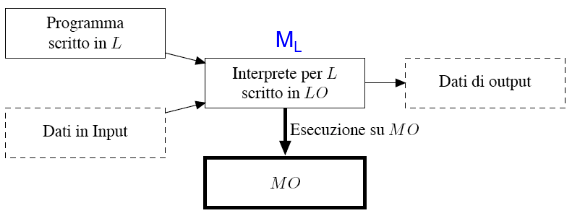
\includegraphics[width=0.5\textwidth]{img/interpretazione.png}
\end{center}
\textit{Definizione}: Un interprete per il linguaggio $\mathcal{L}$ scritto in $\mathcal{L}o$ è un programma che realizza una funzione parziale:
\begin{align*}
  I_\mathcal{L}^{\mathcal{L}o} \, : \, (P^\mathcal{L} \times D)-o \to D \\
  \text{tale che } I_\mathcal{L}^{\mathcal{L}o}(P_\mathcal{L}^{\mathcal{L}o}, \text{input}) = P^\mathcal{L}(\text{input})
\end{align*}
ove $P^\mathcal{L}$ indica un programma scritto in $\mathcal{L}$. \\
Quindi nella realtà l'interprete traduce riga per riga sul momento l'istruzione e l'esegue.
\subsection{Compilazione pura} 
I programmi in $\mathcal{L}$ sono \textbf{tradotti} in programmi in $\mathcal{L}o$: 
\begin{center}    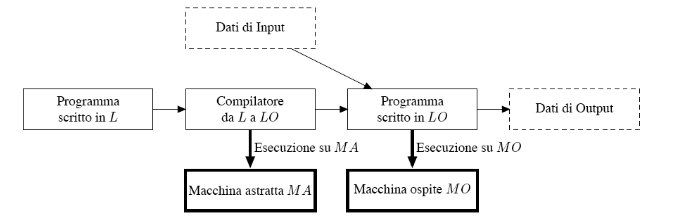
\includegraphics[width=0.5\textwidth]{img/compilazione.png}
\end{center}
Il compilatore scritto in $\mathcal{L}a$ tradude da $\mathcal{L}$ a $\mathcal{L}o$. Quindi prima traduciamo \texttt{tutto} e poi eseguiamo. \\
\textit{Definizione}: un compilatore da $\mathcal{L}$ a $\mathcal{L}o$ è un programma che realizza una funzione totale.
\begin{align*}
  C_{\mathcal{L},\mathcal{L}o} \, : \, P^\mathcal{L} \to P^{\mathcal{L}o}
\end{align*}
e quindi 
\begin{align*}
  P^\mathcal{L}(\text{input}) = P^{\mathcal{L}o}(\text{input})
\end{align*}
Definiamo \textbf{AOT} (ahead of time) la compilazione dove prima si traduce e poi si esegue.
\subsection{Compilazione o interpretazione?}
\begin{itemize}
  \item Interpretazione: \\
  - Debug facile \\
  - Più facile da creare
  - Lento (esecuzione + decodifica ogni riga ogni iterazione)
  \item Compilazione: \\
  - Perdita struttura del codice originale \\
  - Scarsa flessibilità \\
  - Più $\mathcal{L}$ è distante da $\mathcal{L}o$ più è lento. (ogni istruzione viene tradotta 1 sola volta + il carico della decodifica avviene sul compilatore)
\end{itemize}
Definiamo \textbf{JIT} (just in time) un mix tra compilazione e interpretazione. Un esempio è Java:
\begin{center}    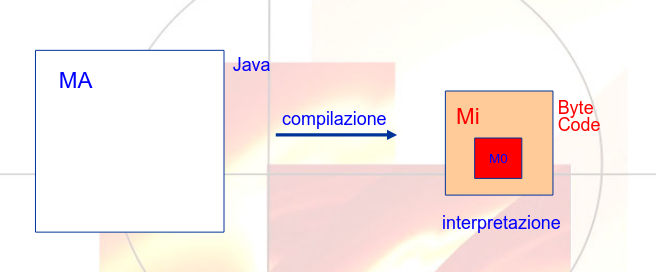
\includegraphics[width=0.5\textwidth]{img/java.png}
\end{center}
Dove Java ($\mathcal{L}_{MA}$) viene compilato in Bytecode ($\mathcal{L}_{Mi}$) che a sua volta viene compilato in codice macchina, mentre le funzioni vengono fatte dal interprete in JIT.
\section{Descrivere un linguaggio di programmazione}
Un linguaggio naturale/artificiale viene definito in 3 dimensioni:
\begin{itemize}
  \item Sintassi \\
  - Descrizione del lessico, ovvero le parole che posso utilizzare.
  \item Semantica \\
  - Per il lessico: Dizionari \\
  - Per le frasi: a quale lingua appartiene la frase, su quale linguaggio base (linguaggio da non spiegare) mi baso.
  \item Pragmatica \\
  - Implementare una frase sintatticamente corretta rispettando la sematica.
\end{itemize} 
Un linguaggio formale $L$ su alfabeto $A$ è un sottoinseme di $A^*$ ($L \subseteq A^*$), dove
\begin{align*}
  A* = U_{m \geq 0} \, A^n \text{ dove } A^0=\{\epsilon\}
\end{align*}
e 
\begin{align*}
  A^{n+1} = A \cdot A^n
\end{align*}
con 
\begin{align*}
  A \cdot A^n = \{aw \mid a \in A, \quad w \in A^n\}
\end{align*}
\textit{Osservazione}: $A^*$ è un insieme infinito contabile. 
\vspace{1em} \\
Dato un ordinamento del tipo $<$ (es. $a<b<c\dots$):
\begin{itemize}
  \item per primo abbiamo $\epsilon$ ($A^0$)
  \item poi elenco delle parole di $A^1$ ($a,b,c,\dots$)
  \item poi elenco delle parole di $A^2$ ($aa,ab,ac,\dots$)
\end{itemize}
\subsection{Notazioni}
\begin{itemize}
  \item Lunghezza: \\
  - $\mid \epsilon \mid$=0 \\
  - $\mid aw \mid = 1 + \mid w \mid $ \\
  - $\mid abc \mid = 3$
  \item Concatenazione: $x$ concatenato ad $y$ è la parola ottenuta sovrapponendo $x$ e $y$, ovvero $xy$\\
  $w=xy=\begin{cases} 
    \mid w \mid = \mid x \mid + \mid y \mid \\
    w(j)=x(j) \quad \text{ per } 1 \leq j \leq \mid x \mid \\
    w(\mid x \mid + j) = y(j) \quad \text{ per } 1  \leq j \leq \mid y \mid
  \end{cases}$ \\
  \textit{Nota}: $w(j)$ indica il j-esimo simbolo di $w$. \\
  \item Sottostringa: $\exists x,y \in A^*$ tale che $w=xy$ \\
  1) ogni stringa è sottostringa di se stessa \\
  2) $\epsilon$ è sottostringa di tutte le stringhe
  \item Suffisso: $V$ è suffisso di $w$ sse $\exists x \in A^*, w=xv$
  \item Prefisso: $V$ è prefisso di $w$ sse $\exists x \in A^*, w=vx$
  \item Potenza n-esima: \\
  - $w^0 = \epsilon$ \\
  - $w^{n+1} = ww^n \quad \forall n \geq 0$ \\
  Esempio: $(ab)^1=ab, \quad (ab)^2=abab$
  \item Linguaggio $L$ su alfabeto $A$: $L \subseteq A^*$ \\
  \begin{align*}
      L_1 = \{a,aa,\dots \}=\{a^n \mid n \geq 1 \} \\
      = A \setminus \{\epsilon\} \\
      = \{a^n \mid n \geq 0\}
  \end{align*}
\end{itemize}
\subsection{Operazioni sui linguaggi}
\begin{itemize}
  \item Completamento: $L^- = \{w \in A^* \mid w \notin L \}=A^* \setminus L$ \\
  \item Unione e Intersezione: \\
  - $L_1 \cup L_2 = \{w \mid w \in L_1 \text{ o } w \in L_2 \}$ \\
  - $L_1 \cap L_2 = \{w \mid w \in L_1 \text{ e } w \in L_2 \}$
  \item Concatenazione: ($\neq$ prodotto cartesiano) \\
  $L_1 \times L_2 = \{(w_1,w_2) \mid w_1 \in L_1 \text{ e } w_2 \in L_2\}$
  \item Chiusura / Stella di Kleene \\
  - $L^* = U_{n \geq 0} \, L^n$ \\
  - $L^+ = U_{n \geq 1} \, L^n$ (chiusura positiva)
\end{itemize}
\subsection{Rappresentazione finite dei linguaggi}
Se $L$ è infinito come possiamo rappresentarlo? (e come determiniamo una stringa $w \in L$) \\
\begin{itemize}
  \item Esempio 1: $N=\{1,2,3,\dots\}$ \\
   (Peano) $ o \in N, quad x \in N, quad S(x) \in N$ \\
   Genero: $\to \, N=\{o, S(o), S(S(o)), \dots \}$ 
  \item Esempio 2: $P=\{0,2,4,6,8,\dots \}$ \\
  Possiamo trovare una rappresentazione finita implicita. \\
  1) function \textit{pari} ($x$ : integer) $\to$ boolean \\
  2)   pari := (x mod 2 == 0) \\
  Riconosco se $x \in P$: Il programma è una rappresentazione finita implicita della funzione (infinita) che calcola.
\end{itemize}
Quindi abbiamo trovato 2 tecniche:
\begin{itemize}
  \item Generativo \\
  linguaggio = insieme delle stringhe generate da una struttura finita detta GRAMMATICA (a struttura di frase).
  \item Riconoscitivo \\
  linguaggio = insieme delle stringhe riconosciute da una struttura finita detta AUTOMA.
\end{itemize}
\textit{OSS}: Non tutti i linguaggi possono essere generati da grammatiche o riconosciuti da automi!
\subsection{Definire un linguaggio}
Esempio 1: Palindromo = parola che letta da sx a dx è uguale che da letta da dx a sx.
\begin{align*}
  A = \{a,b\} \\
  L = \{\epsilon, a, b, aa, bb, aba, bab, aaa, bbb, abba, baab, aaaa, bbbb, \dots \}
\end{align*}
Backus-Noun Form (\textbf{BNF}) \\
$<P> \, ::= \epsilon \mid a \mid b \mid a \, <P> \, a \mid b \, <P> \, b $\\ 
Ovvero: $<P>$ può essere le seguenti forme $\dots$ \\ 
\vspace{1em}
Come Grammatica: $P \to \epsilon \mid a \mid b \mid aPa \mid bPb$ \\
Definizione Ricorsiva: \begin{itemize}
 \item P è detto "simbolo non-terminale"
 \item a,b sono "simbolo terminale"
\end{itemize} 
Alternativamente: insieme degli assiomi e regole d'influenza. \\
$L(P)$ = "linguaggio generato a partire dal non-terminale P". E' il più piccolo insieme generato da questi assiomi e regole d'interferenza. \\
\vspace{2em} \\
Esempio 2: Espressioni aritmetiche formate a partire dalle variabili "$a$" e "$b$" con gli operatori "*", "+" e le parentesi (,). \\
Una \texttt{expr} può essere \begin{itemize}
  \item la variabile "a"
  \item la variabile "b"
  \item expr2 * expr2
  \item expr2 + expr2 
  \item (expr2)
\end{itemize}
BNF: 
\begin{align*}
  <E> ::= a \mid b \mid <E> * <E> \mid <E> + <E> \mid (<E>)
\end{align*}
Grammatica: 
\begin{itemize}
  \item $E \to a$
  \item $E \to b $
  \item $E \to E * E$
  \item $E \to E + E$
  \item $E \to (E)$
\end{itemize}
Brevemente: $E \to a \mid b \mid E * E \mid E+E \mid (E)$
\subsection{Come derivare una stringa?}
Dato: $P \to \epsilon \mid a \mid b \mid aPa \mid bPb$ \\
Si parte da $P$ e si applicano le produzioni. $P$ è palindromo perchè: \\
1)\begin{align*}
  P \to aPa \to abPba \to abba \text{ cioè } P \to *abba \\
  P \to aPa \, ; \, P \to bPb \, ; \, P \to \epsilon
\end{align*} 
2)\begin{align*}
  P \to bPb \to bbPbb \to bbabb \text{ cioè } P \to *bbabb \\
  P \to bPb \, ; \, P \to bPb \, ; \, P \to a
\end{align*} 
1.1) \begin{align*}
  \epsilon \in L(P) \\
  bb = b \epsilon b \in L(P) \\
  abba = ab \epsilon ba \in L(P)
\end{align*}
2.1) \begin{align*}
  a \in L(P) \\
  bab \in L(P) \\
  bbabb \in L(P)
\end{align*}
\subsection{Grammatiche}
\begin{itemize}
  \item Tante classi di grammatiche \\ 
  - regolari, libere (da contesto), dipendenti dal contesto, monotone, generali (o "a struttura di frase") 
  \item Tutte seguono lo stesso pattern, differenziandosi solo per come sono caratterizate le produzioni (o regole), ovvero le classificazioni di Chomsky)
  \item Quelle più utili sono le "libere"
\end{itemize}
\textit{Definizione}: una grammatica libera da contesto è una quadrupla (NT, T, R, S) dove 
\begin{itemize}
  \item NT è un insieme finito di simboli non-terminali (di solito lettere maiuscolo es. $A,B,C,\dots$)
  \item T è un insieme finito di simboli terminali (di solito lettere miniscole $a,b,c,\dots$)
  \item S $\in$ NT è detto simbolo iniziale 
  \item R è un insieme finito di produzioni (o regole) della forma \\
  $V \to w$ dove $V \in  NT$ e $w \in (N \cup NT)^*$
\end{itemize}
Esempio: 
\begin{align*}
  G = (\{S\}, \{a,b,+,*\}, S, R) 
\end{align*}
con 
\begin{align*}
  R = \{S \to_1 a, \\
  S \to_2 b, \\ 
  S \to_3 S+S, \\
  S \to_4 S*S \} \\
  \boxed{S \to a \mid b \mid S+S \mid S*S}
\end{align*}
\subsection{Derivazioni}
Dato $G=(NT,T,R,S)$ libera da contesto, diciamo che da $V$ si deriva immediatamente $w$ (o anche "$v$ si riscrive in un passo in più"), e lo denotiamo con $v \to w$, se
\begin{align*}
  v = \dfrac{xAy \quad (A \to z) \in R \quad w=xzy}{v \to w}
\end{align*}
con $x,y,z \in (T \cup NT)$. \\
Diciamo che $v$ si deriva da $w$ (o anche "$v$ si riscrive in $w$"), e lo denotiamo con $v \to^* w$, se esiste una sequenza finita (eventualmente vuota) di derivazioni immediate
\begin{align*}
v \to w_0 \to w_1 \to  w_1 \to \dots \to w
\end{align*}
cioè
\begin{align*}
  \dfrac{}{v \to^* w} \quad \dfrac{v \to^* w \, w \to z}{v \to^* z}
\end{align*}
"$\to^*$" è la chiusura riflessiva e transitiva della relazione "$\to$". \\
Esempio: 
\begin{align*}
  G \quad S \to a \mid b \mid S+S \mid S*S \\
  S+S \to S+S*S \to S+a*S \to S*S+a*S \\
  \text{cioè } S+S \to^* S*S+a*S
\end{align*}
\subsection{Linguaggio generativo}
\textit{Definizione}: Il linguaggio generato da una grammatica $G=(NT,T,R,S)$ è l'insieme 
\begin{align*}
  L(G)=\{w \in T^* \mid S \to^* w\}
\end{align*}
\textit{Spiegazione:} 
\begin{itemize}
  \item $w \in T^*$: solo terminali \\
  \item $S \to^* w$: si parte dal simbolo iniziale $S$
\end{itemize}
\vspace{1em}
Dato $G$, come faccio a determinare $L(G)$? Ed a verificare se $w \in L(G)$? 
\begin{itemize}
  \item attraverso tecniche opportune
  \item algoritmo \textit{naif}: \\
  - Parto da $S$ e provare ad applicare tutti i modi possibili le produzioni per trovare una derivazione che generi $w$
\end{itemize}
Esempio: \\
\begin{align*} 
  G_3 \quad S \to aSb \mid ab\\
  S \to_1 a \\
  \to_1 aSb \to_2 aabb \\
    \to_2 aaSbb \to_3 aaabbb \\
    \to_3 aaaSbbb
\end{align*}
è chiaro che $L(G_3)=\{a^nb^n \mid n \geq 1\}$. \\
Due grammatiche che generano lo stesso linguaggio si definiscono \textit{equivalenti}. \\
\begin{align*}
  G_2 \quad S \to AB \\
  A \to aA \mid a \\
  B \to bB \mid b \\
  L(G_2)=L(S)=L(A)\cdot L(B) \\
  = \{a^nb^m \mid n,m \geq 1 \}
\end{align*}
Ora al contrario dato un linguaggio come determiniamo una grammatica? \\
Esempio 1:
\begin{align*}
  L = \{a^nb^m \mid n \geq m \geq 0\} \\ 
  S \to AB \\
  A \to \epsilon \mid aA \\ 
  B \to aBb \mid \epsilon
\end{align*}
Esempio 2:
\begin{align*}
  L=\{a^{2n+1} \mid n \geq 0\} \\
  S \to a \mid aaS \\
  =\{a, aaa, aaaaa, \dots\}
\end{align*}
Esempio 3:
\begin{align*}
  L=\{a^{2n}b^{2m+1} \mid n,m \geq 0\} \\
  S \to aaS \mid bB \\
  B \to \epsilon \mid bbB
\end{align*}
Esempio 4 (linguaggio finito):
\begin{align*}
  S = \{ab, ac, ad \} \\
  S \to ab \mid ac \mid ad \\
  \text{oppure} \\
  S \to aA \\
  A \to b \mid c \mid d
\end{align*}
\section{Derivazioni ed alberi}
consideriamo le grammatiche $S \to a \mid b \mid c \mid S+S \mid S*S$, consideriamo la derivazione
\begin{align*}
  S \to S*S \to S+S*S \to a+S*S \to a+b*S \to a+b*c
\end{align*}
\begin{itemize}
  \item leftmost: ad ogni passo riscriviamo il nonterminale più a sx.
  \item è possibile associare un albero di derivazione
 \begin{center}    
\includegraphics[width=0.35\textwidth]{img/albero.png}
\end{center}
\end{itemize}
Osservazioni:
\begin{itemize}
  \item Un albero di derivazione riassume tante derivazioni diverse ma tutte equivalenti
  \item Esiste una corrispodenza biunivoca tra derivazioni canoniche sinbistre (o destre) e alberi di derivazione.
  \item L'albero di derivazione fornisce informazioni semantiche: "quali operandi per quali operatori". 
   \begin{center}    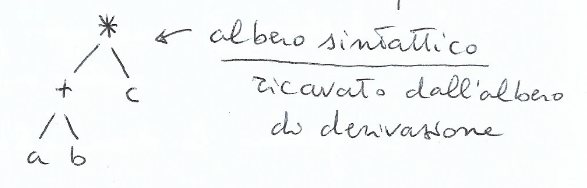
\includegraphics[width=0.5\textwidth]{img/albero_sintattico.png}
\end{center}
\end{itemize}
\subsection{Albero di Parsing}
Data una grammatica $G=(NT,T,S,R)$ un albero di parsing (o derivazione) è un albero ordinato:
\begin{itemize}
  \item ogni nodo è itechettato con simboli in $NT \cup \{\epsilon\} \cup T$
  \item la radice è etichettata con S
  \item ogni nodo è itechettato con un simbolo in NT
  \item se il nodo $n$ ha etichetta $\epsilon$ allora $n$ è una foglia figlio unico con A come padre
  \item ogni nodo foglia è itechettato su $T \cup \{\epsilon\}$ allora l'albero corrisponde ad una derivazione completa
\end{itemize}
\subsection{Ambiguità}
Consideriamo
\begin{align*}
  S \to a \mid b \mid c \mid S+S \mid S*S
\end{align*}
ha due derivazioni leftmost per $a*b+c$:
\begin{itemize}
  \item 1) $S \to S+S \to S*S+S \to a*S+S \to a*b+S \to a*b+c$
  \item 2) $S \to S*S \to a*S \to a*S+S \to a*b+S \to a*b+c$
\end{itemize}
Avendo più grammatiche, la stringa "$a*b+c$" ha più di un albero di derivazioni. Quindi la grammatica non è unica, è ambigua. \\
Prendiamo in considerazione la grammatica:
\begin{itemize}
  \item $E \to E + T \mid T$ \\
  \item $T \to A*T \mid A $\\
  \item $A \to a \mid b \mid c$ \\
\end{itemize}
. \\
\begin{center}    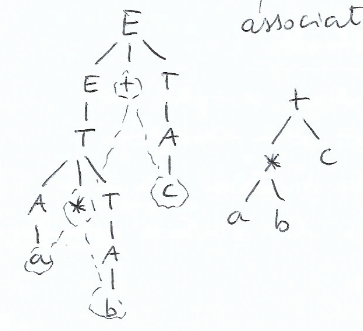
\includegraphics[width=0.3\textwidth]{img/albero_sintattico2.png}
\end{center}
Notiamo come non sia possibile fare "$a* \, b\text{+}c$"! \\
Per risolvere possiamo ottenere (quasi) lo stesso linguaggio con gli stessi laberi sintattici possiamo: \\
\begin{itemize}
  \item $E \to E + T \mid T$ \\
  \item $T \to A*T \mid A $\\
  \item $A \to a \mid b \mid c \mid (E)$ \\
\end{itemize} 
.
\begin{center}    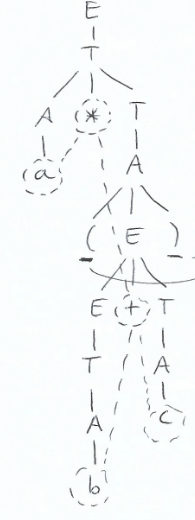
\includegraphics[width=0.15\textwidth]{img/albero_sintattico3.png}
\end{center}
Le parentesi sono \texttt{zucchero sintattico}. Ora possiamo avere anche espressioni come "$a*(b+c)$"! \\
\vspace{2em}\\
Ora consideriamo la grammatica: 
\begin{align*}
  \langle stm \rangle &::= \text{if } \langle expr \rangle \text{ then } \langle stm \rangle \\
  &\mid \text{if } \langle expr \rangle \text{ then } \langle stm \rangle \text{ else } \langle stm \rangle \\
  &\mid \dots
\end{align*}
Pero questa sintassi è ambigua!
\subsection{Grammatica concreta}
\begin{align*}
  \langle stm \rangle &::= \langle matched\text{-}stm \rangle \mid \langle unmatched\text{-}stm \rangle
\end{align*}
\begin{align*}
  \langle matched\text{-}stm \rangle &::= \text{if } \langle expr \rangle \text{ then } \langle matched\text{-}stm \rangle \text{ else } \langle matched\text{-}stm \rangle \\
  &\mid \text{begin } \langle stm \rangle \text{ end} \\
  &\mid \dots
\end{align*}
\begin{align*}
  \langle unmatched\text{-}stm \rangle &::= \text{if } \langle expr_2 \rangle \text{ then } \langle stm \rangle \\
  &\mid \text{if } \langle expr_1 \rangle \text{ then } \langle matched\text{-}stm \rangle \text{ else } \langle unmatched\text{-}stm \rangle \\
  &\mid \dots
\end{align*}
Così abbiamo una sintassi non ambigua!
\section{Variabili sintattici contestuali}
Esempi: 
\begin{itemize}
  \item una variabile deve essere dichiarata
  \item compatibilità di assegnamento di tipo
  \item numero e tipo di parametri di una funzione passati (parametro attuale) devono essere uguali al tipo dichiarato dalla funzione (parametro formale).
\end{itemize}
Queste formano vincoli sintattici, non sono esprimibili da grammatiche libere (BNF) perchè questi non possono definire vincoli. Che soluzioni abbiamo?
\begin{itemize}
  \item Con strumenti più potenti, con \textit{grammatiche dipendenti da contesto}
  \item Con controlli "ad hoc". Ovvero una analisi semantica per i controlli sintattici contestuali
\end{itemize}
\paragraph*{Sintassi o Semantica?\\}
La sintassi è ciò che descrive una BNF (per le grammatiche libere), il resto è semantica. Quindi i vincoli contestuali appartengono alla semantica. Il compilatore, alla terza fase, fa la analisi semantica. \\
\begin{itemize}
  \item Semantica statica: insieme dei controlli fatti sul testo del programma (es. \textit{type checking})
  \item Semantica dinamica: rappresentazione formale durante l'esecuzione del programma (es. divisione per 0) \\
  - Modello matematico che descrive il "comportamento" del programma.
\end{itemize}
Soffermiamoci sulla semantica dinamica
\begin{itemize}
  \item Al programmatore: \\
  - deve sapere cosa sta facendo il programma   \\
  - deve poter dimostrare le proprietà del suo programma (es. termina sempre con qualsiasi input?)
  \item Al progettista del linguaggio: \\
  - strumento di specifica del linguaggio \\ 
  - deve poter dimostrare proprietà del linguaggio (è Tuning-completo?)
  \item All'implementazione del linguaggio: \\
  - dimostrare la correttezza dell'implementazione
\end{itemize}
Un compilatore controlla la semantica statica, però è completo quando \textbf{preserva la semantica dinamica}. \\
\subsection{Come si fa a definire la semantica?}
\begin{itemize}
  \item Operazionale: \\
  - un autonoma che passo passo mostra l'effetto della esecuzione delle istruzioni, ci si sofferma su \texttt{come si calcola}
  \item Denotazionale: (non lo vedremo)\\
  - ad ogni programma si associa un funzione input/output, ci si sofferma su \texttt{come si calcola} 
  \item (+) Pragmatica: regola e consigli su come è meglio utilizzare le istruzioni
\end{itemize}
\paragraph{Implementazione\\}
Scrivere un compilatore (o interprete) per una macchina ospite (già realizzata) così costruendo una macchina astratta. \\
\vspace{1px}\\
- Correttezza del compilatore? Preserva la semantica? (Il programma sorgente e quello oggetto calcolano la stessa funzione?) \\
- Costo della compilazione? 
\begin{center}
    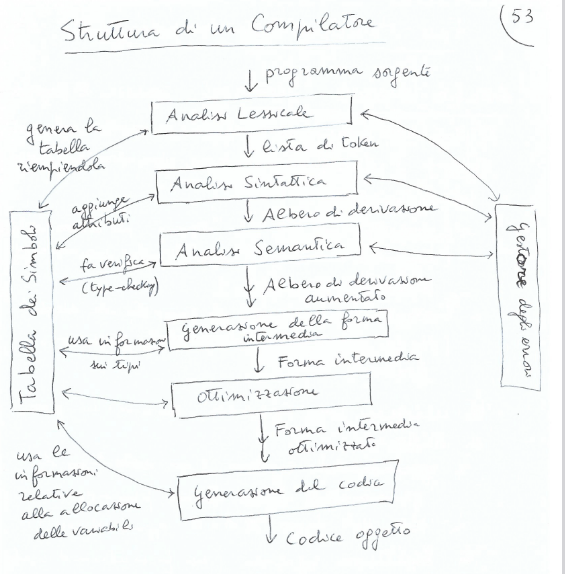
\includegraphics[width=0.9\textwidth]{img/compilatore.png}
\end{center} 
Gli errori rilevati nelle prime 3 fasi non bloccano il compilatore ma genera un messaggio di errore! Alla fine della terza fase se ci sono errori si blocca e printa gli errori, se NON ci sono errori genera una forma "intermedia" del codice NON OTTIMIZZATA; la ottimizza e poi da li genera il codice oggetto.
\subsection{Fasi di un compilatore}
\begin{itemize}
  \item Analisi lessicale (Scanner) \\
  - spezza il codice sorgente in \textbf{tokens} ciò in identificatori, numeri, operatori, parentesi, parole riservate, $\dots$. Riempe la tabella dei simboli + parametri aggiuntivi \\
  - controlla che la grammatica sia regolae ($A \to aB$ o $A \to a$) \\
  - espressioni regolari \\
  - automi a stati finiti (NFA - DFA)
  \item Analisi sintattica (Parser) \\
  - prende in input la lista dei token (dello scanner) e genera l'albero sintattico, controlla le espressioni artimetiche \\
  - verifica che i comandi sia composti secondo le regole grammaticali
  \item Analisi semantica \\
  - esegue controlli di semantica statica (ovvero sintattici contestuali) per rilevare errori semantici (es. tipi, parametri formali vs attuali, ecc)\\
  - arricchisce albero del parsec con i tipi
  \item Generazione forma intermedia \\
  - genera un codice scritto in linguaggio intermedio indipendente dall'architettura (facilmente traducibile in tutti i linguaggi) \\
  - si segue la struttura dell'albero sintattico ricavato dall'albero di derivazione
  \item Ottimizzazione \\
  - si effettuano ottimizzazioni su codice intermedio (rimozione codice inutile, mettere fuori da cicli operazione che non variano, ecc)
  \item Generazione del codice \\
  - generiamo il codice di una specifica architettura (include anche assegnazione dei registri e ottimizzazione specifiche per quall'architettura)
  \item Tabella dei simboli \\
  - memorizza le informazioni sui nomi presenti nel programma (identificatori di variabile, funzioni, procedure, ecc)
\end{itemize}
\section{Semantica operazionale strutturale}
\begin{itemize}
  \item Linguaggio
  \begin{itemize}
    \item definito tramite sintassi astratta
    \item ad ogni stringa viene accoppiato un albero sintattico (non ambiguo)
  \end{itemize}
  \item Insiemi di base
  \begin{itemize}
    \item booleani 
    \item numeri naturali
    \item variabili
  \end{itemize}
  \item Insiemi derivati
  \begin{itemize}
    \item Espressioni aritmetiche $e \in Exp$ \\
    \begin{align*}
      e ::= m \mid \text{v} \mid e+e \mid e-e \mid e*e 
    \end{align*}
    \item Espressioni booleane $b \in Bxp$
    \begin{align*}
      b ::= t \mid e=e \mid b \text{ or } b \mid \sim b
    \end{align*}
    \item Comandi $c \in Com$
    \begin{align*}
      c ::=  \text{ skip }\mid v ::= e \mid c;c \mid while \, b \, do\,  c \mid if \, b \, then \, c \, else \, c
    \end{align*}
  \end{itemize}
\end{itemize}
Infatti Parser(programma scritto insintassi concreta) $\to$ Albero sintattico di sintassi astratta \\
\subsection*{Come dare semantica?}
Definiamo per ogni categoria sintattica (Exp, Bex, Com) un modello detto "sistema di transizione". Un sistema di transizione è una tuple $\langle \Gamma, \top, \to \rangle$ dove
\begin{itemize}
  \item $\Gamma$ è l'insieme (anche infinito) degli stati
  \item $\top \subseteq \Gamma$ è l'insieme degli stati terminali
  \item $\to \subseteq \Gamma \times \Gamma$ è la relazione di transizione
\end{itemize}
- Una computazione a partire dallo stato $y_0$ è una sequenza $y_0 \to y_1 \to \dots $ che può essere finita o infinita. \\
- Con $\to^*$ indichiamo la chiusura riflessiva e transitiva di $\to$, ovvero:
\begin{align*}
  \dfrac{}{y \to^* y} \quad \dfrac{y \to^* y' \, y'\to y''}{y \to^* y''}
\end{align*}
\begin{center}    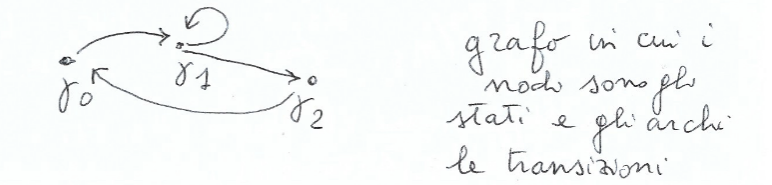
\includegraphics[width=0.5\textwidth]{img/grafo.png}
\end{center}
\begin{itemize}
  \item $\Gamma$ essendo spesso infinito dobbiamo trovare una rappresentazione finita implicita attraverso una BNF
  \item $\to \subseteq \Gamma \times \Gamma$ essendo una relazione infinita costituita da coppie $y \to y'$ neccessita di trovare una rappresentazione finita implicita come minima relazione che soddisfa un certo insieme di assiomi e regole di interferenza.
  \item Per dare significato alla variabili è necessario introdurre uno \textbf{store} $\sigma : Var \to N$
\end{itemize} 
Vediamo ora:
\begin{align*}
  \langle \Gamma_e, \top_e, \to_e \rangle
\end{align*}
dove
\begin{itemize}
  \item $\Gamma_e = \{\langle e, g \rangle \mid e \in Exp, \sigma \in Store\}$ 
  \item $\top_e = \{\langle n, g \rangle \mid n \in N, \sigma \in Store\}$
  \item la relazione $\to_e$ è definita come la minima relazione che soddisfa gli assiomi e le regole di interferenza qui sotto:
  \begin{center}    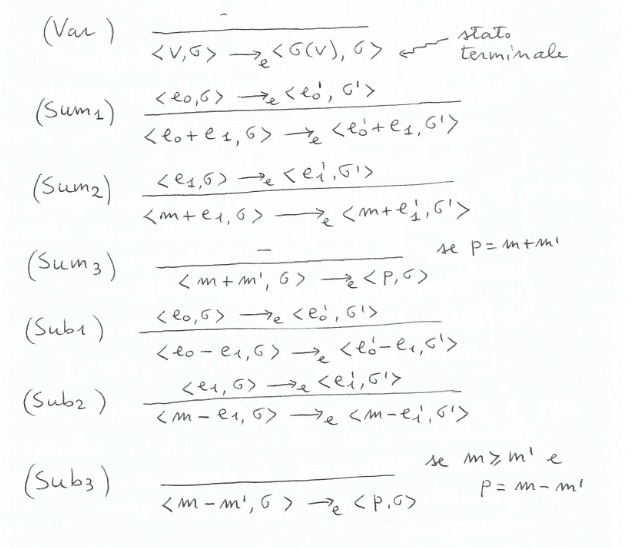
\includegraphics[width=0.8\textwidth]{img/regole.png}
\end{center}
\end{itemize}
Osservazioni:
\begin{itemize}
  \item Gli assiomi e le regole SOS sono facilemente implementabili in Prolog, con un semplice ma inefficiente interprete per le espressioni aritmetiche
  \item Lo store $\Gamma$ non viene mai modificato durante la valutazione di una espressione!
  \item La regola Sum1 e Sum2 riflettono una regola di valutazione IS (interna sinistra)
  \begin{itemize}
    \item prima valutiamoargomento a sx
    \item quando abbiamo finito si valuta il secondo 
    \item si fa la somma (Sum3)
  \end{itemize}
\vspace{5em}
\end{itemize}
\begin{center}    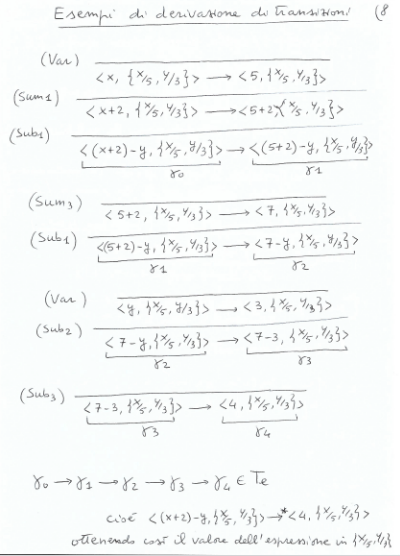
\includegraphics[width=0.6\textwidth]{img/esempi2.png}
\end{center} 
\subsection{Induzione strutturale}
Vogliamo dimostrare un proprieta $P(e)$ per ogni $e \in Exp$
\begin{center}    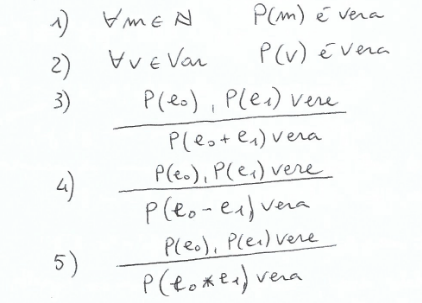
\includegraphics[width=0.3\textwidth]{img/dimostrazione.png}
\end{center}
allora concludiamo che $\forall e \in Exp \quad P(e)$ è vera. Dimostrazione in "Lez05-Gorrieri.pdf" pagine 10/11. Qed. \\
Poichè $\to_e$ è deterministica a partire da $\langle e, \sigma\rangle$ arriveremo ad una sola configurazione terminale $\langle n, \sigma \rangle$: "n è il valore di $e$ in $\sigma$. È possibile definire una funzione:
\vspace{8em}
\begin{center}    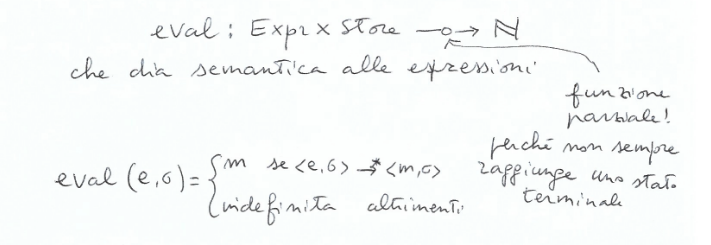
\includegraphics[width=0.8\textwidth]{img/func.png}
\end{center}
Vediamo qualche esempio:
\begin{center}    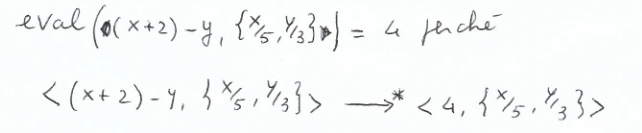
\includegraphics[width=0.5\textwidth]{img/esempio3.png}
\end{center}
\vspace{2em}
Eval è definita rispetto alla disciplina di valutazione IS. A rigore $eval_{IS}$.
\subsection{Semantica delle espressioni booleane}
\begin{align*}
  b ::= t \mid e=e \mid b \text{ or } b \mid  \sim bbbbbbbbbbbbbbbb 
\end{align*}
\begin{align*}
\langle \Gamma_{b'}, \top_{b'}, \to_b \rangle \text{ dove } \\
1) \, \Gamma_b = \{\langle b, \sigma \rangle \mid b \in Bexp, \sigma \in Store \} \\
2) \, \top_b = \{\langle tt, \sigma \rangle, \langle ff, \sigma \rangle, \langle \sigma \in Store \rangle \}
\end{align*}
$e \to_b $ è la minima relazione generata dai seguenti assiomi e regole d'interferenza
\begin{center}    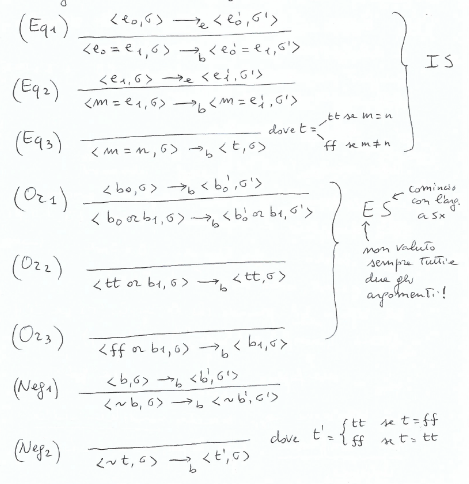
\includegraphics[width=0.5\textwidth]{img/regole2.png}
\end{center}
Osservazione
\begin{itemize}  
  \item lo store $\sigma$ non viene mai modificato
  \item $\to_b$ è deterministica (se $y \to_b y'$ e $y \to_b y''$ allora $y'=y''$)
\end{itemize}
\subsection{Semantica dei comandi}
\begin{align*}
  c ::= skip \mid v := e \mid c;c \mid if \, b \, then \, c \, else \, c \mid while \, b \, do \, c
\end{align*}
\begin{align*}
  \langle \Gamma_c, \top_c, \to_c \rangle \text{ dove } \\
  1) \, \Gamma_c = \{\langle c, \sigma \rangle \mid c \in Com, \sigma \in Store \} \cup \{\sigma \mid \sigma \in Store\}\\
  2) \, \top_c = \{\sigma \mid \sigma  \in Store\}
\end{align*}
$e \to_c \subseteq \Gamma_c \times \Gamma_c$ è la più piccola relazione generata dai seguenti assiomi e regole di interferenza.1
\begin{center}    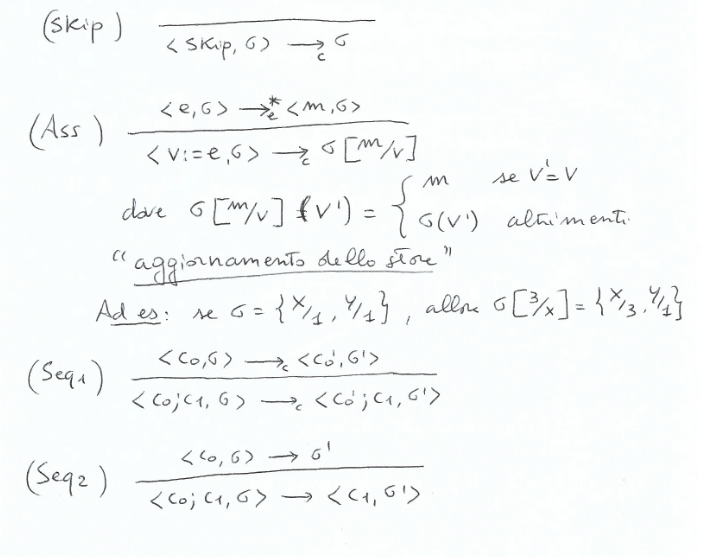
\includegraphics[width=0.5\textwidth]{img/comandi1.png}
\end{center}
\begin{center}    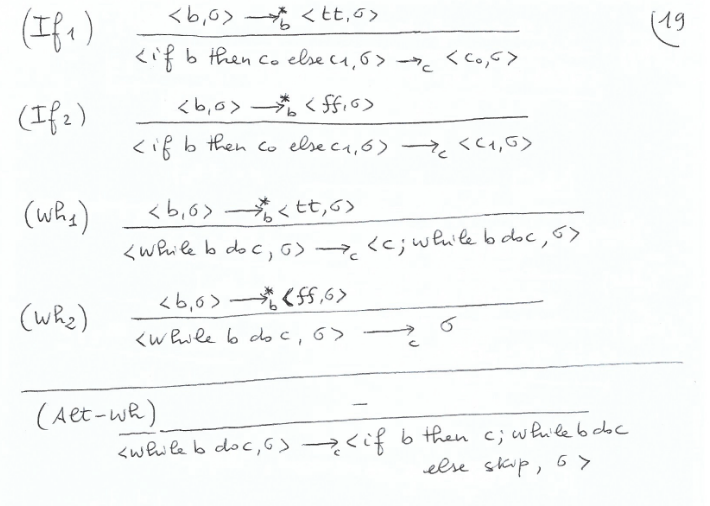
\includegraphics[width=0.5\textwidth]{img/comandi2.png}
\end{center}
\subsection{Errori dinamici (a runtime)}
\begin{align*}
\Gamma'=\Gamma \cup \{ err \} \quad T'=T \cup \{ err \} \\
eval \, : \, Exp \times Store \to_{\text{totale}} N \cup \{err\} \\
eval_b \, : \, Bexp \times Store \to \top\top \cup \{ err \} 
\end{align*}
\begin{align*}
exec \, : \, Com \times Store \to_o Store \cup \{err\} \quad \text{(rimane parziale per runtime)}
\end{align*}
\subsection{Nondeterminismo e Parallelismo}
\begin{align*}
c ::= skip \mid v:= e \mid \dots \mid c \text{ or } c \mid c \text{ par } c
\end{align*}
Scelgo un comando e "butto via" l'altro.
\begin{center}    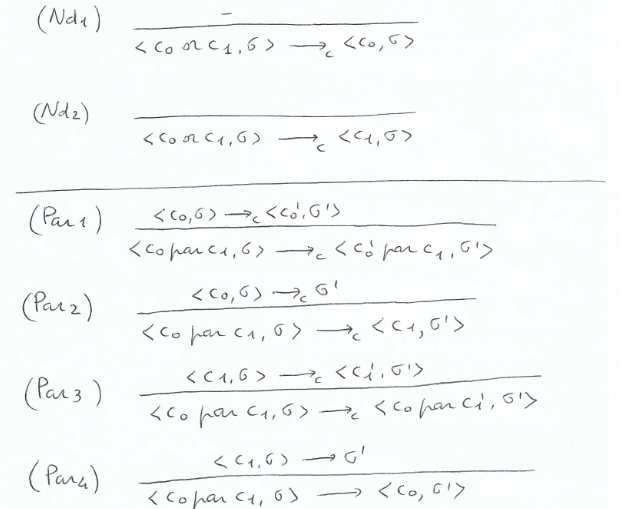
\includegraphics[width=0.5\textwidth]{img/non_par.png}
\end{center}
Verificare che $\to_c$ non è più determinanistico sul linguaggio esteso con "or" e "par". Per farlo vedere costriuamo il sistema di transizione per $(x:=0; \, x:=x+1)$ per $x:=1$
\begin{center}    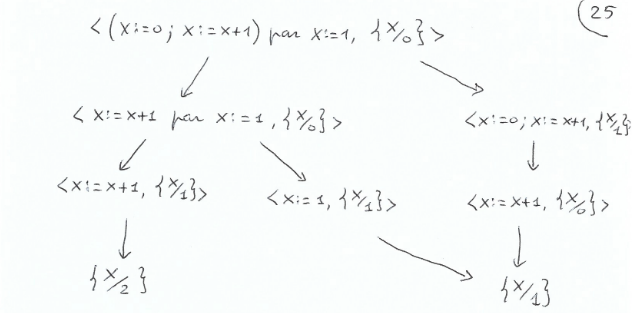
\includegraphics[width=0.5\textwidth]{img/esempio4.png}
\end{center}
\begin{itemize}
  \item Due possibili risultati finali: $\{x/1\}$ o $\{x/2\}$
  \item Per modellare questa situazione
  \begin{align*}
    exec : Com \times Store \to_o P(Store) \\
    exec((x:=0; x:=x+1) \text{ per } x:=1, \{x/0\}) = \{\{x/1\},\{x/2\} \}
  \end{align*}
\end{itemize}
Possiamo ampliare l'errore dinamico con
\begin{center}
    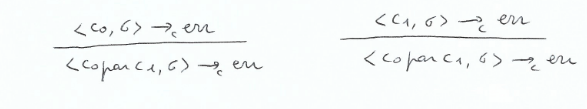
\includegraphics[width=0.7\textwidth]{img/errore_dinamico.png}
\end{center} 
\section{Analisi Lessicale - linguaggi regolari}
\textit{Analisi lessicale}: riconoscere nella stringa in ingresso sequenze di simboli che corrispondono a specifiche categorie sintattiche (token).
\begin{align*}
\text{Programma in input} \to \text{\boxed{Analizzatore \quad lessicale} (scanner)} \to \text{lista di token}
\end{align*}
Cosa è un \texttt{token}? É una coppia (nome, valore). Ad ogni nome di categoria è associato un "pattern" che specifica i possibili "valori" che possono essere presi per quel nome, come "lessemi".
\begin{center}
    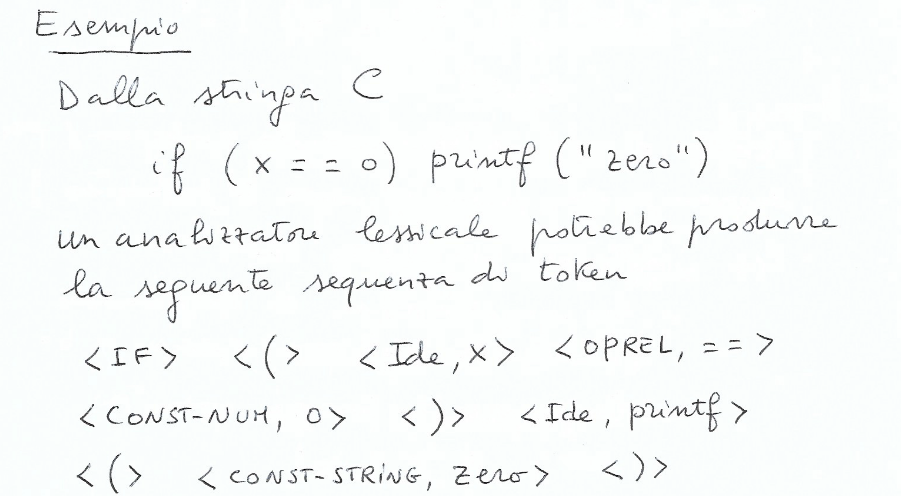
\includegraphics[width=0.7\textwidth]{img/c.png}
\end{center} 
\subsection{Espressioni regolari}
Fissato un alfabeto $A=\{a_1,a_2,\dots,a_n\}$ definiamo le espressioni regolari su $A$ con le seguenti BFN
\begin{align*}
r ::= \emptyset \mid \epsilon \mid a (\forall a \in A) \mid r \cdot r \mid r|r \mid r*
\end{align*}
Questa è una sintassi astratta ambigua, per disambiguare dobbiamo aggiungere le parentesi.
\subsection{Linguaggio denotato da una espressione regolare}
Dato l'alfabeto $A$ definiamo la funzione 
\begin{align*}
L : Exp-Reg \to P(A*)
\end{align*}
come segue
\begin{itemize}
  \item $L[\emptyset]= \emptyset$ (linguaggio vuoto)
  \item $L[\epsilon]=\{\epsilon\}$ (linguaggio con una sola stringa quella vuota)
  \item $L[a]=\{a\}$
  \item $L[r_1 \cdot r_2] = L[r_1] \cdot L[r_2] $
  \item $L[r_1 \mid r_2] = L[r_1] \cup L[r_2] $
  \item $L[r*]=(L[r])* $
  \item Se si utilizzano le parentesi: $L[(r)] = L[r]$
\end{itemize}
\subsection*{Linguaggio Regolare}
Un linguaggio regolare $L \subseteq A*$ è detto regolare sse esiste una espressione regolare $r$ tale che $L = L[r]$. Ogni linguaggio finito è regolare, ma esistono linguaggi regolai infiniti. \\
\vspace{1em}
Una definizione regolare su alfabeto A è costituita da una lista di definizioni
\begin{align*}
d_1 := r_1 \\
d_2 := r_2 \\
\vdots \\
d_k := r_k
\end{align*}
dove i vari $d_i$ sono simboli nuovi e ogni $r_i$ è una espressione regolare sull'alfabeto esteso $A \cup \{d_1, d_2, \dots , d_k \}$.
\begin{center}
    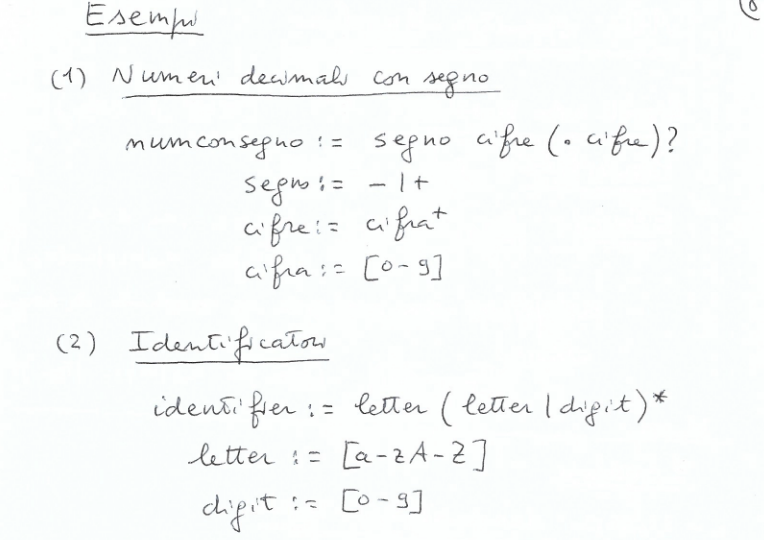
\includegraphics[width=0.7\textwidth]{img/esempio5.png}
\end{center} 
\subsection{Equivalenza tra espressioni regolari}
Due espressioni regolari $r$ e $s$ sono equivalenti sse $L[r]=L[s]$ (ovvero denotano lo stesso linguaggio) e lo denotiamo come $r \simeq s$. Le espressioni regolari servono per specificare il pattern di una categoria sintattica, ovvero la forma dei possibili lessemi.
\subsection{Automi (a stati) finiti}
Come facciamo a riconoscere se una sequenza in ingresso è un lessema per una categoria sintattica? Con gli automi a stati finiti!
\begin{center}
    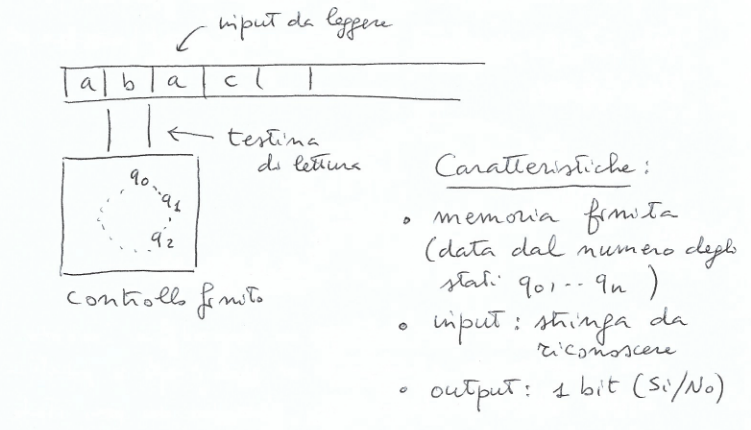
\includegraphics[width=0.5\textwidth]{img/automi_finiti.png}
\end{center} 
\begin{itemize}
  \item Descrizione iniziale
    \begin{itemize}
    \item lettura posizionale a partire dal primo carattere 
    \item controllo su stato iniziale $q$
  \end{itemize}
  \item Funzionamento: \textit{Ripeti}
    \begin{itemize}
    \item leggi il carattere in input in base allo stato decidiamo poi: \\
    cambiare stato  \\
    spostare input seccessivo finchè:
        \begin{itemize}
       \item finito di leggere input 
      \item oppure fermato perchè non specificato uno stato successivo
    \end{itemize} 
  \end{itemize}
\end{itemize}
\subsection*{Diagrammi di transizione}
Il funzionamento di un automa finito è ben rappresentato attraverso un diagramma di transizione
\begin{center}    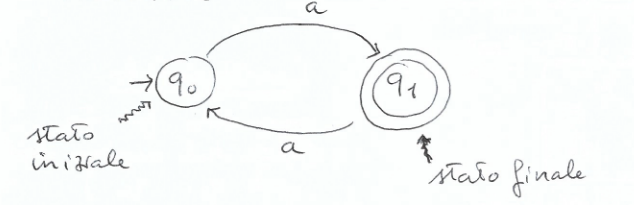
\includegraphics[width=0.5\textwidth]{img/transizione.png}
\end{center}
Riconoscere una stringa significa trovare un cammino eticchettato sul grafo a partire dello stato iniziale che finisce su uno stato finale 
\begin{align*}
  L = \{a^{2n+1} \mid n \geq 0\}\ = \{ a^n \mid n \text{ è dispari }\} \\
  = L[a(aa)*]
\end{align*}
\begin{center}    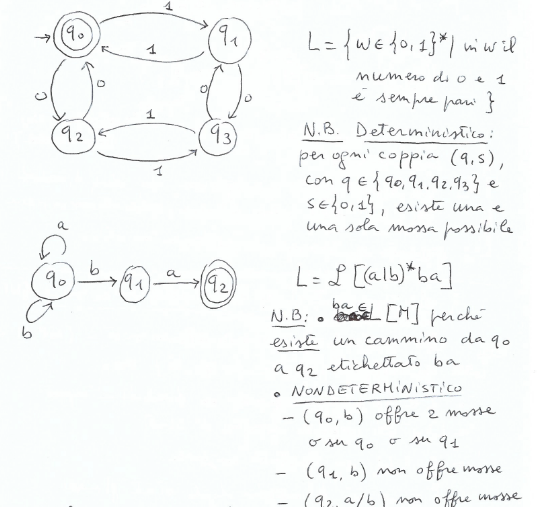
\includegraphics[width=0.5\textwidth]{img/esempio6.png}
\end{center}
\subsection{Automi finiti nondeterministici}
Un automa finito nondeterminismo (NFA) è una quintupla $\{\sum, Q, \delta, q_0, F\}$ dove
\begin{itemize}
  \item $\sum$ è un alfabeto finito di simboli in input
  \item $Q$ è un insieme finito di stati
  \item $q_o \in Q$ è lo stato iniziale
  \item $F \subseteq Q$ è l'insieme degli stati finali
  \item $\delta$ è la funzione di transizione con tipo 
  \begin{align*}
    \delta : Q \times (\sum \cup \{ \epsilon\}) \to P(Q) \text{ (insieme delle parti di Q)}
  \end{align*}
  \begin{align*}
    (\delta(q, \sigma)= Q' \subseteq Q)
  \end{align*}
\end{itemize}
Vediamo un esempio
\begin{center}    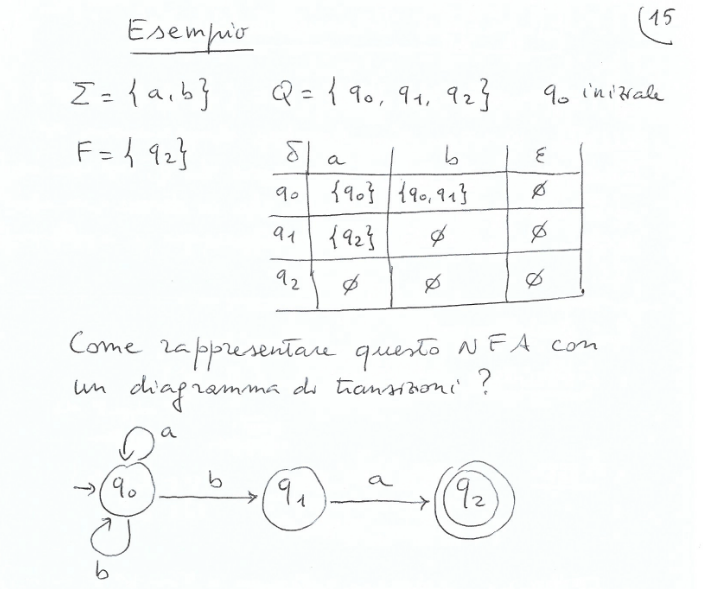
\includegraphics[width=0.7\textwidth]{img/esempio7.png}
\end{center}
\subsection{Linguaggio riconosciuto / accettato}
Un NFA $N=\{\sum, Q, \delta, q_0, F\}$ accetta $w=a_1,\dots,a_n$ sse nel diagramma di transizione esiste un cammino da $q_0$ ad uno stato in $F$ nel quale la stringa che si ottiene concatenando le etichette degli archi percorsi è esattamente $w$.
\vspace{9em}
\begin{center}    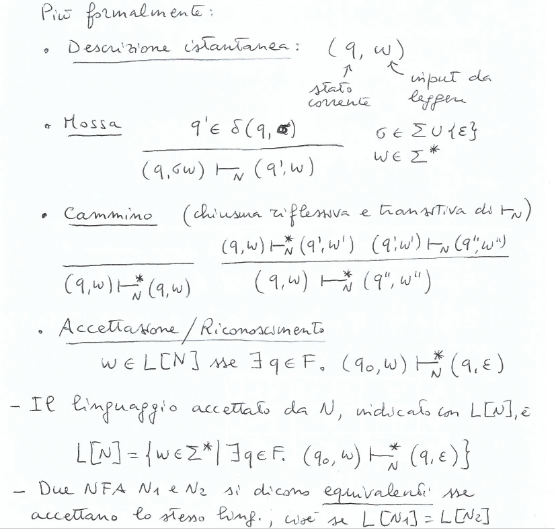
\includegraphics[width=0.7\textwidth]{img/esempio8.png}
\end{center}
Esempio: \\
Costruire un NFA per il linguaggio $L_1 = \{a^n b^m \mid n,m \geq 1 \}$
\begin{center}    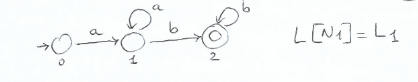
\includegraphics[width=0.8\textwidth]{img/esempio9.png}
\end{center}
Quindi ricapitolando
\begin{itemize}
  \item NFA: sono comodi, facili ma inefficienti (tante strade se un grafo)
  \item DFA: $\delta(q, \sigma)$ è sempre un singoletto, solo una mossa possibile. Non ci sono le mosse $\epsilon$. Non si blocca mai, fa la scansione completa del input. Più diffice da definire.
\end{itemize}
\subsection{Automi finiti deterministici}
Un DFA è una quintupla $(\sum, Q, \delta, q_0, F)$ dove $\sum, Q, q_0$ e $F$ sono definiti come per una NFA, mentra la funzione di transizione $\delta$ ha tipo
\begin{align*}
  \delta : Q \times \sum \to Q \\
  (\delta(q, \sigma)=q')
\end{align*}
Si può notare che una DFA è un particolare tipo di NFA tale che 
\begin{itemize}
  \item $\forall q \in Q \quad \delta(q, \epsilon)= \emptyset$ (non ci sono transizioni $\epsilon$)
  \item $ \forall \sigma \in \sum, \forall q \in Q, \exists q' \in Q. \quad \delta (q, \sigma) = \{ q' \}$ (l'insieme delle mosse possibili è sempre un singoletto).
\end{itemize}
quindi DFA $\subset$ NFA. \\
Vogliamo ora dimostrare che i DFA sono tanto espressivi quanto gli NFA sebbene siano un sottoinsieme proprio degli NFA. Idea: seguire contemporaneamente tutti i possibili cammini alternativi dell'NFA. Ovvero gli stati del DFA che andiamo a costruire sono costituiti da insieme di stati dell'NFA.
\begin{center}
    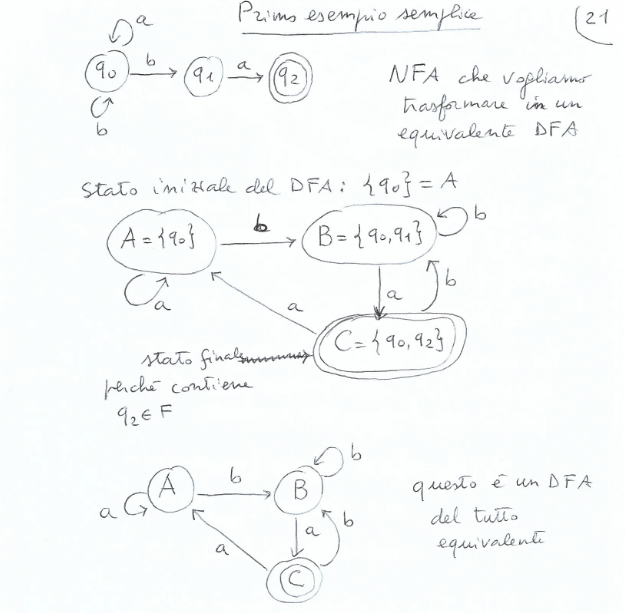
\includegraphics[width=0.7\textwidth]{img/esempio10.png}
\end{center} 
\begin{itemize}
  \item Passando dallo stato $A=\{q_0\}$ allo stato $B=\{q_0, q_1\}$, ho seguito contemporaneamente tutte le due transizioni etichettate $b$
  \item Passando dallo stato $B=\{q_0, q_1\}$ a $C=\{q_0, q_2\}$, ho seguito sia la transazione $q_0 \to_a q_0$ sia la transazione $q_1 \to_a q_2$
\end{itemize}
\begin{align*}
  mossa(B, a) = \bigcup_{q \in B} \delta(q, a) \\
  = \delta(q_0, a) \cup \delta(q_1, a) \\
  = \{q_0, q_2 \} \\
  = C
\end{align*}
\begin{center}
    
\includegraphics[width=0.7\textwidth]{img/es2.png}
\end{center} 
Lo \textit{stato iniziale} del DFA è dato da $o$, più tutti gli stati che possono raggiungere da $o$ con mossa $\epsilon$
\begin{align*}
  \epsilon\text{-closure($o$)} = \{ 0, 1, 2, 3, 7\} \quad (A)
\end{align*}
Per calcolare lo stato che raggiungo da $A$ leggendo "$a$", devo vedere quali stati in $A$ possono fare $a$ e poi fare la $\epsilon$-closure
\begin{align*}
  \triangle (A, a) = \epsilon\text{-closure}(mossa(A, a)) \\
  = \epsilon\text{-closure}(\bigcup_{q \in A} \delta(q, a)) \\
  = \epsilon\text{-closure}(\{4\}) \\
  = \{4, 6, 7, 1, 2, 3\} \\
  = B
\end{align*}
\begin{align*}
  \triangle (A, b) = \epsilon\text{-closure}(mossa(A, b)) \\
  = \epsilon\text{-closure}(\bigcup_{q \in A} \delta(q, b)) \\
  = \epsilon\text{-closure}(\{5, 8\}) \\
  = \{1, 2, 5, 6, 7, 8\} \\
  = C
\end{align*}
\begin{align*}
  \triangle (B, a) = \epsilon\text{-closure}(\{4\}) \\
  = B 
\end{align*}
\begin{align*}
  \triangle (B, b) = \epsilon\text{-closure}(\{5, 8\}) \\
  = C 
\end{align*}
\begin{align*}
  \triangle (C, a) = \epsilon\text{-closure}(\{4, 9\}) \\ 
  = \{4, 9, 1, 2, 3, 6, 7\} \\
  = D
\end{align*}
\begin{align*}
  \triangle (C, b) = \epsilon\text{-closure}(\{5, 8\}) \\ 
  = C
\end{align*}
\begin{align*}
  \triangle (D, a) = \epsilon\text{-closure}(\{4\}) \\ 
  = B
\end{align*}
\begin{align*}
  \triangle (D, b) = \epsilon\text{-closure}(\{5, 8\}) \\ 
  = C
\end{align*}
\begin{center}
    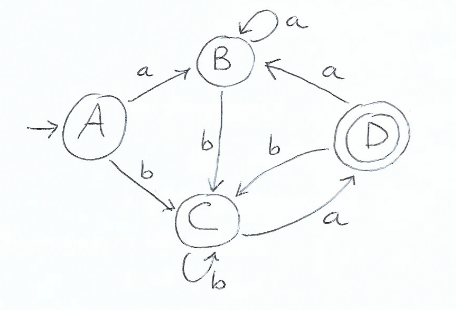
\includegraphics[width=0.4\textwidth]{img/DFA2.png}
\end{center} 
DFA ottenuto per costruzione per sottoinsiemi.
\subsection{$\epsilon$-closure e mosse}
Sia $q$ uno stato di un NFA. La $epsilon$-closure di $q$ è l'insieme degli stati raggiungibili da $q$ solo con mosse $\epsilon$.
\begin{align*}
\dfrac{}{\{q\} \subseteq epsilon\text{-closure}(q)} \quad \dfrac{p \in \epsilon\text{-closure}(q)}{\delta(p, \epsilon) \subseteq \epsilon\text{-closure}(q)}
\end{align*}
Sia $P$ un insieme di stati di un NFA 
\begin{align*}
\epsilon\text{-closure}(P) &= \bigcup_{p \in P} \epsilon\text{-closure}(p) \\
\text{mossa} &: \mathbb{P}(Q) \times \Sigma \to \mathbb{P}(Q) \\
\text{mossa} (P, a) &= \bigcup_{p \in P} \delta(p, a) \\
\triangle(A, b) &= \epsilon\text{-closure}(\text{mossa}(A, b))
\end{align*}
$\triangle(A, b)$ è la funzione di transizione del DFA.
\subsection{Algoritmo per calcolare la $\epsilon$-closure (P)}
Iniziallizzo $T = P$; \\
Inizializzo $\epsilon$-closure(P) P = P; \\
while $T \neq \emptyset$  do \{ \\
"scegli un $r \in T$ e rimuovilo da T" \\
for each $s \in \gamma(r, \epsilon)$ do \\
\quad if $s \notin \epsilon$-closure(P){     \\
\quad\quad add s to $\epsilon-$closure(P); \\
\quad\quad s to T;\}     \\
\} \\
\vspace{3em}
Usando la $\epsilon$-closure si può definire il linguaggio riconosciuto da un NFA in modo elegante
\begin{center}    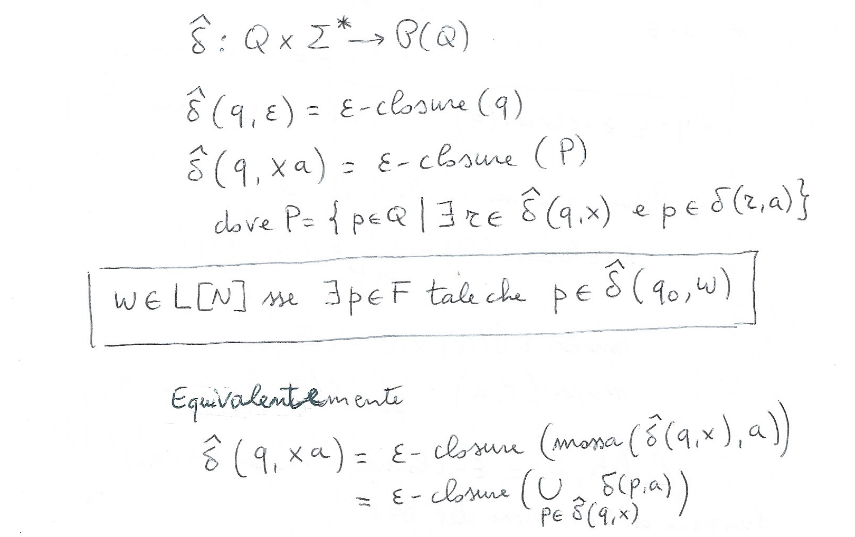
\includegraphics[width=0.5\textwidth]{img/elegante.png}
\end{center}
\subsection{Costruzione dei sottoinsimi}
Dato un NFA $N = \{\Sigma, Q, \delta, q_0, F \}$:
\begin{itemize}
  \item Inizializza $S = \epsilon$-closure($q_0$)
  \item Inizializza $T = \{ S\}$
  \item Finchè c'è un $ P \in T$ non marcato:
  \begin{itemize}
    \item $R = \epsilon$-closure(mossa(P,a));
    \item if $R \notin T$: add R to T;
    \item definisci $\triangle(P,a)=R$;
  \end{itemize}
\end{itemize}
Definiamo il DFA $M_N = \{\Sigma, T, \triangle, \epsilon\text{-closure}, \mathbb{F} \}$ dove $R \in \mathbb{F}$ sse $\exists q \in R$ con $q \in F$.
\begin{itemize}
  \item Nel caso pessimo $T = \mathbb{P}(Q)$ il DFA $M_N$ costituito a partire dall NFA N ha un numero di stati pari a $2^n$ dove $n = \mid Q \mid $
  \item Di solito $T$ è molto piu piccolo di $\mathbb{P}$(Q)
\end{itemize}
.
\begin{center}    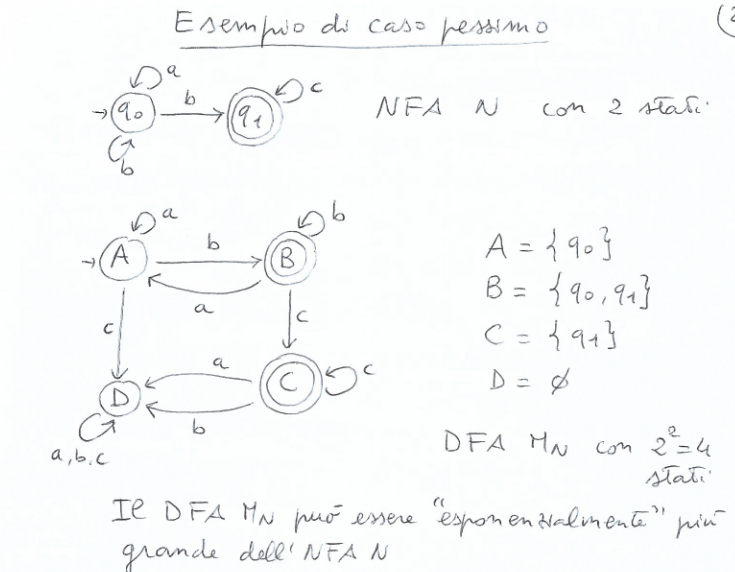
\includegraphics[width=0.5\textwidth]{img/pessimo.png}
\end{center}
\subsection{Equivalenza NFA-DFA}
Teorema: Sia $N = (\Sigma, Q, \delta, q_0, F)$ un NFA e sia $M_N$ l'automa ottenuto con la costruzione per sottoinsiemi. Allora $M_N$ è un DFA e si ha che
\begin{align*}
  L[N] = L[M]
\end{align*}
Corollario: La classe dei linguaggi riconosciuti dagli NFA coincide con la classe dei linguaggi riconosciuti dai DFA. \\
Dimostazione: mi rifiuto di scriverla (Lez06-Gorrieri.pdf slide 29-31).
\section{Da espressioni regolari a NFA equivalenti}
Teorema: Data una espressione regolare $s$, possiamo costruire un NFA $N[s]$ tale che $\mathbb{L}[S] = L[N[S]]$. Ovvero gli NFA riconoscono tutti i linguaggi regolari! \\
Dimostrazione: mi rifiuto di scriverla, pt. 2 (Lez07-Gorrieri.pdf slide 1-2). \\
\vspace{2em} \\
Esempio: \\
$S = (a \mid b)* ba$
\begin{center}    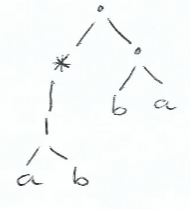
\includegraphics[width=0.2\textwidth]{img/albero1.png}
\end{center}
Partiamo dalle foglie e risaliamo alla radice (bottom-up)
\begin{center}    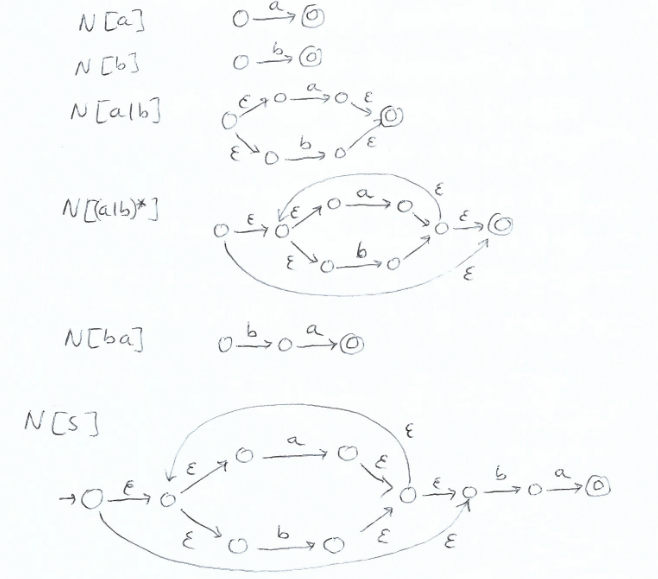
\includegraphics[width=0.6\textwidth]{img/es_albero1.png}
\end{center}
\subsection{Grammatiche regolari}
Def: Una grammatica libera è regolare sse ogni produzione è della forma $V \to aW$ oppure $V \to a$ dove $V, W \in NT$ e $a \in T$. Per il simbolo iniziale $S$  ammessa anche la produzione $S \to \epsilon$. \\
\vspace{2em} \\
Esempio:
\begin{align*}
  A \to aA \mid bB \mid bA \\
  B \to a
\end{align*}
$G$ è regolare, $L[G] = (a \mid b)^* ba$!! \\
\vspace{8em} \\
Proviamo ad associare una NFA a G:
\begin{center}    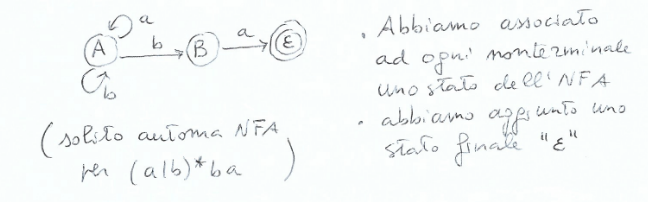
\includegraphics[width=0.6\textwidth]{img/proviamo.png}
\end{center}
\vspace{2em} 
Teorema: Data una grammatica regolare $G$ si può costruire un NFA $N_G$ equivalente.   \\
Dimostrazione: (Lez07-Gorrieri.pdf slide 6). \\
\vspace{3em} \\
Esempio: \\
\begin{center}    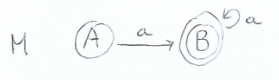
\includegraphics[width=0.2\textwidth]{img/esempio11.png}
\end{center}
$aa^*$ è l'espressione regolare che descrive $L[M]$. Secondo la costruzione appena descritta:     \\
\begin{center}    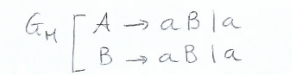
\includegraphics[width=0.3\textwidth]{img/teorema.png}
\end{center}
Secondo invece la variante     \\
  \begin{center}
    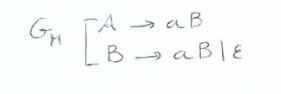
\includegraphics[width=0.3\textwidth]{img/variante.png}
\end{center}
a rigore questa non è regolare perchè ammette $B \to \epsilon$. \\
\subsection{Grammatiche regolari ed espressioni regolari}
Teorema: Il linguaggio definito da una grammatica regolare $G$ è un linguaggio regolare, cioè è possibile costruire una espressione regolare $S_G$ tale che 
\begin{align*}
  L(G) = \mathbb{L}[S_G]
\end{align*}
Dimostrazione: a pezzi (Lez07-Gorrieri.pdf slide 9-10) \\
\vspace{2em} \\
Esempio:
\begin{center}
    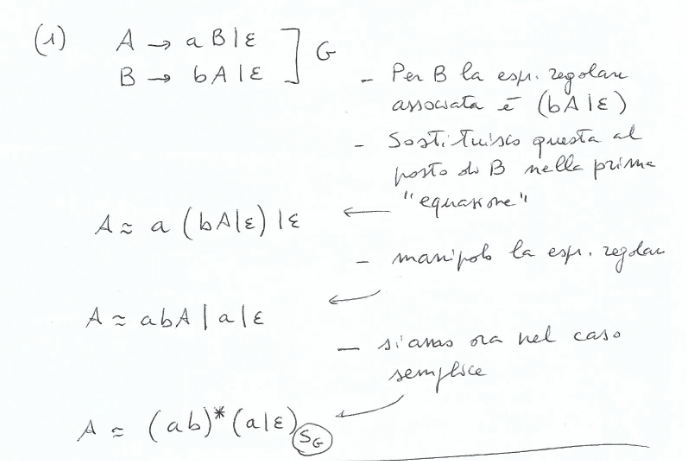
\includegraphics[width=0.6\textwidth]{img/esempio12.png}
\end{center}
Osservazione: La grammatica regolare con unica produzione $A \to aA ]G$ definisce il linguaggio vuoto, non $a^*$. Quindi $S_G = \emptyset$. \\
Riassumendo:
  \begin{center}
    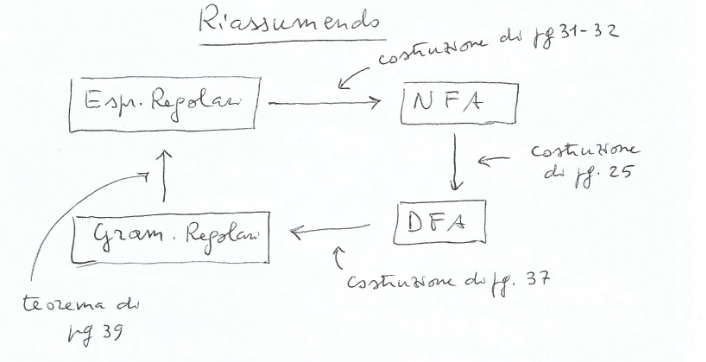
\includegraphics[width=0.6\textwidth]{img/riassumendo.png}
\end{center} 
Conseguenza: Tutti questi formalismi sono equivalenti! Tutti generano (grammatiche regolari) / riconoscono (NFA/DFA) / descrivono (espressione regolare) la stessa classe di linguaggio ovveri i linguaggi regolari. \\
Per costruire uno \textit{scanner} (analizzatore lessicale) si parte dalla specifica dei pattern associati alle categorie sintattiche del linguaggio, mediante espressioni regolari. \\
\begin{center}
  Espressioni regolari (pattern) $\to$ NFA $\to$ DFA 
\end{center}
Attenzione che se il NFA ha $n$ stati il DFA potrebbe avere $2^n$ stati! \\
Serve trovare un DFA equivalente più piccolo possibile 
\begin{center}
  min\_DFA $\quad$ (minimizzando)
\end{center}
\begin{itemize}
  \item per occupare meno memoria
  \item tale DFA minimo è unico (a meno di isomorfismo)
  \item ed è equivalente al DFA da cui siamo partiti
\end{itemize}
\section{Minimizzazione}
  \begin{center}
    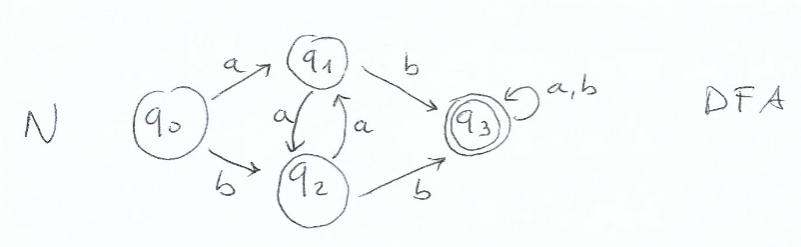
\includegraphics[width=0.6\textwidth]{img/minimizzazione.png}
\end{center} 
\begin{align*}
  L[N] = L[N, q_0] = (a \mid b)a^* b(a \mid b)^* \\
  L[N, q_1] = a^* b (a \mid b)^* = L[N, q_2]
\end{align*}
$\Rightarrow q_1$ e $q_2$ sono due stati equivalenti (o indistinguibili). \\
Se fondiamo un insieme $q_1$ e $q_2$, otteniamo un DFA più piccolo. 
  \begin{center}
    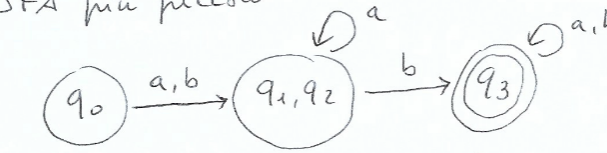
\includegraphics[width=0.6\textwidth]{img/piccolo.png}
\end{center} 
Questo DFA è \textit{minimo} perchè non ci sono due stati tra loro equivalenti. Infatti:
\begin{itemize}
  \item $q_3$ è \texttt{finale} e quindi $L[N, q_3] \ni \epsilon$
  \item $q_1, q_2$ è \texttt{non finale} e quindi $\epsilon \notin L[N, q, q_2]$ ma $b \in L[N, q, q_2]$
  \item $q_0$ è \texttt{non finale} ma $b \notin L[N, q_0]$
\end{itemize}
Prima delle definizione formali introduciamo questa notazione: 
\begin{center}
  Per un DFA $N = \{\Sigma, Q, \delta, q_0, F\}$ \\
  $\hat{\delta} : Q \to \Sigma* \to Q$ è definita come \\
  $\hat{\delta}(q, \epsilon)=q$ \\
  $\hat{\delta}(q, x a) = \delta(\hat{\delta}(q, x), a)$
\end{center}
e quindi 
\begin{align*}
  w \in L[N] \text{ sse } \hat{\delta}(q_0, w) \in F
\end{align*}
\vspace{3em} \\
\subsection{Equivalenza / Instinguibilità}
Definizione: Due stati $q_1$ e $q_2$ di un DFA $N$ sono equivalenti (o indistinguibili) se $\forall x \in \Sigma*$
\begin{align*}
  \hat{\sigma}(q_1, x) \in F \text{ sse } \hat{\delta}(q_2, x) \in F 
\end{align*}
\begin{center}
cioè se $L[N, q_1] = L[N, q_2]$
\end{center}
Simmetricamente due stati $q_1$ e $q_2$ non sono equivalenti se $\exists x \in \Sigma*$ tale che 
\begin{align*}
  \hat{\delta} (q_1, x) \in F \text{ ma } \hat{\delta}(q_2, x) \notin F 
\end{align*}
\begin{center}
o
\end{center}
\begin{align*}
  \hat{\delta} (q_1, x) \notin F \text{ ma } \hat{\delta}(q_2, x) \in F 
\end{align*}
$q_1$ e $q_2$ sono \texttt{distinguibili}! \\
\vspace{1em} \\
Strategia: cerco di distinguire due stati considerando le $x \in \Sigma*$ a partire della più corta ($\epsilon$).
  \begin{center}
    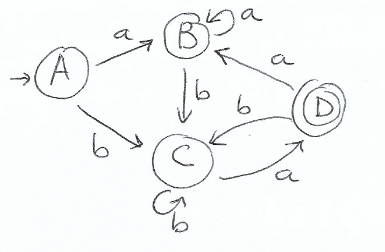
\includegraphics[width=0.3\textwidth]{img/capire.png}
\end{center} 
Cerco di vedere quali coppie di stati NON sono equivalenti, a cominciare dalla stringa $\epsilon$.
\begin{itemize}
  \item $\epsilon$ distingue ogni stati in $F$ da ogni stati in $Q \backslash F$ \\
  \begin{center}
  \tikz[baseline=(X.base)]{
  \node[inner sep=0] (X) {$(A,D)$};
  \draw (X.south west) -- (X.north east);
  } 
  \quad 
  \tikz[baseline=(X.base)]{
  \node[inner sep=0] (X) {$(B, D)$};
  \draw (X.south west) -- (X.north east);
  }
  \quad 
  \tikz[baseline=(X.base)]{
  \node[inner sep=0] (X) {$(C,D)$};
  \draw (X.south west) -- (X.north east);
  }
  \end{center}
  \item Consideriamo ora le stringhe di lunghezza 1, ovvero "a" e "b"
  \begin{itemize}
    \item \begin{itemize}
      \item "a" distingue $B$ e $C$ percheè $\delta(B, a) = B$ e $\delta(C, a) = D$ ma $(B,D)$ l'avevo giè cancellato al passo precedente ($B \in Q \backslash F$, mentre $D \in F$)! 
      \item "a" distingue $A$ e $C$ perchè $\delta(A, a) = B$ e $\delta(C,a)=D$ ma $B \in Q \backslash F$ mentre $D \in F$
    \end{itemize}
    \item "b" non mi permette di fare ulteriori distinzioni
  \end{itemize}
  \item Proceso ora con le stinghe lunghe 2, ma non riesco a fare nessuna ulteriore distinzione $\to$ FINE \\
  A e B sono equivalenti 
\end{itemize}
  \begin{center}
    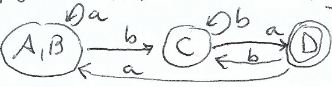
\includegraphics[width=0.3\textwidth]{img/equivalenti.png}
\end{center} 
\vspace{2em} 
Dato un DFA $M = (\Sigma, Q, \delta, q_0, F)$ definiamo una famiglia di relazioni $\sim_i \subseteq Q \times Q$ nel seguente modo:
\begin{itemize}
  \item $\sim_0 = \underbrace{F \times F \cup (Q \backslash F) \times (Q \backslash F)}_{\text{stati che non possono essere definiti da $\epsilon$, l'unica parola di lunghezza $o$}}$ \\
  \item $q_1 \sim_{i+1} q_2$ sse $\forall a \in \Sigma \quad \delta(q_1, a) \sim_i \delta(q_2, a)$ \\
  che significa: $q_1$ e $q_2$ sono in relazione $\sim_{i+1}$ se $\forall x \in \Sigma*$ con $\mid x \mid \leq i+1$ \\
  $\hat{\delta}(q_1, x) \in F$ sse $\hat{\delta}(q_2, x) \in F$ 
\end{itemize}
Osservazione:
\begin{itemize}
  \item La relazione $Id = \{(q,q) \mid q \in Q \}$ è tale che $Id \subseteq \sim_i$ per ogni $i$. \\
  "Uno stato è sempre equivalente a se stesso" 
  \item $\sim_i$ è una relazione d'equivalenza per ogni $i$
  \begin{itemize}
    \item $\sim_i$ ha 2 sole classi d'equivalenza, ovvero $F$ e $Q \backslash F$
    \item per $\sim_i$ riflessività e simmetria sono ovvie, mentre la transitivà è meno banale: \\
    $q_1 \sim_i q_2$ e $q_2 \sim_i q_2 \to q_1 \sim_i q_3$ 
  \end{itemize}
  \item $\sim_{i+1} \subseteq \sim_i$ \\
  "Ad ogni passo rimuovo qualche coppia" \\
  $\sim_o \supseteq \sim_1 \supseteq \sim_2 \supseteq \sim_3 \supseteq \dots$ \\
  catena descrescente di relazioni di equivalenza (non crescente)
  \item Se esiste un $k$ tale che $\sim_K = \sim_{K+1}$, allora $\forall f > k$ vale che $\sim_j = \sim_k$ \\
  "cioè non appena la relazione non viene modificata in un passo ho trovato la soluzione"
  \item Un tale $k$ esiste sicuramente ed è minore di \\
  \begin{align*}
    \mid \sim_0 \mid = \mid F \times F \mid + \mid (Q \backslash F) \times (Q \backslash F) \mid = {\mid F \mid}^2 + (Q \mid F)^2 
  \end{align*}
  perchè nella peggiore delle ipotesi ad ogni passo iterativo rimuovo solo una (meglio 2) coppia.
\end{itemize}
Ricorda: se $\sim_{k+1} = \sim_k$ allora $\forall j > k \quad \sim_j = \sim_k$ \\
Dimostrazione: (Lez08-Gorrieri.pdf slide 6) \\
\vspace{2em} \\
Vediamo ora
  \begin{center}
    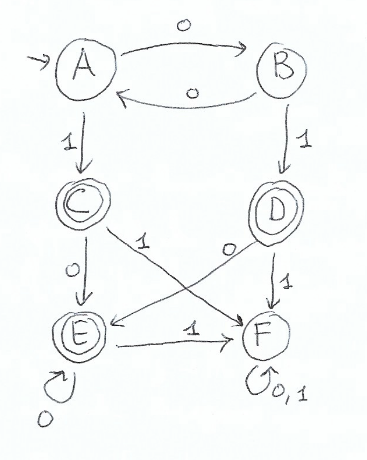
\includegraphics[width=0.3\textwidth]{img/esempio13.png}
\end{center} 
\begin{align*}
  \sim_0 = \{(A, A), (A,B),(A,F),\\
  (B,B),(B,A),(B,F),\\
  (F,F),(F,A),(F,B) \} \\ 
  \cup \{(C,C),(C,D),(C,E),\\
  (D,D),(D,C),(D,E),\\
  (E,E),(E,C),(E,D)\}
\end{align*}
\begin{align*}
  \sim_1 = \{(A, A), (A,B), \\
  (B,B),(B,A),\\
  (F,F),\\
  (C,C),(C,D),(C,E),\\
  (D,D),(D,C),(D,E),\\
  (E,E),(E,C),(E,D)\}
\end{align*}
\begin{align*}
\sim_2 = \sim_1 \text{ ok finito!}
\end{align*}
Quali stati sono equivalenti? Classi d'eq?
\begin{center}
- A e B $\quad$ - F $\quad$ -C,D,E
\end{center}
Automa minimo risultante della fusione degli stati equivalenti
  \begin{center}
    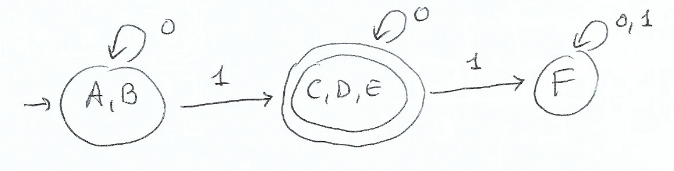
\includegraphics[width=0.5\textwidth]{img/esempio14.png}
\end{center} 
$L = 0^* 1 0^*$
  \begin{center}
    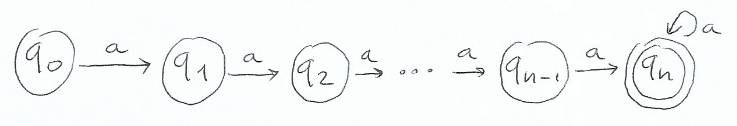
\includegraphics[width=0.5\textwidth]{img/esempio15.png}
\end{center} 
\begin{align*}
  \sim_0 = \{\{q_0, q_1, \dots, q_{n-1}\}, \{q_n\} \} \\
  \sim_1 = \{\{q_0, q_1, \dots, q_{n-2}\},\{q_{n-1}\}, \{q_n\} \} \\
  \vdots \\
  \sim_{n-1} = \{\{q_0\},\{q_1\},\{q_2\}, \dots, ,\{q_{n-1}\}, ,\{q_{n}\} \}
\end{align*}
\begin{center}
= Id identità \\
(ogni stato è equivalente solo a se stesso!)
\end{center}
\subsection*{Possiamo ricavare un algoritmo pratico da questa idea?}
\begin{itemize}
  \item Tabella con solo coppie "vere"
  \item al round 0 dell'algoritmo iterativo, metto una marca $x_0$ per segnare che la coppia è distinta (finale, nonfinale) (nonfinale, finale)
  \item al round 1, metto la marca $x_1$ per distinguere le coppie $(q_1, q_2)$ non ancora marcate per qualche $a \in \Sigma$ ha ($\delta(q_1, a), \delta(q_2, a)$) già marcata
  \item al round 2 metto la marca $x_2$ per $\dots$
\end{itemize}
Se non riesco a mettere nessuna nuova marcxa in un round $\to$ STOP!
  \begin{center}
    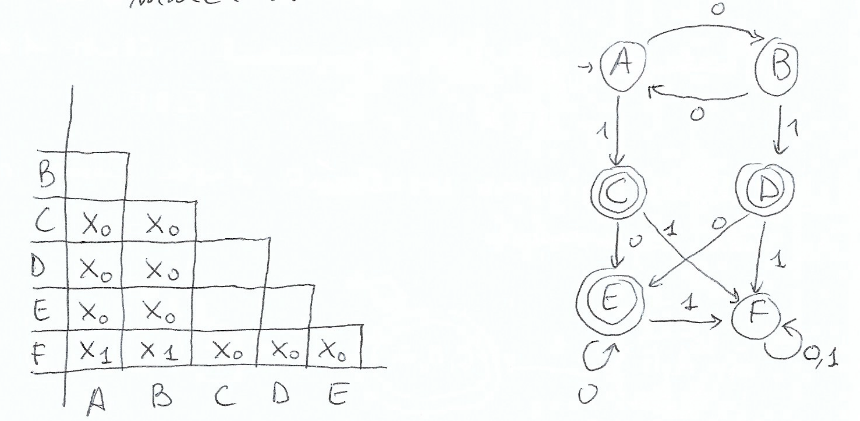
\includegraphics[width=0.5\textwidth]{img/esempio16.png}
\end{center} 
Le entrate della tabella che rimangono non marcate mi dicono quali stati sono equivalenti
\begin{center}
    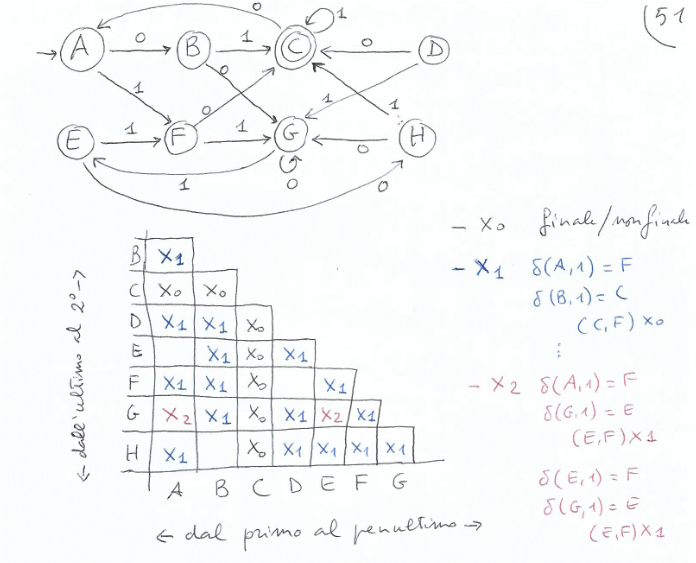
\includegraphics[width=0.7\textwidth]{img/esempio17.png}
\end{center} 
\begin{align*}
A \sim E \quad B \sim H \quad D \sim F
\end{align*}
  \begin{figure}
      \centering
    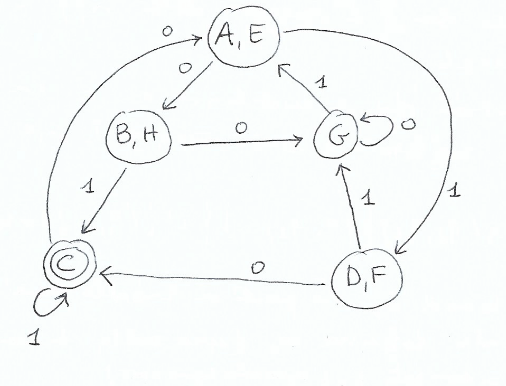
\includegraphics[width=0.5\textwidth]{img/esempio18.png}
    \caption{Automa minimo risultante}
    \label{fig:automa_minimo}
\end{figure}
\vspace{2em}
\subsection{Algoritmo iterativo (Tabella a scala)}
\begin{itemize}
  \item Costruire la tabella a scala
  \item Marca $x_0$ ad ogni coppia $(q_1, q_2)$ tale che $q_1 \in F$ e $q_2 \in Q \backslash F$ (o viceversa)
  \item $b \, := \, \text{ true }; \quad i \, := \, 1;$
  \item $\text{while } b \text{ do: }$ 
  \begin{itemize}
    \item $b \, := \, \text{ false } $
    \item per ogni coppia $(q_1, q_2)$ non marcata do:
    \begin{itemize}
      \item if $\exists a \in \Sigma$ con ($(q_1, a)$, $\delta(q_2, a)$) già marcata:
      \item then: \\
      - marca ($q_1, q_2$) con $x_i$ \\
      - $b \, := \, \text{true}$
    \end{itemize}
    \item $i \, := \, i + 1$
  \end{itemize}
  \item Al termine sia $J$ l'insieme delle coppie non marcate
  \item La relazione di equivalenza $\sim$ è la chiusura riflessiva e simmetria di $J$ cioè
  \begin{align*}
    \sim = J \cup \{(q_2, q_1) \mid (q_1, q_2) \in J \} \cup \{(q,q) \mid q \in Q \}
  \end{align*}
\end{itemize}
Nota: al round $i$ la parte di tabella non marcate definisce $\sim_i$ (una volta chiusa riflessivamente e simmetricamente)
\vspace{2em} \\
Teorema: Dato un DFA $M=(\Sigma, Q, \delta, q_0, F)$ l'algoritmo di riempimento della tabella a scala termina. Due stati $p$ e $q$ sono distinguibili (ovvero non equivalenti) sse la casella ($p, q$) ($\sigma(q,p)$) è marcata (e quindi sono equivalenti sse la casella non è marcata)\\
Dimostrazione: (Lez08-Gorrieri.pdf slide 12) \\
Vediamo ora un esempio:
\begin{center}
    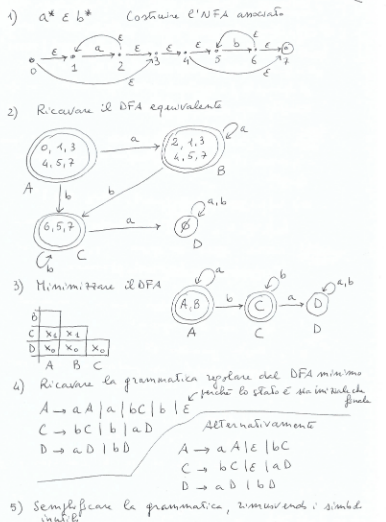
\includegraphics[width=0.7\textwidth]{img/esempio19.png}
\end{center} 
\begin{center}
    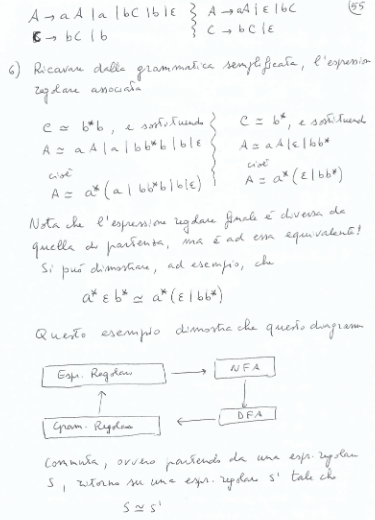
\includegraphics[width=0.7\textwidth]{img/esempio20.png}
\end{center} 
\subsection{Automa minimo}
Dato un DFA $M=\{\Sigma, Q, \delta, q_0, F\}$ l'automa minimo equivalente $M_{min} = (\Sigma, Q_{min}, \delta_{min}, [q_0], F_{min})$ è dato da:
\begin{itemize}
  \item $Q_{min} = \{[q] \mid q \in Q \}$ con $[q] = \{q' \in Q \mid q \sim q' \}$ \\
  (gli stati di $M_{min}$ sono classi di equivalenza di stati di $M$)
  \item $\delta_{min}([q], a) = [\delta(q, a)]$ 
  \item $F_{min} = \{[q] \mid q \in F\}$
\end{itemize}
Osservazione: Non esistono 2 stati distinti in $M_{min}$ che siano tra loro equivalenti: $[q] \neq [q'] \to q \sim q'$
\vspace{10px} \\
\textbf{Notazioni: } \\
\vspace{5px} \\
\begin{minipage}{0.45\textwidth}
    DFA $M$
    \begin{align*}
      \hat{\delta} \, : \, Q \times \Sigma* \to Q \\
      \hat{\delta}(q, \epsilon) = q \\
      \hat{\delta}(q, xa) = \delta(\hat{\delta}(q,x),a)\\
      w \in L[M] \text{ sse } \hat{\delta}(q_0, w) \in F
    \end{align*}
\end{minipage}%
\hfill
\begin{minipage}{0.45\textwidth}
    DFA $M_{min}$
    \begin{align*}
    \hat{\delta}_{min} \, : \, Q_{min} \times \Sigma* \to Q_{min} \\
    \hat{\delta}_{min}([q], \epsilon) = [q] \\
    \hat{\delta}_{min}([q], xa) = \hat{\delta}_{min}(\hat{\delta}_{min}([q], x), a) \\
    w \in L[M_{min}] \text{ sse } \hat{\delta}_{min}([q_0], w) \in F_{min}
     \end{align*}
\end{minipage} \\
\vspace{2em} \\
Teorema: Dato un DFA $M=(\Sigma, Q, \delta, q_0, F)$ l'automa $M_{min} = (\Sigma, Q_{min}, \delta_{min}, [q_0], F_{min})$ riconosce lo stesso linguaggio di $M$, ed ha il minimo numero di stati tra tutti gli automi deterministici per questo linguaggio. \\
Dimostrazione: (Lez08-Gorrieri.pdf slide 17-19) \\
\vspace{2em} \\
\section{Lex: Generatore di Scanner}
\begin{itemize}
  \item Un Lex è un software che gira sotto Unix scritto nel 1995. 
  \item Flex è un free software scritto nel 1987
  \item \texttt{Lex / Flex} è un generatore di analizzatore lessicale.
    \begin{itemize}
      \item Input: un file "\textit{.l}" che contiene un insieme di definizioni regolare ed una serie di azioni corrispondenti
      \item Output: un programma C che realizza l'automa riconoscitore e che associa ad ogni istanza di una definiziona la relativa azione \\
\end{itemize}
 \begin{minipage}{0.25\textwidth}
        Sorgente Lex per il linguaggio $\mathbb{L}$ \\(\texttt{lex.l}) 
     \end{minipage}
     $\to$
     \begin{minipage}{0.15\textwidth}
        \boxed{\text{Lex compilar}}
     \end{minipage}
    $\to$ 
     \begin{minipage}{0.40\textwidth}
    Analizzatore lessicale per $\mathbb{L}$ \\(programma C di nome \texttt{lex.yy.c})
     \end{minipage} \\
     \vspace{2em} \\
    $\to$ 
    \begin{minipage}{0.20\textwidth}
        \boxed{\text{Compilatore C}} 
    \end{minipage}
    $\to$ 
    \begin{minipage}{0.20\textwidth}
      \texttt{a.out} \\(eseguibile)
    \end{minipage} \\
    \end{itemize}
\subsection{Come è fatto un file di input \textit{lex.l}?}
Diviso in 3 parti
\begin{itemize}
    \item Dichiarazioni (definizioni regolari) \\
    Esempi: \\
    cifre [0-9] \\
    ide [a-zA-Z]([a-zA-Z] | [0-9]$)^*$
    \item Regole: $\underbrace{\text{\{espressione regolare\}}}_{\text{pattern}}$ $\underbrace{\text{\{azione\}}}_{\text{frammento del codice C}}$ \\
    Esempi: \\
    \{cifre\} \, \{printf("<num, \%s>", yytext); \} con \texttt{yytext} come variabile che contiene il testo matched!
    \item Funzioni ausiliarie (se si usano funzioni complesse nalla parte "azione" questo sono definite qua)
\end{itemize}
\subsection*{Come funziona il programma \texttt{lex.yy.c}?}
Il programma C ottenuto, e compilato per renderlo eseguibile in \texttt{a.out}, implementa essenzialmente il DFA riconoscitore dell'insieme delle espressioni regolari contenute nelle "regole".
\begin{itemize}
  \item scandisce il testo sorgente alla ricerca di una stringa che corrisponda (cioè sia un lessemma per) una delle espressioni regolari. (pattern di categoria sintattica) 
  \item quando riconosce un lessemma, esegue l'azione specificata, e passi in output il risultato dell'azione al posto del lessemma
  \item quando l'input non corrisponde a nessun pattern, lo lascia inalterato e "segnala" la cosa al "gestore degli errori"
\end{itemize}
Esempio banale
\begin{center}
    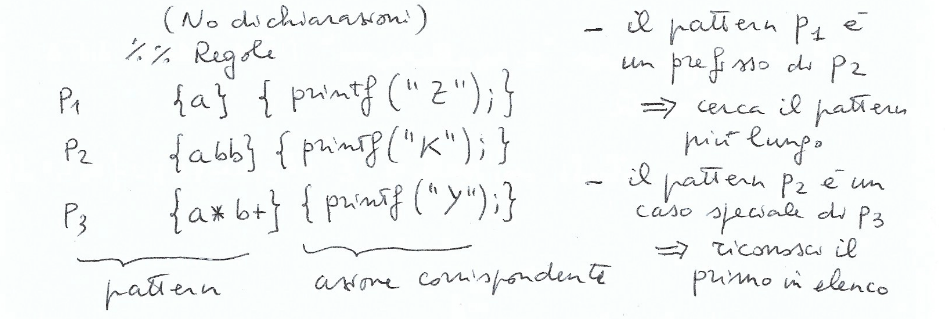
\includegraphics[width=0.6\textwidth]{img/esempio21.png}
\end{center} 
\begin{center}
    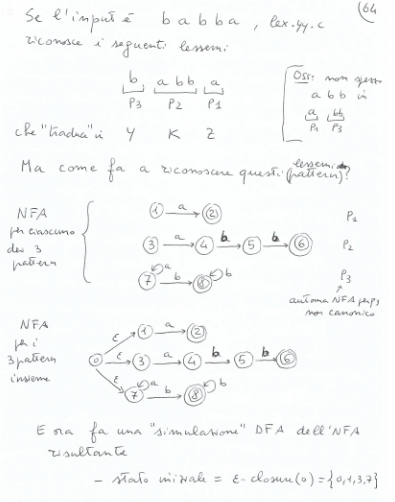
\includegraphics[width=0.6\textwidth]{img/esempio22.png}
\end{center} 
\vspace{5em} 
\begin{center}
    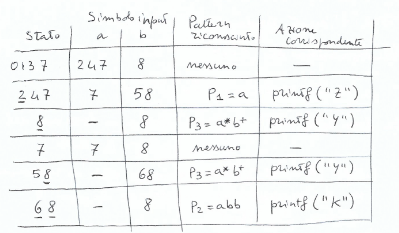
\includegraphics[width=0.8\textwidth]{img/esempio23.png}
\end{center}  
\vspace{5em} 
\texttt{a.out} procede in questo modo:
\begin{itemize}
  \item va avanti a leggere l'input finchè non si blocca
  \item se lo stati in cui si trova è di riconoscimento $\to$ OK. Altrimenti torna indietro fino a trovare uno stato di riconoscimento (ovver se 2 sttai pososno essere riconosciuto si sceglie il più lungo) 
  \item se arrivati al "match" vediamo che potenzialmente più di un pattern andrebbe bene allora prendiamo quello elencato prima 
\end{itemize}
Vediamo il funzionamento sull'input
\begin{center}
  babba
\end{center}
Inizio in 
\begin{center}
  0137 $\to^b$ f $\not\to^a$
\end{center}
Mi sono bloccato in $f \to b$, è un lessemma dal pattern $P_3 = a^* b^+$. \\
Ora l'input residuo è "abba". \\
Ricominciamo da 0137
\begin{center}
  0137 $\to^a$ 247 $\to^b$ 58 $\to^b$ 68 $\not\to^a$
\end{center}
Mi sono bloccato in $68 \to $ "abb" è un lessemma del pattern $P_2 = abb$. \\
Ricominciamo da 0137 col residuo a
\begin{center}
  0137 $\to^a$ 247 
\end{center}
FINE $\to$ a è un lessemma dal pattern $P_1 = a$. \\
\vspace{2em}
Nel file \texttt{.l} di un linguaggio di programmazione le parole riservate vanno messe prima degli identificatori
\begin{center}
  while $\quad$ Az1 \\
  if $\quad$ Az2 \\
  $\vdots$ \\
  ide $\quad$ AzIDE
\end{center}
Se trovo "while" riconosco subito la parola riservata prima, se trovo "whiles" va in IDE perchè prendo il match più lungo. \\
\vspace{1em} \\
Vediamo un esempio di un analizzatore lessicale in Lex.
\begin{center}
    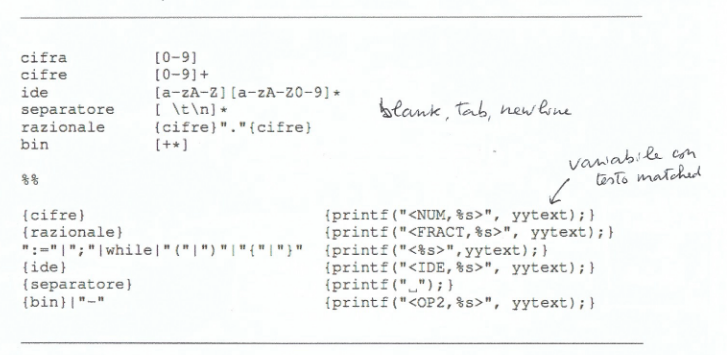
\includegraphics[width=0.8\textwidth]{img/esempio24.png}
\end{center}  
\subsection{Utilizzo con YACC}
\begin{center}
    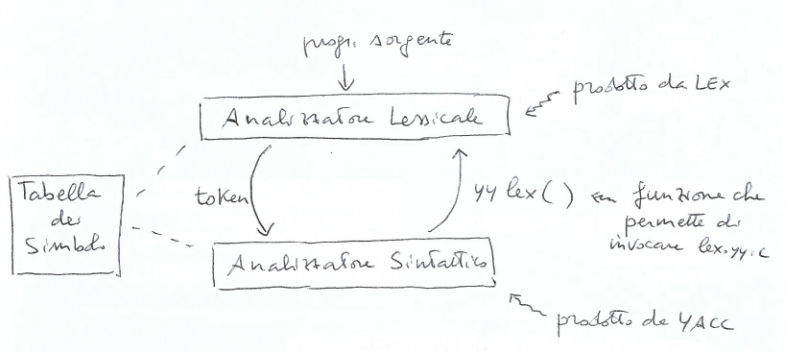
\includegraphics[width=0.8\textwidth]{img/yacc.png}
\end{center}  
\begin{itemize}
  \item il programma generato da LEX non è usato da solo
  \item è una subroutine per YACC (generatore di analizzatore sintattico)
  \item alcune variabili comuni ai due programm permettono di scambiarsi informazioni
  \item \texttt{lex.yy.c} è usato da YACC "on-demand" richiedendolo il tolken successivo
  \item \texttt{yylex())} restituisce il nome del token, mentre il valore del token è condiviso nella variabile \texttt{yyeval}
\end{itemize}
\begin{center} 
    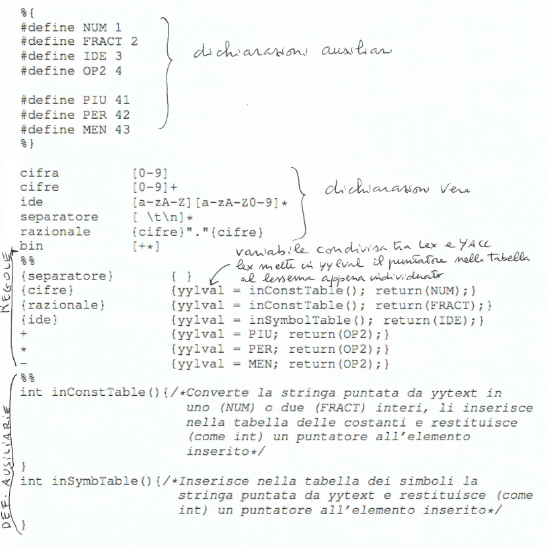
\includegraphics[width=0.8\textwidth]{img/esempio25.png}
\end{center}  
\subsection{Proprietà algoritmiche dei linguaggi regolari}
Finora non abbiamo dimostrato che esistono linguaggi non regolari. Sappiamo che una grammatica regolare è un caso speciale di grammatica libera. Quindi sicuramente
\begin{align*}
  \text{Linguaggi liberi} \subseteq \text{Linguaggi regolari}
\end{align*}
Ora vedremo una proprietà algoritmica dei linguaggi regolari che sarà utile per dimostare che certi linguaggi, non pessedendo quelle proprietà, non sono regolari! \\
Vediamo per esempio
\begin{align*}
L = \{a^n b^n \mid n \geq 0 \} \quad \text{ è sicuramente libero}
\end{align*}
perchè generato da una grammatica libera $S \to \epsilon \mid aSb$ e dimostreremo che non è regolare! \\
\vspace{1em} \\
Intuitivamente perchè $\{a^n b^n \mid n \geq 0 \}$ non può essere regolare?
\begin{center}
Necessita di contare illimitatamente e per farlo mi servirebbero infiniti stati
\end{center}
\begin{center}
    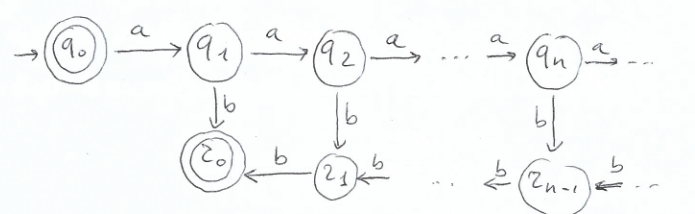
\includegraphics[width=0.5\textwidth]{img/esempio26.png}
\end{center} 
Se devo farlo $\forall n \geq 0$ mi servono infiniti stati! Un NFA / DFA ha solo un numero finito di stati, per cui può solo "contare" tanto quanto gli stati che ha.
\subsection{Pumping Lemma}
Se $L$ è linguaggio regolare allora $\exists N > 0$ tale che $\forall z \in L$ con $\mid Z \mid \geq N$, $\exists u,v,w$ tale che
\begin{itemize}
  \item $z = uvw$
  \item $\mid uv \mid \leq N$
  \item $\mid v \mid \geq 1$
  \item $\forall k \geq 0 \quad uv^k w \in L$
\end{itemize}
Inoltre $N$ è minore o uguale del numero di stati del DFA minimo che accetta L.\\
Dimostrazione: (Lez09-Gorrieri.pdf 12-13) \\
\vspace{2em} \\
Come usare il pumping lemma per dimostrare che un linguaggio non è regolare? 
\begin{center}
  Se $L$ è regolare $\to P$ \\
  Se $\sim P \to$ L non è regolare
\end{center}
\subsection*{Negazione del pumping lemma}
\begin{align*}
\text{Se }
[ \forall N > 0 \quad \exists z \in L \text{ con } \mid z \mid \geq N \\
\forall uvw \text{ se } \\
1.\,  z = uvw \\
2. \mid uv \mid \leq N \\
3. \mid v \mid \geq 1  \\
\text{allora $\exists k \geq 0$. $uv^k w \notin L]$ }
\end{align*}
allora $L$ non è regolare. \\
\vspace{2em} \\
Dimostriamo che $L = \{a^n b^n \mid n \geq 1 \}$ non è regolare.
\begin{center}
    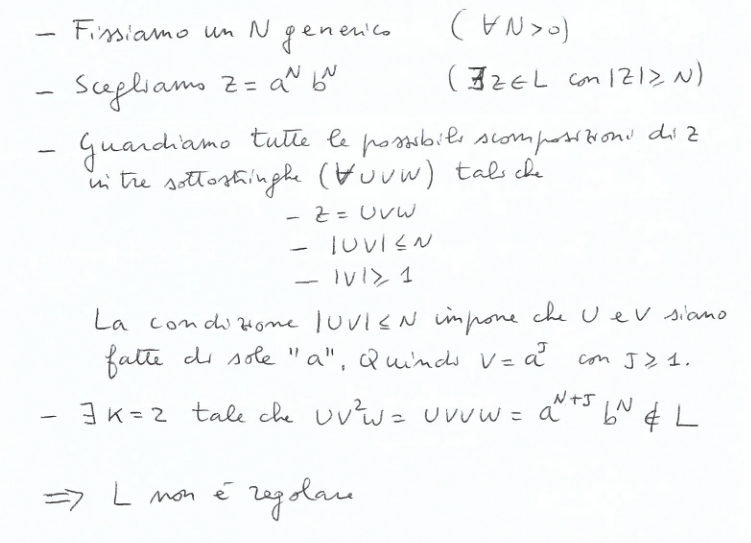
\includegraphics[width=0.8\textwidth]{img/esempio27.png}
\end{center}
\subsection*{Altre proprietà dei linguaggi regolari}
La classe dei linguaggi regolari è chiusa per
\begin{itemize}
  \item unione
  \item concatenazione
  \item stella di Kleene
  \item complementazione
  \item intersezione
\end{itemize}
Dimostrazione: (Lez09-Gorrieri.pdf slide 19-21) \\
\vspace{2em} \\
\section{Analisi sintattica: linguaggi liberi}
\begin{itemize}
  \item classi di linguaggi più generale di quella dei linguaggi regolari 
  \begin{center}
    Linguaggi liberi $\subseteq$ Linguaggi regolari
  \end{center} 
  \item grammatiche libere da contesto più generale di quelle regolari \\
  \begin{minipage}{0.45\textwidth}
   Regolari: \\
   $V \to aW$ \\
   $V \to a \quad V, W \in NT$ \\
   $S \to \epsilon \quad a \in T$
  \end{minipage}
  \begin{minipage}{0.45\textwidth}
  Libere: \\
  $V \to \zeta \quad \zeta \in (T \cup NT)^*$
  \end{minipage} \\
  \item automi a pila (pushdown automata - PDA) invece di automi finiti (NFA - DFA) \\
\end{itemize}  
\subsection{Analisi sintattica}
\begin{center}
    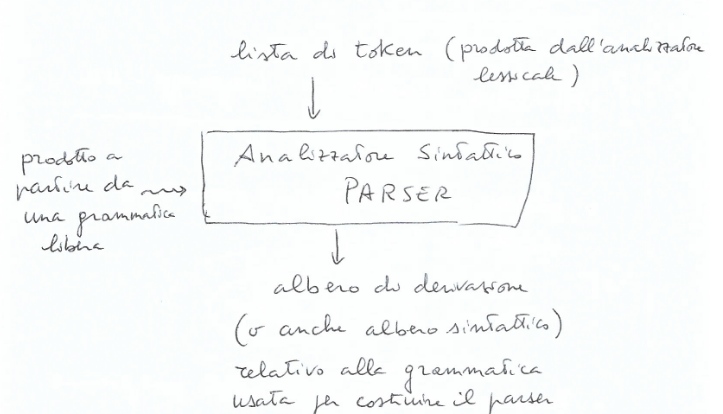
\includegraphics[width=0.7\textwidth]{img/analisi_sintattica.png}
\end{center} 
Come bisogna potenziare gli NFA / DFA per far si che riconoscano linguaggi liberi? \\
Esempio $L = \{ww^R \mid w \in \{a,b\}^* \}$
\begin{itemize}
  \item L è libero perchè $L = L(G)$ con $G[S \to \epsilon \mid aSa \mid bSb]$ libera
  \item L non è regolare 
  \item $L = \{\epsilon, aa, bb, aaaa, abba, baab, bbbb, \dots \}$
\end{itemize}  
L'automa deve "ricordare" la prima metà dell'input (cioè w) in modo da confrontarla con la seconda metà (cioè $w^R$) in ordine inverso. Questo porta di accumulare (parte) dell'input, e quindi fornire all'utoma memoria ausiliaria; una pila che può crescere illimitatamente. \\
\vspace{1em} \\
Quando si accorge che $w$ è finita? In genere non c'è un criterio, l'automa assume di essere arrivato a metò e inizia a confrontare con l'indietro.
\begin{center}
    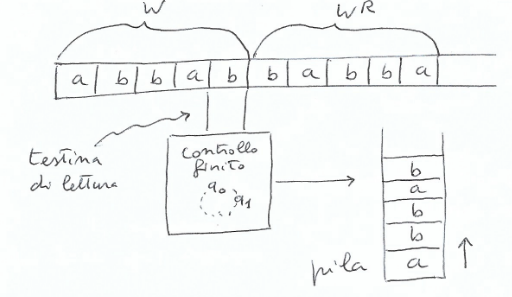
\includegraphics[width=0.5\textwidth]{img/indietro.png}
\end{center} 
La pila può crescere senza limiti, ma può leggere solo l'elemento top della pila. Può rimuovere solo l'elemento top, e può inserire solo in testa. \\
\vspace{2em} \\
Definizione: Un automa a pila non deterministico (PDA) è una 7-pla $(\Sigma, Q, \Gamma, \delta, q_0, \bot, F)$ dove
\begin{itemize}
  \item $\Sigma$ è un alfabeto finito (simboli in input)
  \item $Q$ è un insieme finito di stati
  \item $\Gamma$ è un insieme finito di simboli della pila
  \item $\delta$ è la funzione di transizione con tipo
  \begin{align*}
    \delta : Q \times (\Sigma \cup \{\epsilon\}) \times \Gamma \to \mathbb{P}_\text{fin} (Q \times \Gamma^*)
  \end{align*}
  \item $q_0$ è lo stato iniziale 
  \item $\bot \in \Gamma$ è il simbolo iniziale sulla pila
  \item $F \subseteq Q$ è l'insieme degli stati finali
\end{itemize}
\begin{align*}
\delta : Q \times 
(\underbrace{\Sigma \cup \{\epsilon\}}_{\parbox{5cm}{consuma un simbolo del input ($\Sigma$ oppure no ($\epsilon$))}}) 
\underbrace{\times \Gamma}_{\text{consuma il simbolo top della pila}}
\to \mathbb{P}_\text{fin} (\underbrace{Q \times \Gamma^*}_{\parbox{5cm}{sulla pila scrive una stringa di lunghezza qualsiasi (anche $\epsilon$) di simboli in $\Gamma$}}) 
\end{align*}
è nondeterministico perchè
\begin{itemize}
  \item $\mid \delta(q, \sigma, A) \mid$ può essere > 1
  \item ma se anche richiedessimo che $\mid \delta(q', \sigma, B) \mid \leq 1$ potrebbero esistere $\mid \delta(q', \epsilon, B) \mid = 1$ e $\mid \delta(q', b, B) \mid = 1$ $\to$ nondeterminismo tra mossa $\epsilon$ e mossa "b".
\end{itemize}
\vspace{2em} 
\subsection*{Transizione di un PDA}
\begin{itemize}
  \item descrizione istantanea (q, w, b)
  \begin{itemize}
    \item $q \in Q$ (stato corrente) 
    \item $w \in \Sigma^*$ (input ancora non letto)
    \item $b \in \Gamma^*$ (stringa sulla pila)
  \end{itemize}
  \item mossa
  \begin{align*}
    \dfrac{(q', \zeta) \in \delta(q, a, X)}{(q, aw, xB) \rotatebox{90}{$\top$}_N (q', w, \zeta B)} \quad a \in \Sigma
  \end{align*}
    \begin{align*}
    \dfrac{(q', \zeta) \in \delta(q, \epsilon, X)}{(q, w, xB) \rotatebox{90}{$\top$}_N (q', w, \zeta B)} 
  \end{align*}
  \item computazionale / cammino
  \begin{align*}
    \dfrac{}{(q,w,B) \rotatebox{90}{$\top$}_N (q, w, B)} \quad \dfrac{(q,w,B) \rotatebox{90}{$\top$}_N^* (q',w',B')\rotatebox{90}{$\top$}_N(q'',w'',B'')}{(q,w,B)\rotatebox{90}{$\top$}_N^* (q'',w'',B'')}
  \end{align*} \\
  (Chiusura riflessiva e transivita di $\rotatebox{90}{$\top$}_N$)
\end{itemize}
\subsection{Linguaggio accettato}
Due modalità di riconoscimento:
\begin{itemize}
  \item Per stato finale 
  \[
    \{ w \in \Sigma^* \mid (q_0, w, \bot)
    \rotatebox{90}{$\top$}_N^* (q, \epsilon, \zeta)
    \text{ con } q \in F \}
  \]
  \item Per pila vuota
  \[
    P[N] = \{ w \in \Sigma^* \mid (q_0, w, \bot)
    \rotatebox{90}{$\top$}_N^* (q, \epsilon, \epsilon) \}
  \]
\end{itemize}
con $N = \{\Sigma, Q, \Gamma, \delta, q_0, \bot, F\}$. \\
Nota: spesso per un PDF $L[N] \neq P[N]$, però se $L=L[N]$ allora esiste un $N'$ tale che $L=P[N']$ e viceversa.
\vspace{1em} \\
Esempio: $\{ww^R \mid w \in \{a,b\}^*\}$\\
$N = (\Sigma, Q, \Gamma, \delta, q_0, \bot, F)$ dove
\begin{align*}
  \Sigma = \{a,b\} \\
  \Gamma = \{a,b,\bot\} \\
  Q = \{s_0, s_1, s_2 \} \\
  q_0 = s_0 \\
  F = \{s_2\}
\end{align*}
\begin{align*}
  \delta(s_0, a, x) = \{(s_0, ax)\} \quad \forall x \in \Gamma \\
  \delta(s_0, b, x) = \{(s_0, bx)\} \quad \forall x \in \Gamma \\
  \delta(s_0, \epsilon, x) = \{(s_1, x)\} \quad \forall x \in \Gamma \\
  \delta(s_1, a, a) = \{(s_1, \epsilon)\} \\ 
  \delta(s_1, b, b) = \{(s_1, \epsilon)\} \\ 
  \delta(s_1, \epsilon, \bot) = \{(s_2, \epsilon)\} \\ 
  \delta(s_2, \zeta, x) = \emptyset \quad \forall \zeta \in \Sigma \cup \{ \epsilon \}, \quad \forall x \in \Gamma
\end{align*}
\begin{figure}
  \centering
  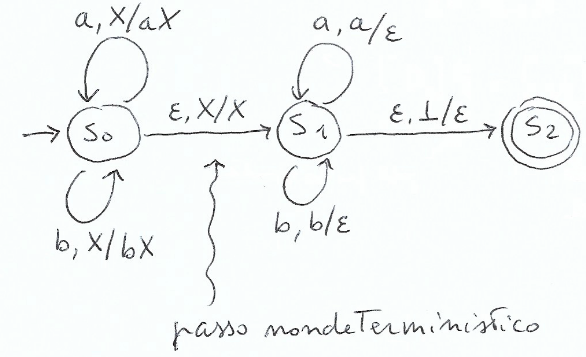
\includegraphics[width=0.5\textwidth]{img/transizione2.png}
  \caption{Diagramma di transizione}
  \label{fig:transizione2}
\end{figure}
\begin{center}
    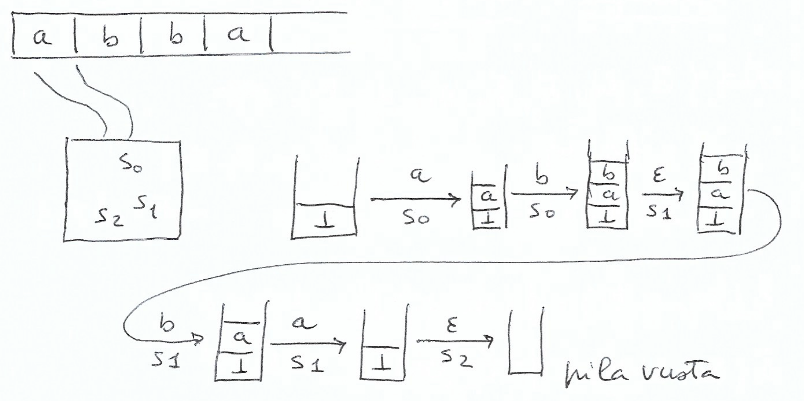
\includegraphics[width=0.5\textwidth]{img/transizione3.png}
\end{center} 
\begin{itemize}
  \item esiste una "computazione" per \textit{abba} che porta l'automa $N$ allo stato finale $s_2$ (così come svuotare la pila)
  \item si può vedere che "svuota la pila" sse vado allo stato $s_2$
  \begin{align*}
    \to \underbrace{L[N]}_{\text{per stato finale}} = \underbrace{P[N]}_{\text{per pila vuota}}
  \end{align*}
\end{itemize}
\vspace{1em} 
Esempio: PDA $L = \{wcw^R \mid w \in \{a,b\}^* \}$
\begin{center}
    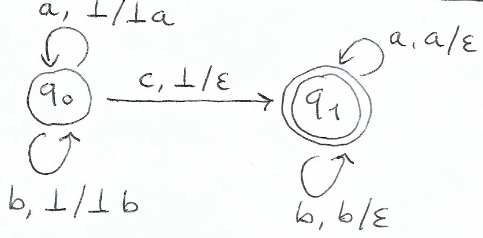
\includegraphics[width=0.5\textwidth]{img/esempio28.png}
\end{center} 
\begin{itemize}
  \item N è deterministico:
  \begin{itemize}
    \item $\mid \delta(q, a, z) \mid \leq 1 \quad \forall q \in Q, \forall a \in \Sigma \cup \{\epsilon\}, \quad \forall z \in \Gamma$
    \item se $\delta(q, \epsilon, z) \neq 0$, allora $\delta(q, a, z) = \emptyset \quad \forall a \in \Sigma$
  \end{itemize}
  \item $L = P[N]$ cioè il linguaggio $L$ è riconosciuto per la pila vuota
  \item $L[N] = \{wcy \mid w \in \{a,b\}^* \text{ e } y \text{ è prefisso di } w^R\}$
  \item se l'input è \textit{acab} questo non viene letto tutto, $N$ si blocca dopo aver letto \textit{aca} sullo statp finale cioè rinosce \textit{aca} ma non \textit{acab}
\end{itemize}
\begin{align*}
  L = \{wcw^R \mid w \in \{a,b\}^* \}
\end{align*}
\begin{center}
    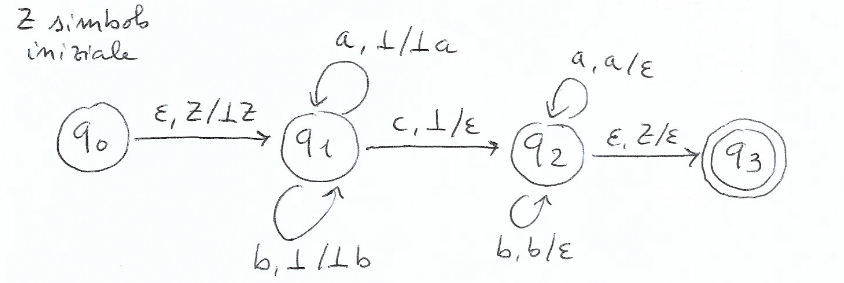
\includegraphics[width=0.5\textwidth]{img/esempio29.png}
\end{center} 
$L = L[N] = P[N]$. \\
$N$ è deterministico e riconosce $L$ sia per stato finale sia per pila vuota. \\
\vspace{2em} \\
La classe dei linguaggi rinosciuti per pila vuota o per stato finale non cambia.\\
\textbf{Teorema}:
\begin{itemize}
  \item Se $L = \underbrace{P[N]}_{\text{per pila vuota}}$ possiamo costruire $N'$ tale che $L = L[N']$
  \item Se $L = \underbrace{L[N]}_{\text{per stato finale}}$ possiamo costruire $N'$ tale che $L = P[N']$
\end{itemize}
Dimostrazione: (Lez10-Gorrieri.pdf slide 13) \\
\vspace{2em} \\
Al contrario come ottenere un PDA a partire da una grammatica libera? Un possibile metodo (top-down) è il seguente 
\begin{align*}
  S \to aSb \mid \epsilon
\end{align*}
\begin{center}
    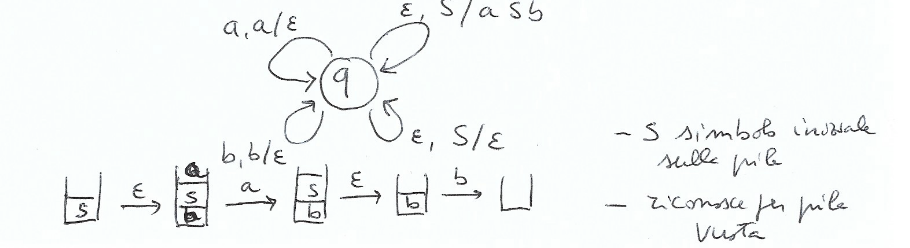
\includegraphics[width=0.7\textwidth]{img/contrario.png}
\end{center} 
\begin{align*}
  A \to aAa \mid bAb \mid \epsilon
\end{align*}
PDA con un solo stato con $A$ sulla pila come simbolo iniziale che riconosce per pila vuota.
\begin{center}
    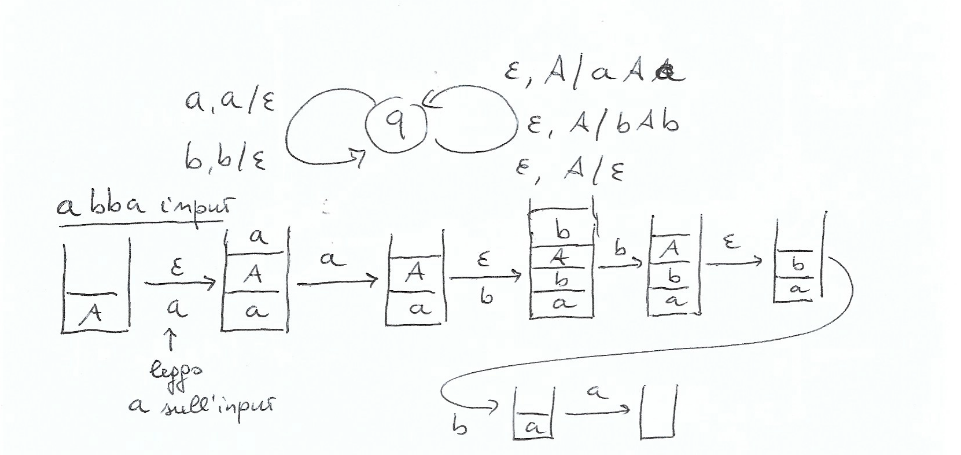
\includegraphics[width=0.5\textwidth]{img/vuota.png}
\end{center} 
Costruire una derivazione \textit{leftmost} a partire da $A$
\begin{align*}
  A \to aAa \to abAba \to abba
\end{align*}
\begin{center}
    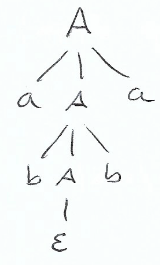
\includegraphics[width=0.2\textwidth]{img/albero2.png}
\end{center} 
\vspace{2em} 
\textbf{Teorema}: Un linguaggio $L$ è libero da contesto se è accettato da un PDA. \\
Dimostrazione: (Lez10-Gorrieri.pdf slide 17-18). \\
\vspace{2em} \\
Ricapitolando: un linguaggio $L$ è libero sse è accettato da un PDA (nondeterministico).
\vspace{2em} \\
\section{Proprietà di chiusura}
Teorema: I linguaggi liberi sono chiusi per
\begin{itemize}
  \item unione
  \item concatenazione
  \item ripetizione (stella di Kleene)
\end{itemize}
Dimostrazione: (Lez11-Gorrieri.pdf slide 1) \\
\vspace{2em} \\
Teorema: L'intersezione $L_1 \cap L_2$ di un linguaggio libero $L_1$ con un linguaggio regolare $L_2$ e' un linguaggio libero. \\
Dimostazione: (Lez11-Gorrieri.pdf slide 2) \\
\vspace{1em}\\
Esercizio: 
\begin{center}
  Mostrare che $L_1 \cap L_2$ con
\end{center}
\begin{align*}
  L_1 = \{a^nb^n \mid n \geq 0\} \text{ e } L_2 = \{w \in \{a,b\}^* \mid \exists k \in \mathbb{N}, \, \mid w \mid = 4k\}
\end{align*}
\begin{center}
  e' un linguaggio regolare.
\end{center}
\begin{itemize}
  \item Applicando il teorema si ha che $L_1 \cap L_2$ e' livero perche' $L_1$ e' libero ($S \to aSb \mid \epsilon$) e $L_2$ e' regolare
  \begin{center}
    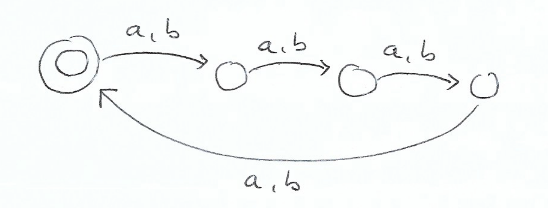
\includegraphics[width=0.5\textwidth]{img/esempio30.png}
  \end{center}
  \item $L_1 \cap L_2 = \{a^{2n}b^{2n} \mid n \geq 0\}$ ed e' libero perche' $S \to aaSbb \mid \epsilon$ lo genera.
\end{itemize}
\vspace{1em} 
\subsection{Applicazione del teorema}
$L = \{ww \mid w\in\{a,b\}^*\}$ e' libero? Se lo fosse allora anche $L \, \cap \,  a^* b^* a^* b^* = \{a^n b^m a^n b^m \mid n,m \geq 0 \}$ dovrebbe esserlo. Ma dimostreremo presto che questo linguaggio non e' libero.
\begin{center}
  $\to$ nemmeno $L$ puo' essere libero
\end{center}
\textit{Osservazione}: Vale che
\begin{itemize}
  \item Se $L_1 \cap L_2$ e' non regolare, ma $L_2$ e' regolare allora $L_1$ non e' regolare. (chiuso per intersezione)
  \item Se $L_1 \cap L_2$ e' non libero, ma $L_2$ e' regolare allora $L_1$  non libero. (interesezione di un libero e un regolare da un libero)
\end{itemize}
\vspace{1em} 
\textbf{I linguaggi libero non sono chiusi per interesezione}
\begin{center}
  $L_1 = \{a^n b^n c^m \mid n,m \geq 0\}$ e' libero \\
  $L_2 = \{a^n b^m c^m \mid n,m \geq 0\}$ e' libero \\
  $L_1 \cap L_2 = \{a^n b^n c^n \mid n \geq 0\}$ e' non libero!
\end{center}
\vspace{1em}
\textbf{I linguaggi liberi non sono chiusi per complementazione}
\begin{align*}
  L_1 \cap L_2 = \overline{\overline{L_1} \cap \overline{L_2}}
\end{align*}
Cioe' se fossero chiusi per complementazione allora dovrebberlo esserlo anche per intersezione.
\begin{center}
   $\to$ non sono chiusi per complementazione
\end{center}
\subsection{Pumping Theorem}
Se $L$ e' libero allora $\exists N > 0$ tale che $\forall z \in L$ con $\mid z \mid \geq N, \, \exists u,v,w, x, y$ tale che
\begin{itemize}
  \item $z = uvwxy$
  \item $\mid vwx \mid \leq N$
  \item $\mid vx \mid \geq 1$
  \item $\forall k \geq 0 \quad uv^kwx^ky \in L$
\end{itemize}
Dimostrazione: Sia $G = (\text{NT, T, R, S})$ una grammatica libera tale che $L = L(G)$.
\begin{itemize}
  \item Sia $b$ il massimo fattore di ramificazione in un albero di derivazione (ovvero il massimo numero di simboli che compaiono nella parte destra di una produzione in R)
  \begin{align*}
    b = \text{max}\{\mid \zeta \mid \, \mid \, A \to \zeta \in \text{R}\}
  \end{align*}
  Osservazione: $b \geq 2$, altrimenti la gramamtica sarebbe banale
  \item Un albero di altezza $h$ (con $o$ la radice) e fattore di ramificazione $b$ ha al piu' $b^h$ foglie
    \begin{center}
    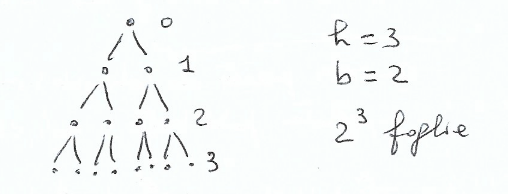
\includegraphics[width=0.5\textwidth]{img/esempio31.png}
  \end{center}
\end{itemize}
Fissiamo $N = b^{\mid NT \mid +1}$ (quindi $N > b^{\mid NT \mid}$ dato che $b \geq 2$). \\
Allora ogni albero di derivazione per $z$, con $\mid z \mid \geq N$ deve avere altezza almeno $\mid NT \mid +1$. \\
Prendiamo un qualunque $z \in L$, con $\mid z \mid \geq N$. Consideriamo il suo albero di derivazione (se ne possiede piu' di uno perche' $G$ e' ambigua, prendiamo quello con il minor numero di nodi). Dunque:
\begin{align*}
  \mid z \mid \geq N \to \text{ albero con alteza $\geq \mid NT \mid +1$} \\
  \to \exists \text{ un cammino da radice $S$ ad una foglia con almeno $\mid NT \mid +2$ nodi} 
\end{align*}
\begin{align*}
    \to \text{ Quel cammino attraversa $\mid NT \mid +1$ nodi interni etichettati con un nonterminale (la foglie e' etichettata da un terminale)} 
\end{align*}
\begin{align*}
    \to \text{ almeno un nonterminale si ripete in quel cammino}
\end{align*}
Allora $S \to^* z$ puo' essere diviso come
\begin{align*}
  S \to^* \underbrace{uAy \to^* uvAxy}_{\text{questa parte di derivazione può essere ripetuta più volte}} \to^* uvwxy
\end{align*}
Esempio: $S \to^* uAy \to^* uvAxy \to^* uv^2Ax^2y \to^* uv^2wx^2y$
\begin{center}
    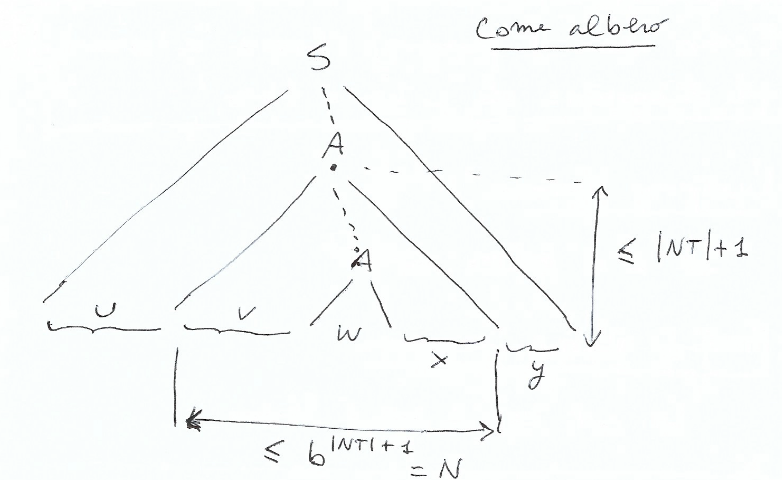
\includegraphics[width=0.5\textwidth]{img/esempio32.png}
\end{center}
Allora
\begin{itemize}
  \item $S \to^* uAy \to^* uwy \quad k=0$
  \item $S \to^* uAy \to^* uvAxy \to^* uvwxy \quad k=1$
  \item $S \to^* uAy \to^* uvAxy \to^* uv^2Ax^2y \quad k=2$
  \item $\vdots$
\end{itemize}
Bisogna solo verificare i vincoli:
\begin{itemize}
  \item $\mid vx \mid \geq 1$
  \begin{itemize}
    \item Ovvio: se entrambe $\epsilon$ allora l'albero per $k=0$ generebbe ancora $z$ ed avrebbe meno nodi contraddicendo l'ipotesi di aver scelto il piu' piccolo albero
  \end{itemize}    
  \item $\mid vwx \mid \leq N$
  \begin{itemize}
    \item Ovvio: il cammino da $A$ alla foglia di lunghezza $\leq \mid NT \mid +1$ (cioe' usa $\mid NT \mid +2$ nodi al massimo di cui uno e' il terminale foglia) $\to$ la $A$ in alto non puo' generare parola piu' lunghe di $b^{\mid NT \mid +1} = N$
  \end{itemize}
\end{itemize}
\vspace{2em}
\subsection*{Come usare il pumping theorem "a rovescio" per dimostrare che $L$ non e' libero?}
\textbf{Pumping Theorem}
\begin{center}
  Se $L$ e' libero $\to P$
\end{center}
\textbf{Pumping Theorem a rovescio}
\begin{center}
  Se $\sim P \to L$ non e' libero
\end{center}
\vspace{1em}
Se $\forall N > 0 \quad \exists z \in L $ con $\mid z \mid \geq N$ tale che 
\begin{align*}
  \forall u,v,w,x,y
\end{align*}
\begin{itemize}
  \item $z = uvwzy$
  \item $\mid vwx \mid \leq N$
  \item $\mid vx \mid \geq 1$
\end{itemize}
allora $\exists k \leq 0$. $uv^kwx^ky \notin L$. \\
Allora $L$ non e' libero.
\vspace{2em} \\
Dimostriamo che certi linguaggi non sono liberi perche' soddisfano la proprieta' $\sim P$.
\begin{align*}
  L = \{a^n b^n c^n \mid n \geq 0\} \text{ e' libero? NO!}
\end{align*}
\begin{itemize}
  \item Fissiamo $N > 0$ generico ($\forall N > 0$)
  \item Scegliamo $z = a^nb^nc^n$ ($\exists z \in L, \text{ con } \mid z \mid \geq N$)
  \item Per ogni $u,v,w,x,y$ tale che
  \begin{itemize}
    \item $z = uvwxy$
    \item $\mid vwx \mid \leq N$
    \item $\mid vx \mid \geq 1$
  \end{itemize}
\end{itemize}
\begin{align*}
  \to \text{ le 2 estremita' di $vwx$ non possono essere "a" e "c"}
\end{align*}
\begin{itemize}
  \item caso $vwx$ non contiene $c$ (ovvero tutti i $c$ stanno in $y$) \\
  $\quad \to uv^2wx^2$ cambia il numero di $a$ e/o $b$ ma non quelle di $c$.  ($uv^2wx^2y \notin L$)
  \item caso $vwx$ non contiene $a$ (le "a" stanno tutte in $U$) \\
  $\quad \to uv^2wx^2y \notin L$
\end{itemize}
$\to L$ non e' libero!
\vspace{2em} \\
\subsection{Classificazione di Chomsky}
\begin{itemize}
  \item Grammatiche regolari
  \begin{align*}
    A \to aB \\
    A \to a \\
    S \to \epsilon
  \end{align*}
  \item Grammatiche libere da contesto 
  \begin{align*}
    A \to \zeta \text{ con } \zeta \in (NT \cup T)^+ \\
    S \to \epsilon
  \end{align*}
  \item Grammatiche dipendenti dal contesto
  \begin{align*}
    yA\delta \to yw\delta \\
    y, \delta \in (NT \cup T)^* \\
    w \in (NT \cup T)^+ \\
    S \to \epsilon
  \end{align*}
  \item Grammatiche monotone
  \begin{align*}
    y \to \delta \text{ con } \mid y \mid \leq \mid \delta \mid
  \end{align*}
  \item Grammatiche generali (a strutttura di frase)
  \begin{align*}
    y \to \delta \text{ (senza alcun vincolo)}
  \end{align*}
\end{itemize}
\begin{center}
    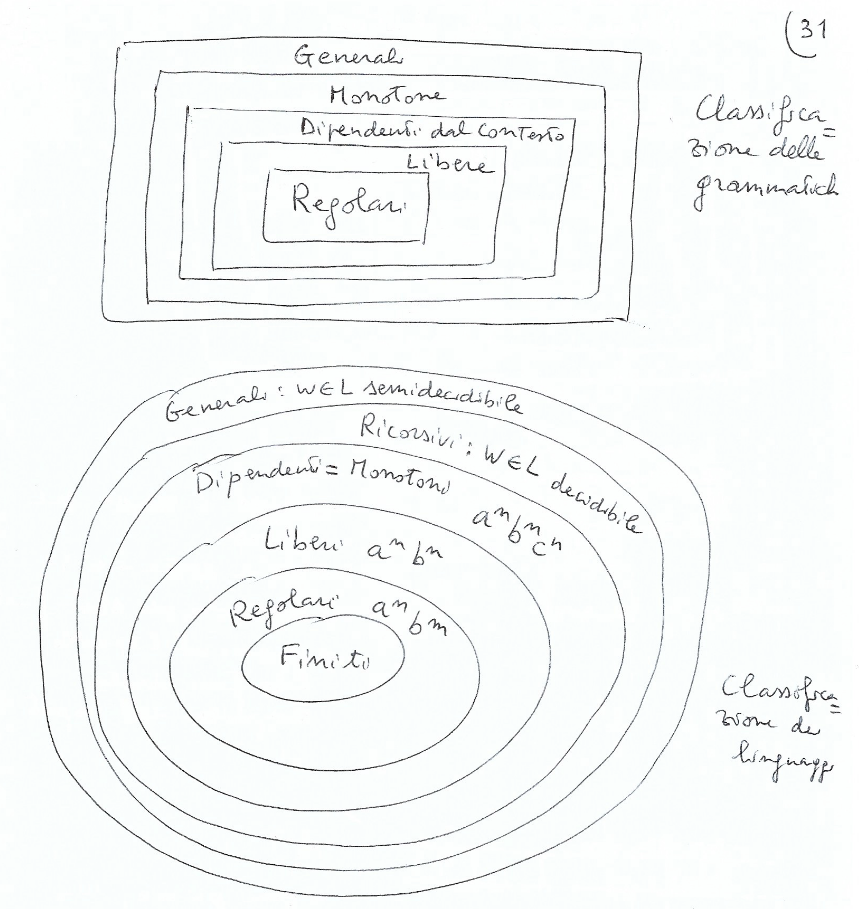
\includegraphics[width=0.7\textwidth]{img/esempio33.png}
\end{center}
\begin{center}
    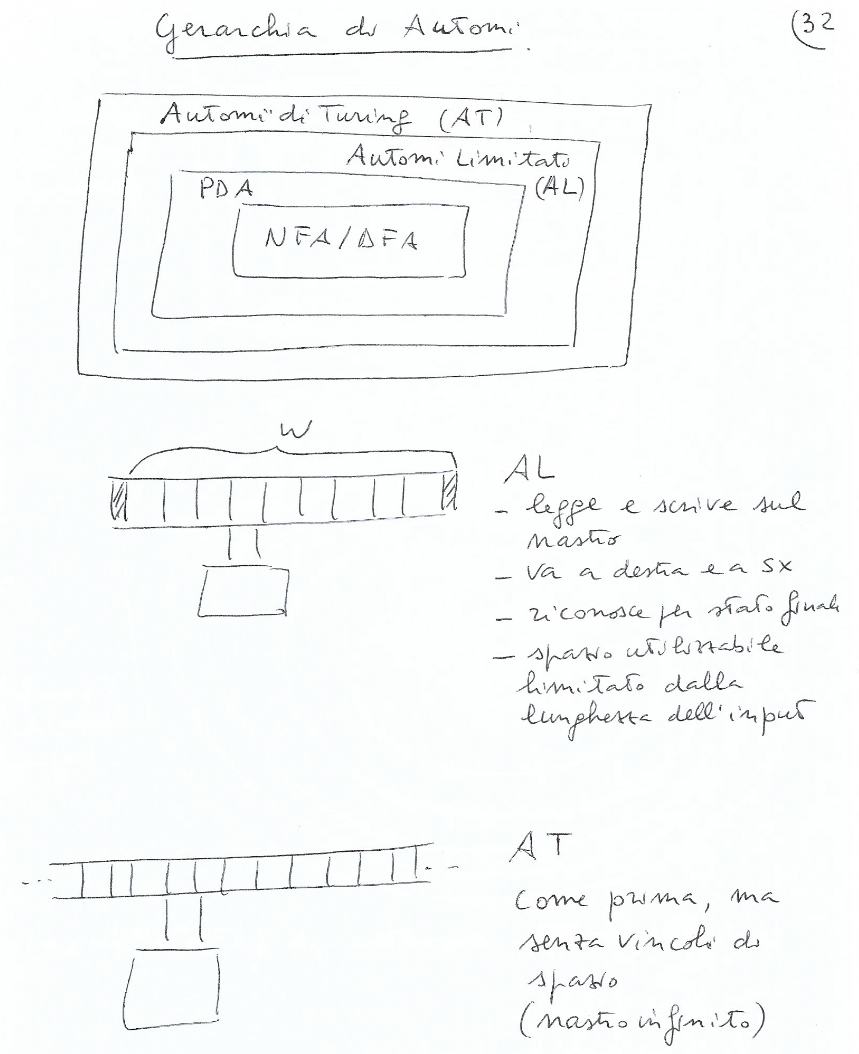
\includegraphics[width=0.9\textwidth]{img/esempio34.png}
\end{center}
\section{PDA e linguaggi deterministici}
Definizione: Un PDA $N = \{\Sigma, Q, \Gamma, \delta, q_0, \bot, F\}$ e' \texttt{deterministico} (DPDA) sse
\begin{itemize}
  \item $\forall q \in Q \, \forall z \in \Gamma$ se $\delta(q, \epsilon, z) \neq \emptyset$ allora $\delta(q, a, z) = \emptyset \quad \forall a \in \Sigma$
  \item $\forall q \in Q \quad \forall z \in \Gamma \quad \forall a \in \Sigma \cup \{\epsilon\} \, \mid \delta(q, a,z) \mid \leq 1$
\end{itemize}
Definizione: Un linguaggio e' libero deterministico se e' accettato per stato finale da un DPDA. \\
Teorema: La classe dei linguaggi liberi deterministici e' inclusa propriamente nella classe dei linguaggi liberi. \\
\vspace{1em} \\
Proposizione: Se $L$ e' regolare allora $\exists $ DPDA $N$ tale che $L = \underbrace{L[N]}_\text{per stato finale}$.
\vspace{1em}\\
Dimostrazione: Se $L$ e' regolare allora $\exists $ DFA $M$ tale che $L = L[M]$. A partire da $M$ posso costriure un DPDA $N$ che si comporta come $M$ senza mai manipolare lo stack
\begin{align*}
  \to L = L[N]
\end{align*}
\begin{center}
    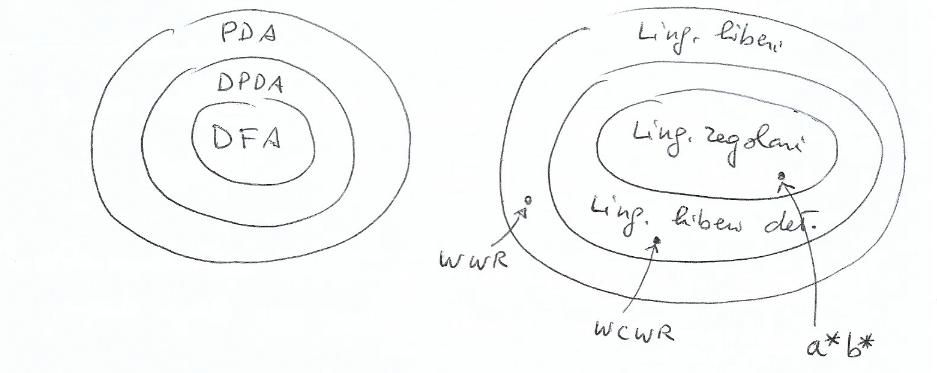
\includegraphics[width=0.7\textwidth]{img/esempio35.png}
\end{center}
Fatto: Un linguaggio libero deterministico $L$ e' riconosciuto da un DPDA per pila vuota se sse $L$ gode della \textit{rpefix propriety}.
\begin{align*}
  \boxed{\exists x,y \in L \text{ tale che } x \text{ e' prefisso di } y}
\end{align*}
Osserva che $L_2 = \{wcw^R \mid w \in \{a,b\}^*\}$ gode della prefix propriety.
\begin{center}
    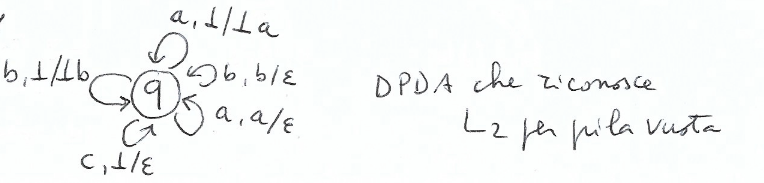
\includegraphics[width=0.7\textwidth]{img/esempio36.png}
\end{center}
Quindi
\begin{itemize}
  \item Se $L$ libero non determinanistico non gode della prefix propriety non puo' essere riconosciuto da un DPDA per pila vuota.
  \item Se $L$ e' libero deterministico gode della prefix propriety allora puo' essere riconosciuto da un DPDA per prila vuota
  \item Se $L$ e' libero deterministico allora $L \mathdollar = \{w \mathdollar \mid w \in L\}$ gode della prefix propriety \\
  $\quad \to L \mathdollar$ puo' essere riconosciuto da un DPDA per pila vuota
\end{itemize} 
\vspace{1em}
Proposizione: Se $L$ e' libero determinisico (cioe' riconosciuto da un DPDA per stato finale) allora $L$ e' generabile da una gramamtica libera NON AMBIGUA.
\begin{center}
  $\to$ I linguaggi liberi deterministici non sono ambigui!!
\end{center}
\subsection{Proprieta' dei linguaggi liberi deterministici}
\begin{itemize}
  \item Sono chiusti per complementazione cioe' se $\exists $ DPDA $N$ tale che $L = L[N]$ allora esiste un DPDA $N'$ tale che $\overline{L} = \Sigma^* \backslash L$ \\
  \vspace{1em} \\
  Idea della prova: Bisogna rendere totale la $\delta$ di $N$, eventualmente aggiungendo degli stati non finali e poi $N'$ si ottiene da questo $N$ aumento, semplicemente scambiando finali e nonfinali (come fatto con DFA per dimostare che i regolari sono chiusi per complementazione)
  \item Non sono chiusi per interesezione 
  \begin{align*}
    L_1 = \{a^n b^n c^m \mid n,m \geq 0\} \text{ e' libero deterministico} \\
    L_2 = \{a^m b^n c^n \mid n,m \geq 0\} \text{e' libero deterministico} \\
  \end{align*} \\
  ma 
  \begin{align*}
    L_1 \cap L_2 = \{a^n b^n c^n \mid n \geq 0\} \text{ non e' libero!}
  \end{align*}
  \item Non sono chiusi per unione \\
  \begin{itemize}
    \item Se per assurdo lo fossero allora
    \begin{align*}
      L_1 \cap L_2 = \overline{\overline{L_1} \cup \overline{L_2}}
    \end{align*}
    e quindi risulterebbero chiusi per interesezione. $\to$ impossibile!
  \end{itemize}
\end{itemize}
\subsection{Analizzatori sintattici (Parser)}
\begin{center}
    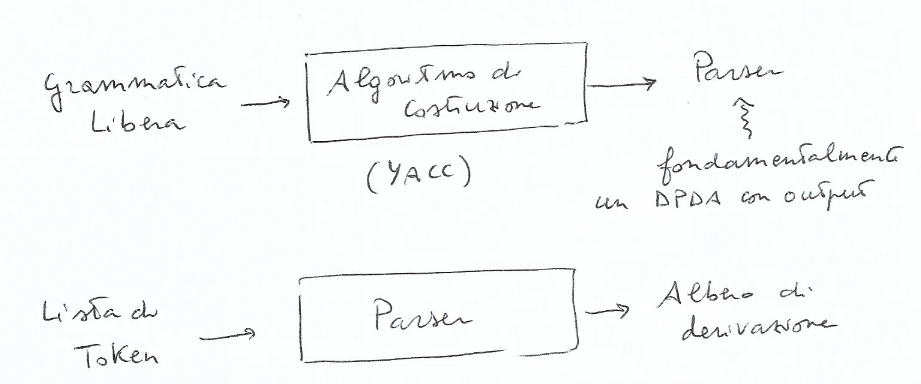
\includegraphics[width=0.7\textwidth]{img/parser.png}
\end{center}
I parser possono essere
\begin{itemize}
  \item Nondeterministici: se durante la ricerca di una derivazione si scopre che una scelta e' improduttiva e non porta a riconoscere l'input il parser torna indietro (backtracking), disfa parte della derivazione appena costruita e sceglie un'altra produzione tornando a leggere (parte del)l'input
  \item Deterministici: leggono l'input una sola volta, ogni loro decisione e' definitiva
\end{itemize}
Entrambi cercano di sfruttare informazioni dall'input per guidare la ricerca della derivazione. \\
\vspace{2em} \\
I parser possono essere:
\begin{itemize}
  \item \textbf{Top-down}:
  \begin{itemize}
    \item Ricostruiscono una derivazione \textit{leftmost} per $w$ a partire dal simbolo iniziale $S$ (all'inizio sulla pila)
  \end{itemize}
  \item Bottom-up:
  \begin{itemize}
    \item Ricostruiscono una derivazione \textit{rigthmost} (a rovescio) a partire dalla stringa $w$ cercando di ridurla al simbolo iniziale $S$ (alla fine sulla pila)
  \end{itemize}
\end{itemize}
Entrambi cercano di sfruttura quello che vedono dell'input per guidare la ricerca di derivazione
\subsection*{Introduzione al top-down parsing}
Data $G = \{NT, T, S, R\}$ libera, costruiamo il PDA $M = (T, \{q\}, T \cup NT, \delta, q, S, \emptyset)$ che riconosce per pila vuota dove $\delta$ e' definita:
\begin{itemize}
  \item $(q, \beta) \in \delta(q, \epsilon, A)$ se $A \to \beta \in R$ (espandi) 
  \item $(q, \epsilon) \in \delta(q, a, a) \quad \forall a \in T$ (consuma)
\end{itemize}
tale che $L[G] = \underbrace{P[M]}_\text{riconoscimento per pila vuota}$
\begin{itemize}
  \item Nondeterminismo! Puo' essere risolto scegliendo la produzione in base al simbolo in lettura (look-head!)
  \begin{itemize}
    \item se leggo "a" $\to$ espando $S \to aSb$
    \item se leggo "b" $\to$ espando $S \to \epsilon$
  \end{itemize}
  \begin{center}
    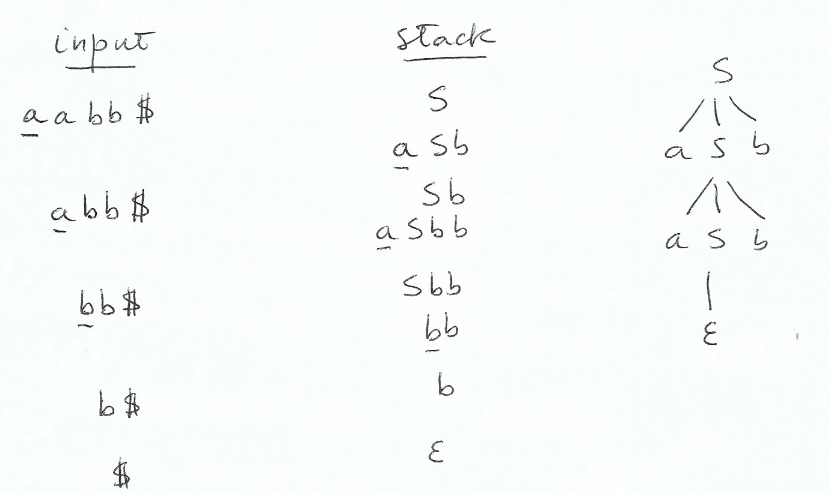
\includegraphics[width=0.7\textwidth]{img/esempio37.png}
\end{center}
\end{itemize}
\begin{align*}
  G[ S \to aSb \mid \epsilon
\end{align*}
Vedremo essere una grammatica di classe $LL(1)$ nel senso che consente di costruire un Parser / DPDA
\begin{align*}
  \underbrace{\text{left-to-rigth}}_\text{modo in cui viene letto l'input} / \underbrace{\text{left-derivation}}_\text{genera una derivazione \textit{leftmost}} \underbrace{\text{(1)}}_\text{guardando un solo simbolo di look-head}
\end{align*}
\vspace{1em}\\
\begin{align*}
  G[ S \to aSb \mid ab
\end{align*}
In questo caso devo guardare 2 simboli di look-head
\begin{itemize}
  \item se leggo "aa" $\to$ espando $S \to aSb$ 
  \item se leggo "bb" $\to$ espando $S \to ab$
\end{itemize}
$G$ e' di classe $LL(2)$
\vspace{1em} \\
\subsection*{Introduzione al bottom-up parsing}
Data una grammatica libera $G = (NT, T, R, S)$ costruiamo un PDA $M$ che rinosce $L(G)\cdot \mathdollar$
\begin{align*}
  M = (T, \{q\}, T \cup NT \cup \{a\}, \delta, q, z, \emptyset)
\end{align*}
dove
\begin{itemize}
  \item $(q, ax) \in \delta(q,a,x) \quad \forall a \in T, \quad \forall x \in T \cup NT \cup \{a\}$ (SHIFT)
  \item $(q, A) \in \delta(q, \epsilon, \underbrace{\zeta^R}_{\parbox{7cm}{\centering
generalizzazione dei PDA\\
in cui si consuma una stringa sulla pila\\
anziché solo il top}})$ se $A \to \zeta \in R$ (REDUCE)
  \item $(q, \epsilon) \in \delta(q, \underbrace{\mathdollar}_\text{simbolo di fine input}, \underbrace{Sz}_\text{$S$ deve essere alla fina sulla pila})$ (ACCEPT)
\end{itemize}
Esempio: 
\begin{align*}
  G[ S \to aSb \mid ab
\end{align*}
  \begin{center}
    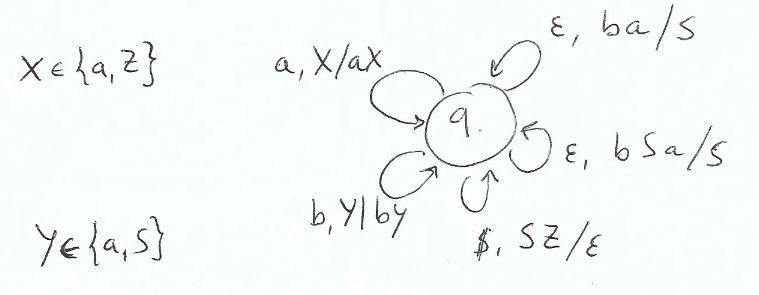
\includegraphics[width=0.7\textwidth]{img/esempio38.png}
\end{center}
  \begin{center}
    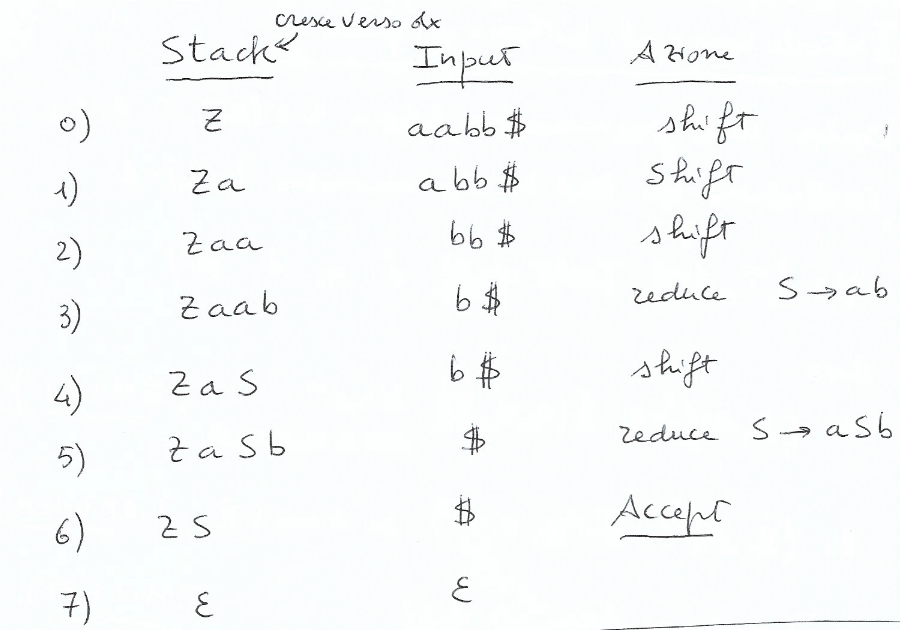
\includegraphics[width=0.7\textwidth]{img/esempio39.png}
\end{center}
Derivazione canonica destra a rovescio:
\begin{align*}
  aabb \leftarrow aSb \leftarrow S
\end{align*}
  \begin{center}
    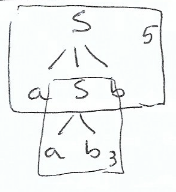
\includegraphics[width=0.2\textwidth]{img/esempio40.png}
\end{center}
  \begin{center}
    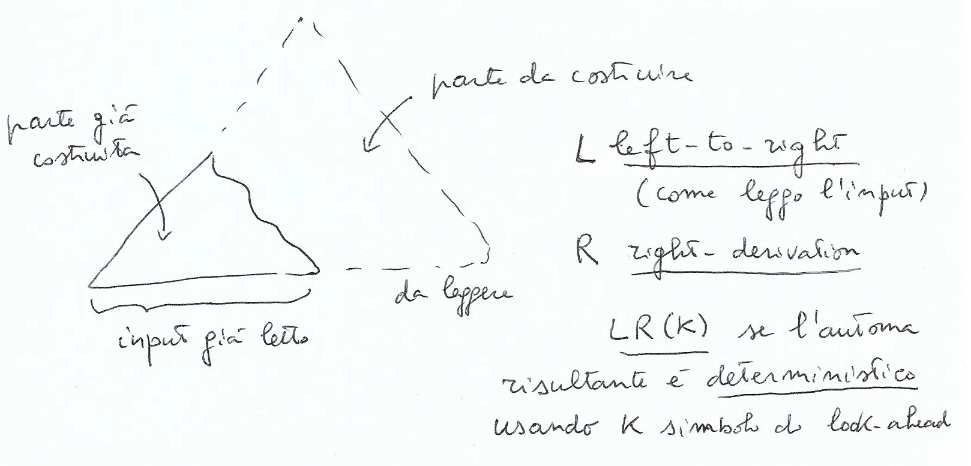
\includegraphics[width=0.7\textwidth]{img/esempio41.png}
\end{center}
C'e' molto nondetermismo!
\begin{itemize}
  \item conflitti \textit{shift-reduce}
  \begin{itemize}
    \item 3) $Zaab \quad b\mathdollar$ 
    \item 4') $Zaabb \quad \mathdollar$ 
  \end{itemize}
  potrei fare shift ma e' un percorso infruttuoso
  \item conflitti \textit{reduce-reduce} \\
  (possibili solo con grammatiche piu' complete)
\end{itemize}
$\to$ Per ottenere un DPDA serve introdurre informazioni aggiuntive per risolvere i conflitti
\begin{itemize}
  \item piu' stati \\
  (o strutture particolari di supporto alla decisione: DFA dei prefissi visibili)
  \item look-ahead \\
  (guardare l'input in avanti)
\end{itemize}
Vediamo un esempio piu' corposo relativo alla grammatica delle espressioni aritmetiche
\begin{align*}
  E \to T+E \mid T \\
  T \to T*A \mid A \\
  A \to a \mid b \mid (E)
\end{align*}
  \begin{center}
    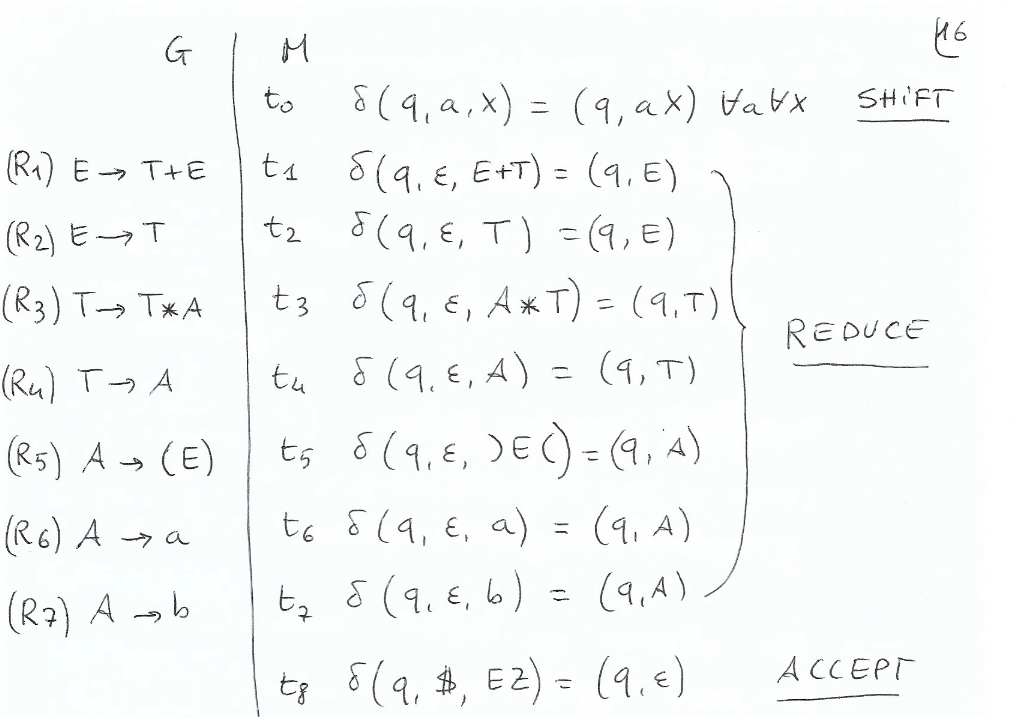
\includegraphics[width=0.7\textwidth]{img/esempio42.png}
\end{center}
\begin{align*}
  a*(b) \leftarrow A*(b) \leftarrow T*(b) \leftarrow T * (A) \leftarrow T*(T) \leftarrow T * (E) \leftarrow T * A \leftarrow T \leftarrow E
\end{align*}
derivazione canonica dx a rovescio (\textit{rigthmost})
  \begin{center}
    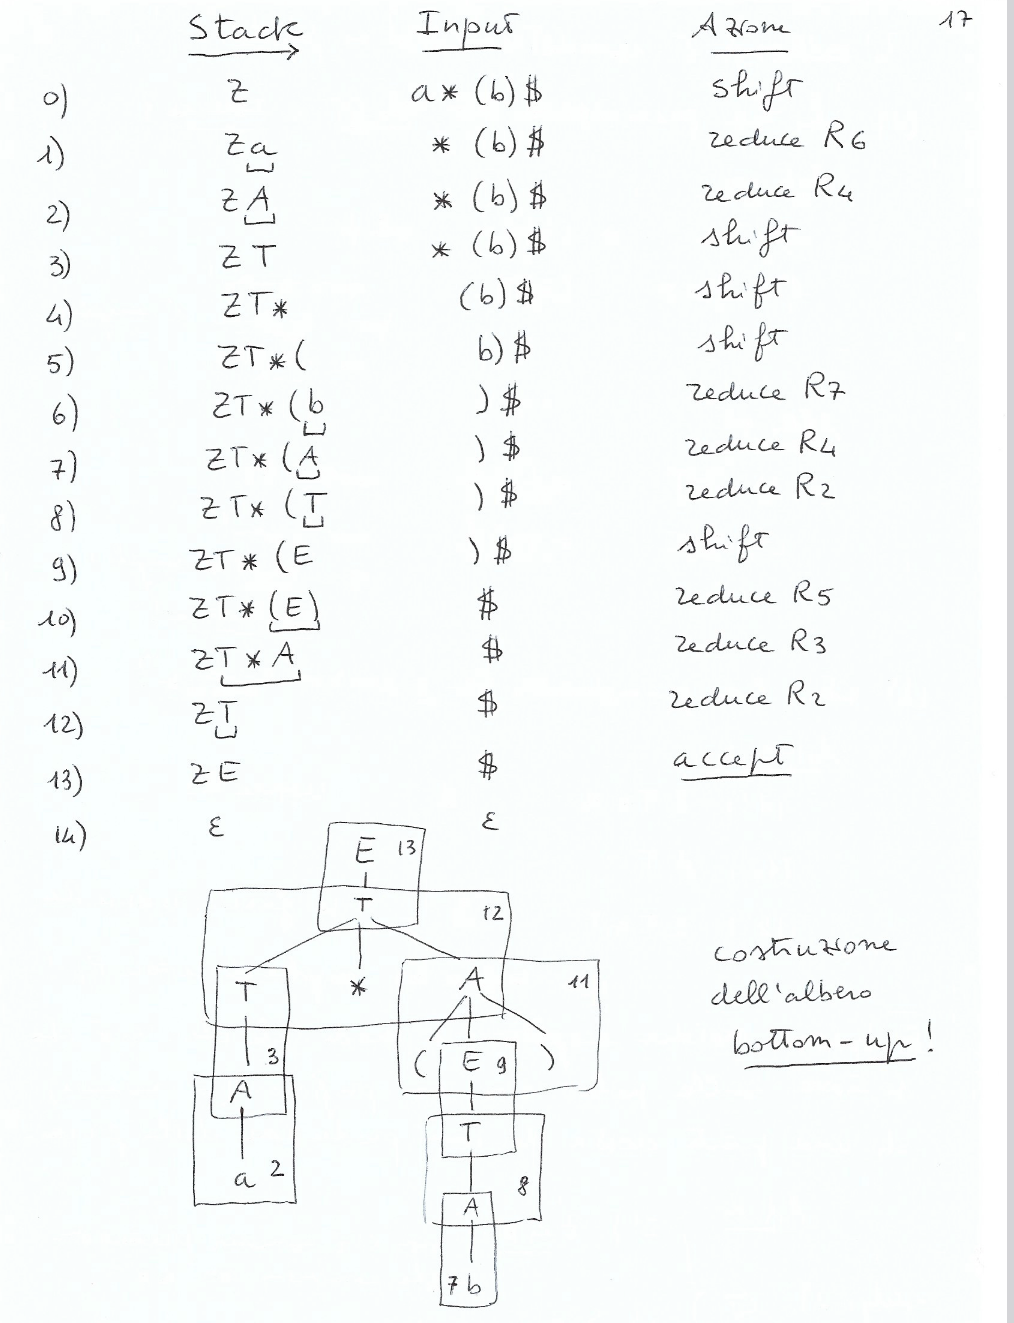
\includegraphics[width=0.7\textwidth]{img/esempio43.png}
\end{center}
L'automa e' non deterministico perche'
\begin{itemize}
  \item chi ha precedenza tra shift e reduce? \\
  Ad esempio:
  \begin{itemize}
    \item 1) $za \quad *(b)\mathdollar$ 
    \item 2') $za* \quad (b)\mathdollar$ 
  \end{itemize}
  shift non buono! Qui reduce e' meglio di shift!
  \item chi ha la precedenza tra 2 diverse reduce? \\
  Ad esempio:
  \begin{itemize}
    \item (11) $zT * A \quad \mathdollar$ reduce $R_3$
    \item (12) $zT$
    \item (12') $zt*T \quad \mathdollar$ se faccio reduce $R_4$
  \end{itemize}
  Qui reduce $R_3$ meglio di reduce $R_4$!
\end{itemize}
E' buona norma scegliere un modo tale che cio' che si trova sulla pola sia un prefisso (a rovescio) di una parte destra di una produzione della gramamtica!!!
  \begin{center}
    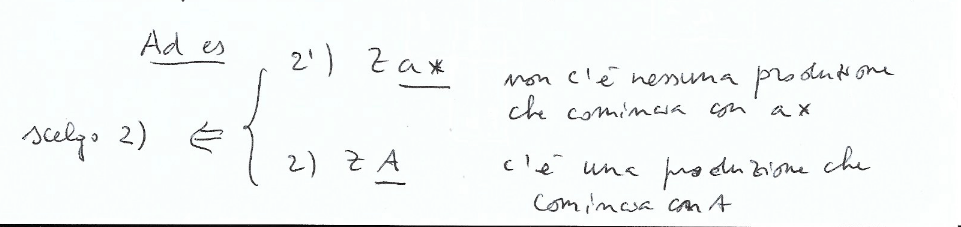
\includegraphics[width=0.9\textwidth]{img/esempio44.png}
\end{center}
\subsection*{Problema con produzione $\epsilon$ del tipo $A \to \epsilon$}
  \begin{center}
    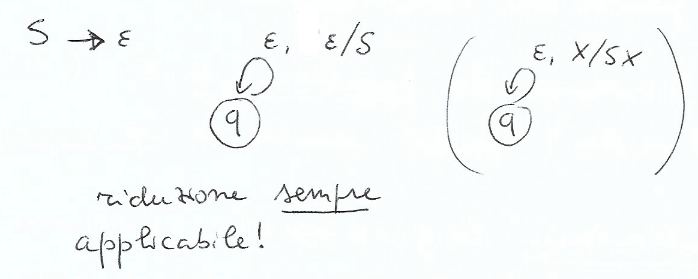
\includegraphics[width=0.6\textwidth]{img/esempio45.png}
\end{center}
$\to$ cercare di evitare di usare grammatiche libere con produzioni $\epsilon$ quando si vuole usare la tecnica di bottom-up parsing (shift-reduce).
\section{Semplificare le grammatiche}
Per avere PDA piu' efficienti/piccoli e con minor nondeterminismo e' necessario semplificare le grammatiche.
\begin{itemize}
  \item Eliminare le produzioni $\epsilon$ (del tipo $A \to \epsilon$) che sono indatte al bottom-up parsing
  \item Eliminare le produzioni unitarie (del tipo $A \to B$) che possono creare cicli $A \to^+ A$
  \item Eliminare simboli inutili, cioe' quei terminale e nonterminali che non sono raggiungibili/generabili a partire dal simbolo iniziale S
  \item Eliminare la ricorsione sinistra (del tipo $A \to A\zeta$), perche' inadatta al top-down parsing
  \item Fattorizzare la grammatica per ottenere grammatiche con meno nondeterminismo nel top-down parsing
\end{itemize}
\subsection{Eliminare le produzione $\epsilon$}
\begin{itemize}
  \item Input: $G$ libera con produzione $\epsilon$ (del tipo $A \to \epsilon$)
  \item Output: $G$ libera senza produzioni $\epsilon$ tale che 
  \begin{align*}
    L(G')=L(G)\backslash \{\epsilon\}
  \end{align*}
\end{itemize}
\textit{Osservazione}: Se $\epsilon \in L(G)$ e vogliamo una $G''$ tale che $L(G)=L(G'')$ basta considerare $\underbrace{G'}_\text{output dell'algoritmo} = (NT, T, S, R')$  definire $G''=G' \cup \{S' \to \epsilon \mid S\}$
\begin{align*}
  G''=(NT \cup \{S'\}, T, S', R' \cup \{S' \to \epsilon \mid S\})
\end{align*}
\vspace{1em}
\textbf{Simbolo annulabile}: $A \in NT$ tale che $A \to^+ \epsilon$ \\
$N(G) = \{A \in NT \mid A \to^+ \epsilon\}$ viene calcolato induttivamente come segue: \\
$N_0(G) = \{A \in NT \mid A\to \epsilon \in R\}$ \\
$N_{i+1} = N_i(G) \cup \{B \in NT \mid B \to C_1 \dots C_k \in R \text{ e } c_1,\dots,c_k \in N_i(G)\}$ \\
\textit{Osservazione}: 
\begin{itemize}
  \item $N_i(G) \subseteq N_{i+1}(G)$ perche' aggiungo qualcosa ad ogni passo
  \item $\exists i_c$ tale che $N_{i_c}(G)=N_{i_{c+1}}(G)$ perche' $NT$ e' finito! \\
\end{itemize}
\textit{Fatto}: L'insieme $N(G) = N_{i_c}(G)$ e' esattamente l'insieme di tutti i simbolo annulabili. \\
Una volta calcolato $N(G)$ per $G = (NT, T, S, R)$ costruiamo la grammatica $G' = (NT, T, S, R')$ dove per ogni produzione $A \to \zeta \in R$ con $\zeta \neq \epsilon$ (1) in cui occorrono i simboli annullabili $z_1, \dots, z_k$ mettiamo in $R'$ tutte le produzioni del tipo $A\to \zeta'$ dove $\zeta'$ si ottiene da $\zeta$ cancellando tutti i possibili sottoinsiemi di $z_1, \dots, z_k$ (incluso $\emptyset$) ad eccezione del caso in cui $\zeta'$ risulta $\epsilon$ (2)
\begin{itemize}
  \item 1) in $G'$ non mettiamo produzioni $A\to \epsilon \in R$
  \item 2) in $G'$ non introduciamo mai produzioni del tipo $A\to \epsilon$
\end{itemize}
\textit{Proposizione}: Data una grammatica libera $G$ la grammatica $G'$ determinata dall'algoritmo sopra non ha $\epsilon \text{-produzioni}$ e $L(G') = L(G) \backslash \{\epsilon\}$
  \begin{center}
    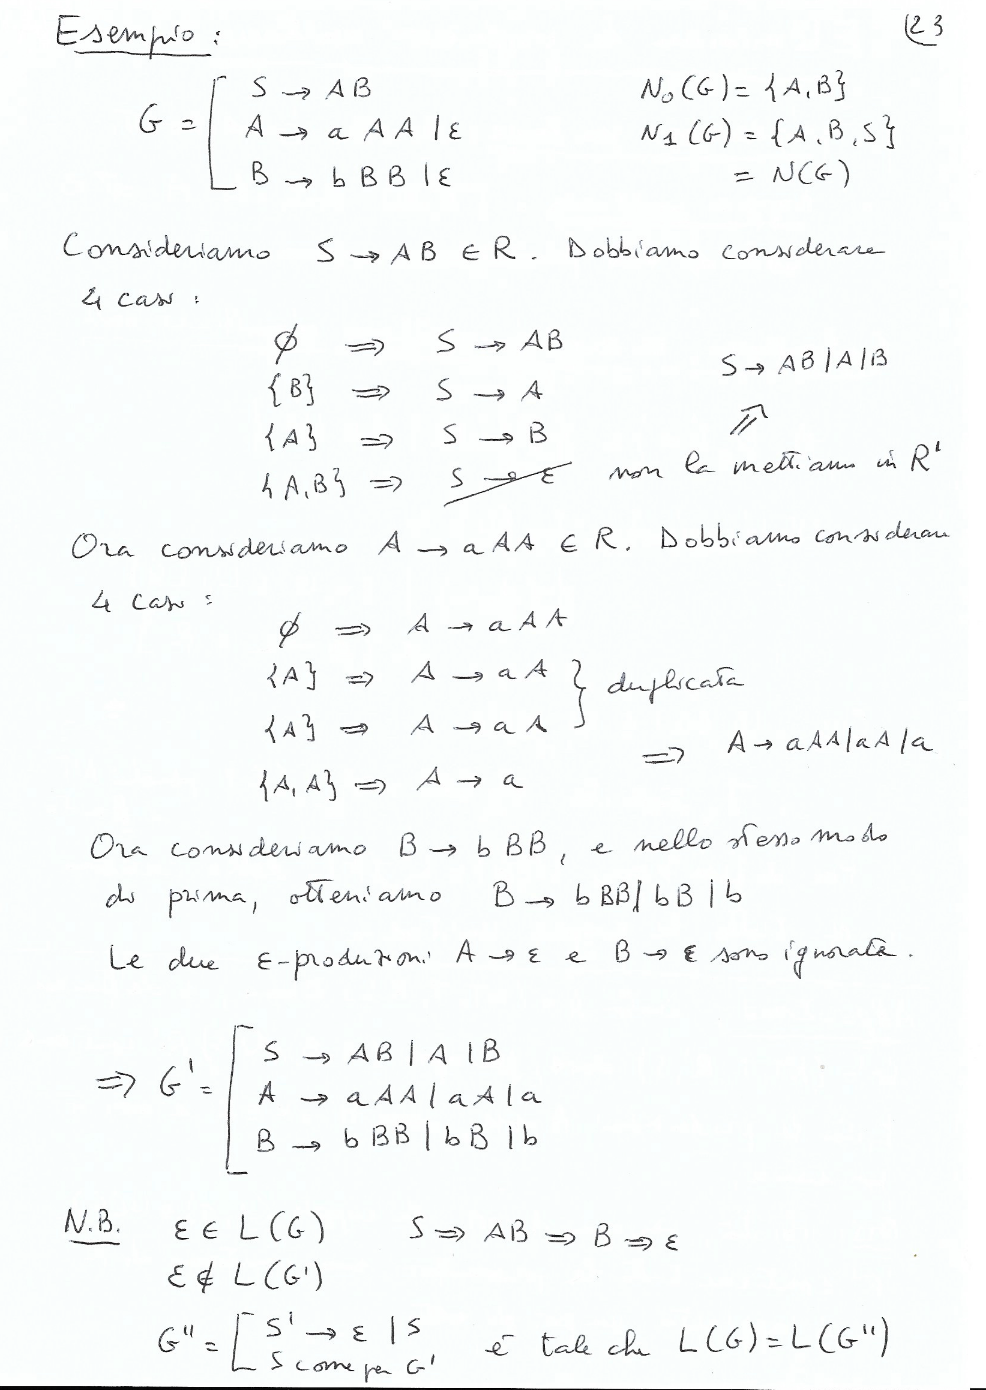
\includegraphics[width=0.9\textwidth]{img/esempio46.png}
\end{center}
\subsection{Eliminare le produzioni unitarie}
\begin{itemize}
  \item produzioni unitarie: $A\to B$ con $A, B \in NT$
  \item coppie unitarie: $(A,B)$ tale che $A \to^* B$ usando solo produzioni unitarie
\end{itemize}
\textbf{Calcolare le coppie unitarie induttivamente}
\begin{itemize}
  \item 1) $U_0(G) = \{(A,A) \mid A \in NT\}$
  \item 2) $U_{i+1}(G) = U_i(G)\cup \{(A,C) \mid (A,B) \in U_i(G) \text{ e } B \to C \in R\}$
\end{itemize}
\textit{Osservazione}: $U_i (G) \subseteq U_{i+1}(G)$
\begin{itemize}
  \item $\exists i_c$ tale che $U_{i_c}(G) = U{i_c +1}(G)$ perche' $NT$ e' finito
\end{itemize}
Per definizione $U(G)=U_{i_c}(G)$ detto insiem di tutte le coppie unitarie. \\
\vspace{1em} \\
\textit{Algorimto}: Data $G = (NT, T, R, S)$ libera si definisce $G'(NT, T, R', S)$ dove per ogni $(A,B) \in U(G)$ $R'$ contiene tutte le produzioni $A \to \zeta$ dove $B \to \zeta \in R$ e non e' unitaria. \\
\textit{Osservazione}: Poiche' per ogni $A \in NT$ la coppia $(A,A) \in U(G)$, $R'$ contiene tutte le produzioni non unitarie di $R$ e in aggiunta un po' di altro. \\
\vspace{1em} \\
\textbf{Teorema}: \\
Sia $G = (NT, T, R, S)$ libera e sia $U(G)$ l'insieme delle sue coppie unitarie. Sia $G' = (NT, T, R', S)$ la grammatica ottenuta dall'algoritmo sopra. Allora $G'$ non ha produzioni unitarie e $L(G) = L(G')$.
  \begin{center}
    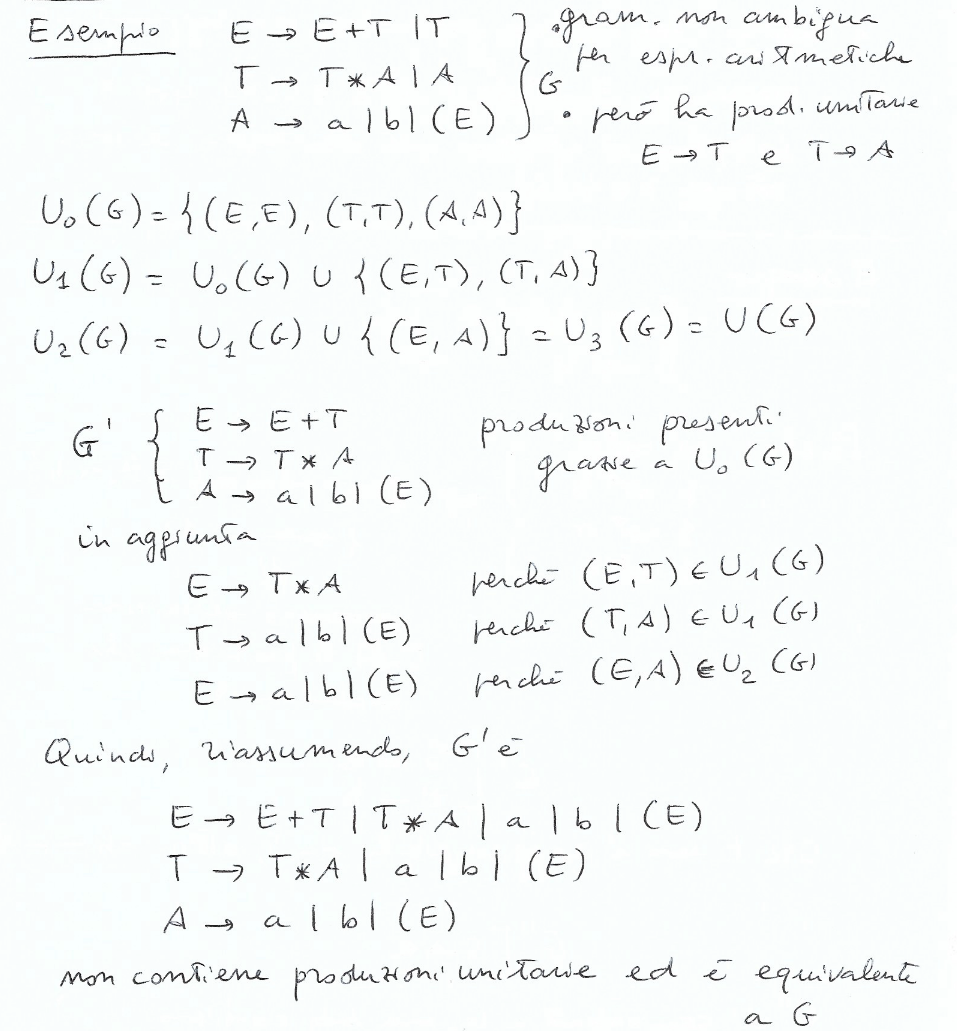
\includegraphics[width=0.7\textwidth]{img/esempio47.png}
\end{center}
\subsection{Rimuore i simboli inutili}
\textit{Definizione}: Un simbolo $x \in T \cup NT$ e'
\begin{itemize}
  \item un generatore sse $\exists w \in T^*$ con $x \to^* w$
  \item raggiungibile sse $S \to^* \zeta xB$ per qualche $\zeta, B \in (T \cup NT)^*$
  \item utile sse sia generatore, sia raggiungibile ovvero se $S \to^* \zeta xB \to^* z \in L(G)$ cioe' $x$ compare in almeno una derivazione di una stringa $z \in L(G)$
\end{itemize}
  \begin{center}
    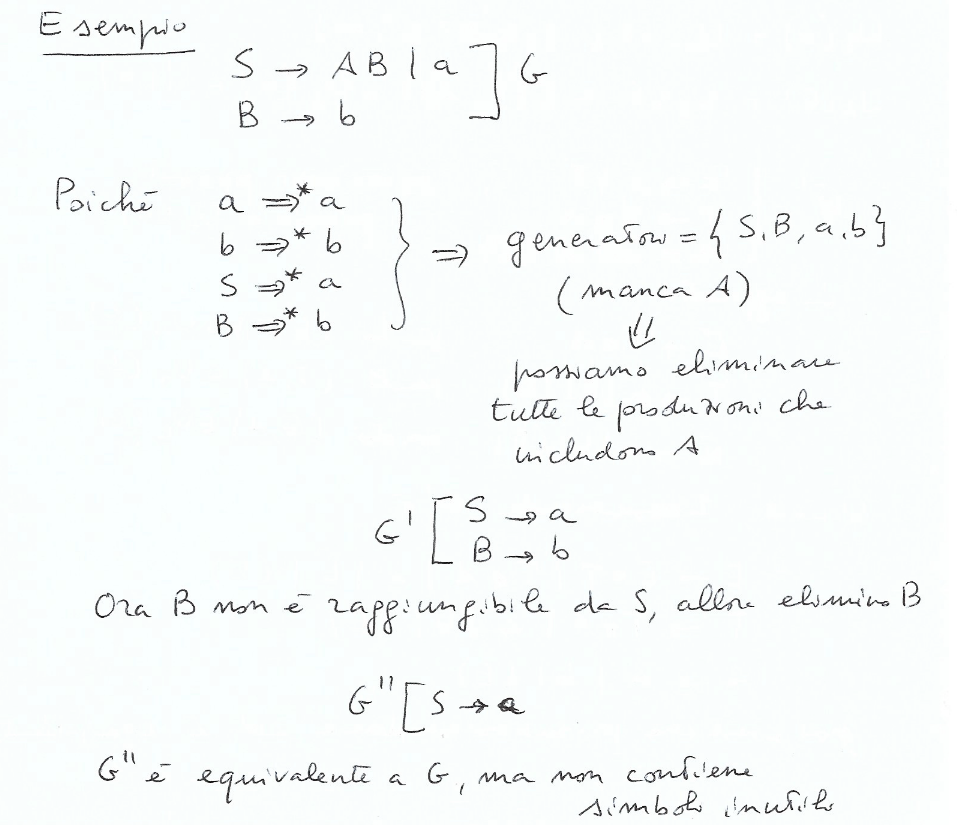
\includegraphics[width=0.7\textwidth]{img/esempio48.png}
\end{center}
\subsection{Come calcolare i generatori?}
Ricorda: $x$ e' generatore sse $\exists w \in T^* \quad x \to^* w$
\begin{itemize}
  \item 1) $G_0(G) = T\quad $ (se $a \in T, \quad a \to^* a$! allora tutti i terminali sono generatori)
  \item 2) $G_{i+1}(G) = G_i(G) \cup \{B \in NT \mid B \to c_1, \dots, c_k \in R \text{ e } c_1, \dots, c_k \in G_i(G)\}$
\end{itemize}
\textit{Osservazione}: Nel passo \textit{2} e' contemplato anche il caso $k=0$ (cioe' $B \to \epsilon \in R$): se $B \to \epsilon$, allora $B$ e' un generatore. \\
\textit{Osservazione}: 
\begin{itemize}
  \item $G_i(G) \subseteq G_{i+1}(G)$
  \item $\exists i_c$ tale che $G_{i_c}(G) = G_{i_c + 1}(G)$ perche' $T \cup NT$ e' finito
\end{itemize}
\textit{Fatto}: L'insieme $G(G) = G_{i_c}(G)$ e' esattamente l'insieme di tutti i simboli generatori di $G$. \\
\vspace{1em} \\
\subsection{Come calcolare i raggiungibili?}
\textit{Ricorda}: $x$ e' raggiungibile sse $S \to^* \zeta xB$ per qualche $\zeta, B \in (NT \cup T)^*$
\begin{itemize}
  \item 1) $R_0(G)=\{S\}$
  \item 2) $R_{i+1}(G)=R_i(G) \cup \bigcup_{B \in R_i(G),\quad  B \to x_1, \dots, x_k \in R}\{x_1, \dots, x_k\}$
\end{itemize} 
\textit{Osservazione}: 
\begin{itemize}
  \item $R_i (G) \subseteq R_{i+1}(G)$
  \item $\exists i_c \cdots R_{i_c}(G) = R_{i_c +1}(G)$ perche' $T \cup NT$ e' finito
\end{itemize}
\textit{Fatto}: L'insieme $R(G) = R_{i_c}(G)$ e' esattamente l'insieme di tutti i simboli raggiungibili di $G$. \\
\vspace{1em} \\
\subsection{Come rimuovere i simboli inutili?}
\begin{itemize}
  \item Prima elimino tutti i non-generatori (e tutte le produzioni che usano almeno uno di questo)
  \item Poi della nuova grammatica elimino tutti i non-raggiungibili (e tutte le produzione che li usano)
\end{itemize}
$\to$ La grammatica risultanete e' equivalente all'originale e non cotiene simboli inutili. \\
\vspace{1em} \\
\subsection{Eliminare i simboli inutili}
\textit{Teorema}: Sia $G = (NT, T, R, S)$ una grammatica libera tale che $L(G) \neq \emptyset$
\begin{itemize}
  \item Sia $G_1$ la grammatica che si ottiene da $G$ eliminando tutti i simboli che non appartengono a $G(G)$ e tutte le produzioni che fanno uso di almeno uno di tali simboli $\circledast$.
  \item Sia $G_2$ la grammatica che si ottiene da $G_1$ eliminando tutti i simboli che non appartengono a $R(G_1)$ e tutte le produzioni che fanno uso di almeno uno di tali simboli.
\end{itemize}
Allora $G_2$ non ha simboli inutili e $L(G_2) = L(G)$. \\
\textit{Dimostrazione}: (Lez13-Gorrieri.pdf slide 10) \\
\vspace{1em} \\
\subsection*{L'ordine dei 2 passi e' importante!}
\begin{itemize}
  \item 1) prima elimino i non-generatori
  \item 2) poi i non raggiungibili
\end{itemize}
Ma se inverto l'ordine allora puo' capitare che non elimino tutti i simboli inutili! 
\subsection*{Mettere le cose insieme $\dots$}
Se nel semplificare la grammatica $G$ seguiamo questo ordine:
\begin{itemize}
  \item 1) eliminiamo le $\epsilon$-produzioni
  \item 2) eliminare le produzioni unitarie (e quindi i cicli)
  \item 3) eliminare i simboli inutili
\end{itemize}
allora la gramamtica risultante e' garantita non avere ne $\epsilon$-produzioni, ne produzioni unitarie, ne simbolo inutili, ed e' equivalente a quella di partenza! \\
\textit{N.B.}: L'ordine e' importante poiche' alcune delle costruzioni possono interagire tra loro!  \\
\vspace{2em} \\
\subsection{Forme normali}
\begin{itemize}
  \item di Chomsky
  \item di Grenbach
\end{itemize}
garantiscono proprieta' particolari alla grammatica. \\
\vspace{10px} \\
\subsection*{Forma normale di Chomsky}
Tutte le produzioni sono della forma (con $\epsilon$ trattato a parte: $S \to \epsilon \mid BC \dots$) ($S$ non compare mai a dx in una produzione)
\begin{align*}
  A \to BC \\
  A \to a
\end{align*}
\textit{Osservazione}: se $G$ libera e' in forma normale di Chomsky allora
\begin{itemize}
  \item non ha $\epsilon$-produzioni
  \item non ha produzioni unitarie
\end{itemize}
\textit{Osservazioni}: Ogni grammatica libera $G$ puo' essere trasformata in una equivalente $G'$ in forma normale di Chomsky. \\
\vspace{10px} \\
\subsection*{Forma normale di Grenbach}
Tutte le produzioni sono della forma (con $\epsilon$ trattato a parte come sopra)
\begin{align*}
  A \to aBC \\
  A \to aB \\
  A \to a
\end{align*}
\textit{Osservazione}:
\begin{itemize}
  \item no $\epsilon$-produzioni / no produzioni unitarie
  \item non e' mai ricorsiva a sx!
  \item ogni produzione applicata in una derivazione allunga in prefisso di termninali $\to$ parser costruiti a partire da forma normale di Grenbach  sono meno nondeterminismo. 
\end{itemize}
\textit{Osservazione}: Ogni $G$ libera puo' essere trasformata in una equivalenza $G'$ forma normale di Grenbach. \\
\vspace{1em} \\
\subsection{Eliminare la ricorsione sinistra}
(problema del parser top-down)
\begin{itemize}
  \item produzione ricorsiva sx: $A \to A \zeta \in R$
  \item $G$ e' ricorsiva sx: $A \to^+ A\zeta$ per qualche $A \in NT$ e $\zeta \in (T \cup NT)^*$
\end{itemize}
\subsection*{Come rimuove la ricorsione sx immediatamente?}
\begin{align*}
  A \to A \zeta_1 \mid \dots \mid A \zeta_n \mid B_1 \mid \dots \mid B_m
\end{align*}
(le stringhe $B_i$ non cominciamo per $A$) \\
Queste produzioni possono essere rimpiazzate da 
\begin{align*}
  A \to B_1 A' \mid \dots \mid B_m A' \\
  A' \to \zeta_1 A' \mid \dots \mid \zeta_n A' \mid \epsilon
\end{align*}
Se nella grammatica originale abbiamo la derivazione
\begin{align*}
  A \to A \zeta_{i_1} \to A \zeta_{i_2}\zeta_{i_1} \to \dots \to A\zeta_{i_k} \dots \zeta_{i_2}\zeta_{i_1} 
\end{align*}
allora nella nuova grammatica avremo 
\begin{align*}
  A \to B_i A' \to B_i \zeta_{i_k}A' \to \dots \to B_i \zeta_{i_k} \dots \zeta_{i_2} \to B_i \zeta_{i_k}\dots\zeta_{i_2}\zeta_{i_1}A' \\
  \to B_i \zeta_{i_k}\dots \zeta_{i_2}\zeta_{i_1}
\end{align*}
e viceversa. \\
\subsection*{Ricorsione sx non-immadiate}
Consideriamo
  \begin{center}
    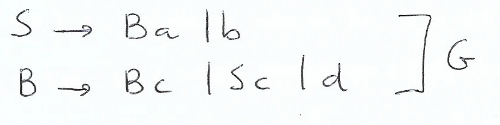
\includegraphics[width=0.3\textwidth]{img/esempio49.png}
\end{center}
In $G$ c'e' ricorsione sx immadiate ($B \to Bc$), ma anche non-immediate ($S \to Ba \to Sca$). \\
\vspace{2em}\\
\textit{Algorimto}: 
\begin{itemize}
  \item input: $G$ libero senza $\epsilon$-produzioni, senza produzioni unitarie, ma con ricorsione sx non-immediata
  \item $G'$ libero, senza ricorsione sx, ma puo' avere $\epsilon$-produzioni
\end{itemize}
Sia $NT = \{A_1, A_2, \dots, A_n\}$ in ordine fissato
\begin{itemize}
  \item For $i$ from $1$ to $n$
  \begin{itemize}
    \item 1) For $j$ from $1$ to $i-1$
    \begin{itemize}
      \item sostituisci ogni produzione della forma $A_i \to A_j \zeta$ con produzioni $A_i \to B_1 \zeta \mid \dots \mid B_k \zeta$ dove $A_j \to B_1 \mid \dots \mid B_k$ sono le produzioni correnti per $A_j$
    \end{itemize}
    \item 2) Eliminare la ricorsione immediata su $A_i$
  \end{itemize} 
\end{itemize} 
\vspace{1em}
\begin{itemize}
  \item L'obbiettivo dell'algoritmo e' che alla fine ogni produzione del tipo $A_i \to A_{k^\zeta}$ sia tale che $i < k$ in modo che sia impossibile avere ricorsione sx non immediata.
  \item Quando $i=1$ l'unica cosa che viene fatta e' l'istruizione \textit{2} che rimuove l'eventuale sicorsione sx immediata, Al termine se $A_1 \to A_{k^\zeta}$ avremo $1 < k$.
  \item Alla $i$-esima iterazione del \textit{for} esterno tutti i nonterminali $A_m$ con $m < i$ hanno produzioni con la proprieta' desiderata. Ora il ciclo \textit{for} interno (istruizione \textit{1}) aumenta progressivamente l'indice del nonterminale in prima posizione, finche', al termine del ciclo ($j = i-1$) avremo che ogni produzione $A_i \to A_{k^\zeta}$ e' tale che $i \leq k$. Ora l'istruzione \textit{2} rimuove l'eventuale ricorsione sx immediata da $A_i$ sicche' ogni produzione $A_i \to A_{k^\zeta}$ e' tale che i $i < k$.
  \item Quindi al termine dell'algortimo ($i = n$) avremo che ogni produzione $A_i \to A_{k^\zeta}$ e' tale che $i < k$, garantendo l'impossibile di creare ricorsione sx non immediata.
  \begin{align*}
    NT = \{\underbrace{S}_\text{1}, \underbrace{B}_\text{2}\} \\
    S \to Ba \mid b \\
    B \to Bc \mid Sc \mid d
  \end{align*}
  \item Per $i=1$ (cioe' per $S$) il ciclo interno ($j$ da 1 a $\emptyset$) non viene eseguito. Siccome non c'e' ricorsione immediata per S non faccio niente!
  \item Per $i=2$ (cioe' per $A_i=B$) il ciclo interno ($j$ da 1 a 1) si esegue solo per $A_j = A_1 = S$. Allora la produzione $B \to Sc$ viene rimpiazzata con 
  \begin{align*}
    B \to Bac \mid bc
  \end{align*}
  Ora le produzioni complessive per $B$ sono
  \begin{align*}
    B \to Bc \mid Bac \mid bc \mid d
  \end{align*}
  delle quali dobbiamo eliminare la ricorsione immediate! Il risultato e'
  \begin{align*}
    B \to bcB' \mid dB' \\
    B' \to cB' \mid acB' \mid \epsilon 
  \end{align*}
  ovvero la grammatica risultante e'
  \begin{align*}
    S \to Ba \mid b \\
    B \to bcB' \mid dB' \\
    B' \to cB' \mid acB' \mid \epsilon
  \end{align*}
\end{itemize}
Poiche' si richiedere che la $G$ in input non abbia produzioni unitarie e produzioni $\epsilon$?
  \begin{center}
    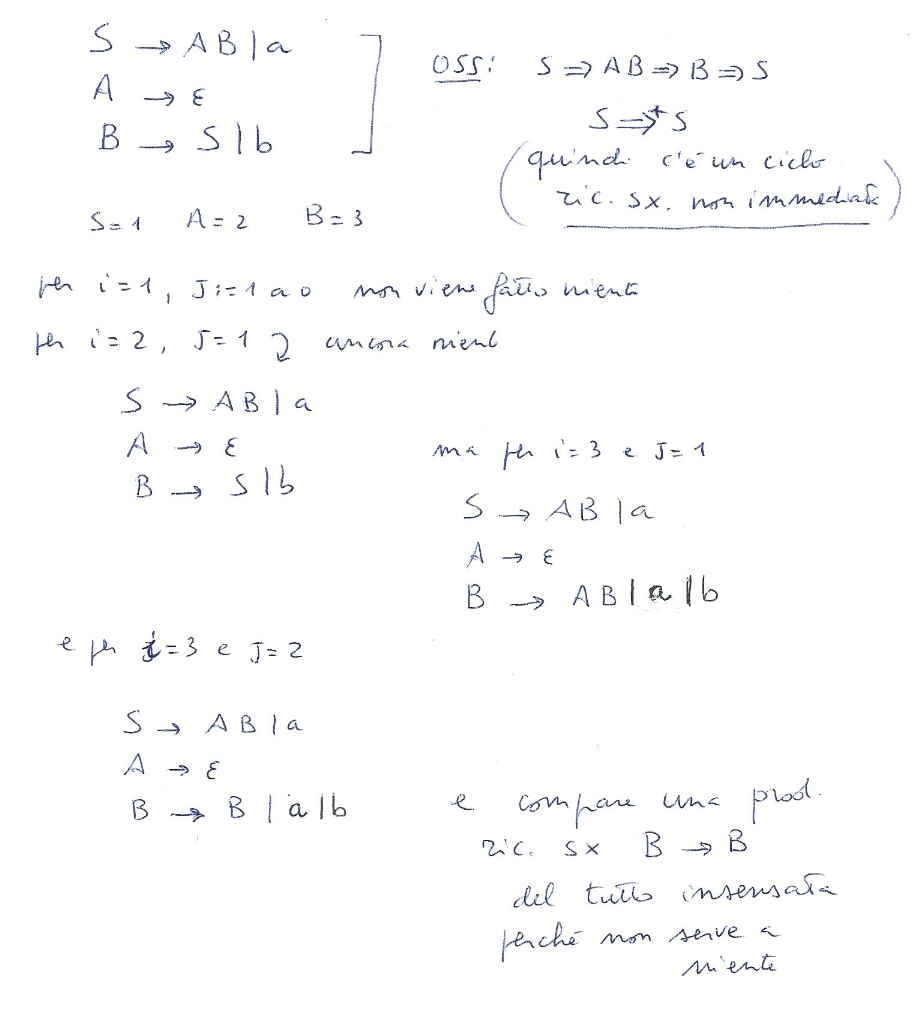
\includegraphics[width=0.7\textwidth]{img/esempio50.png}
\end{center}
\vspace{1em}
\subsection*{Fattorizzazione a sinistra}
(importante nel top-down parsing)
\begin{align*}
  A \to aBbC \mid aBd
\end{align*}
Se in top-down parsing sulla pila ha $A$ e leggo in input $a$ non sono in grado di determinare quale produzione sciegliere (nondeterminismo) \\
$\to$ raccolgo la parte comune ("$aB$") alle 2 produzioni e introduco un nuovo nonterminale per rappresentare il "resto"
\begin{align*}
  A \to aBA' \\
  A' \to bC \mid d
\end{align*}
\textbf{Algoritmo generale}:
\begin{itemize}
  \item Inizializza $N = NT$
  \item Ripeti il ciclo presente finche' nessuna modifica e' piu' possibile a $N$ o all'insieme delle produzioni
  \begin{itemize}
    \item for each $a \in N$
    \begin{itemize}
      \item Sia $\zeta$ il prefisso piu' lungo comune alla parti destre di alcune produzioni di $A$;
      \item if $\zeta \neq \epsilon$
      \begin{itemize}
        \item sia $A'$ un nuovo nonterminale; $N = N \cup \{A\}$;
        \item rimpiazzare tutte le produzioni $A$
        \begin{align*}
          A \to \zeta B_1 \mid \dots \mid \zeta B_k \mid y_1 \mid \dots \mid y_h
        \end{align*}
        con le produzioni
        \begin{align*}
          A \to \zeta A' \mid y_1 \mid \dots \mid y_h \\
          A' \to B_1 \mid \dots \mid B_k
        \end{align*}
      \end{itemize}
    \end{itemize}
  \end{itemize}
\end{itemize}
  \begin{center}
    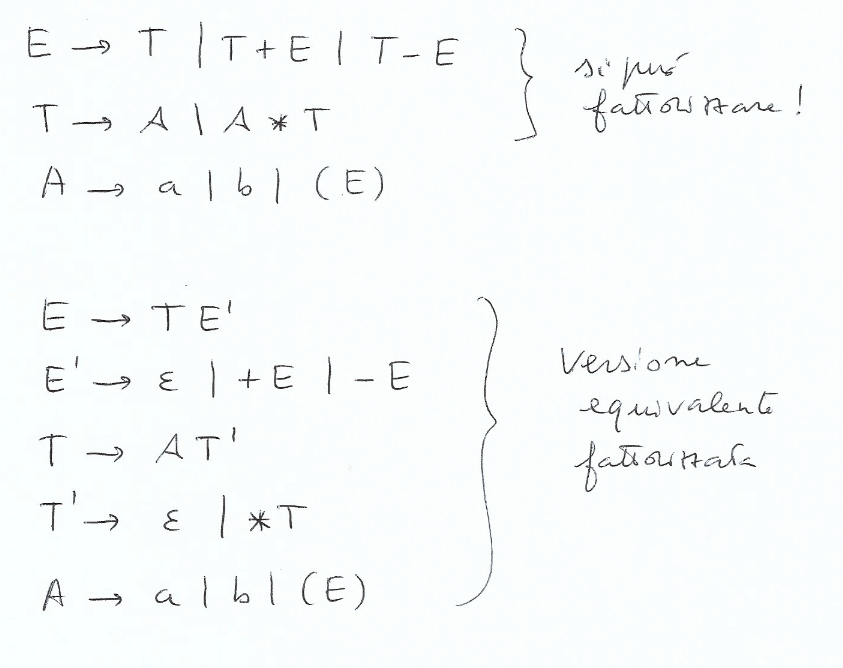
\includegraphics[width=0.7\textwidth]{img/esempio51.png}
\end{center}
\vspace{1em}
\section{Parser top-down}
Presentiamo un primo esempio di parser top-down nondeterministico che usa implicitamente una pila per gestire le chiamate ricorsive. \\
\vspace{5px}\\
Data una grammatica $G = (NT, T, S, R)$ pe rogni nonterminale $A$ con produzioni
\begin{align*}
  A \to x_1^1 \dots x_{n1}^1 \mid \dots \mid x_1^k \dots x_{nk}^k
\end{align*}
definisce la funzione
\begin{itemize}
  \item function A()
  \begin{itemize}
    \item 1) scegli nondetermisticamente $h$ tra $1$ e $k$, ovvero una produzione $A \to x_1^h \dots x_{nh}^h$;
    \item 2) for $i=1$ to $n_h$
    \begin{itemize}
      \item if $x_i^h \in NT$ then $x_i^h()$;
      \item else if $x_i^h = \text{"simbolo corente dell'input"}$ then avanza di un simbolo sull'input;
      \item else \textit{fail()}; //backtracking si torna al punto \textit{1} e si sceglie un altra posizione
    \end{itemize}
  \end{itemize}
  \item return;
\end{itemize}
Si comincia incovando la funzione per il simbolo iniziale $S$. \\
\vspace{1em} \\
\subsection*{Parser a discesa ricorsiva}
e' molto inefficiente:
\begin{itemize}
  \item Nondeterminismo:
  \begin{itemize}
    \item necessita' di esplorare nel caso tutte le alternative! \\
    $\to$ esponenziale nella lunghezza della stringa $w$ dove la base $b$ e' data dal massimo numero di produzione per uno stesso nonterminale 
    \begin{align*}
      O(b^{\mid w \mid})
    \end{align*}
  \end{itemize}
  $\to$ Cerchiamo di guidare la scelta della produzione! Guardando il prossimo/i carattere dell'input da leggere.
\end{itemize}
\textit{Attenzione}: da qui in poi assumiamo di avere un simbolo speciale $\mathdollar$ che non faccia parte dei simboli di nessuna grammatica, che useremo come segnalatore di fine input! \\
\textbf{Perche'?} Un parser top-down e' alla fine un DPDA che riconosce per pila vuota. Allora e' necessario che L goda della prefix propriety e $L \cdot \mathdollar$ sicuramente gode di questa proprieta'. \\
\vspace{1em} \\
\subsection{First}
Data una grammatica libera $G$ e $\zeta \in (T \cup NT)^*$ diciamo che $First(\zeta)$ e' l'insieme dei terminale che possono stare in prima posizione in una stringa che si deriva da $\zeta$.
\begin{itemize}
  \item per $a \in T, \quad a \in First(\zeta)$ sse $\zeta \to^* aB$ per $B \in (T \cup NT)^*$
  \item inoltre se $\zeta \to^* \epsilon$ allora $\epsilon \in First(\zeta)$ 
\end{itemize} 
\vspace{1em}
\subsection{Follow}
Data una grammatica libera $G$ e $A \in NT$ diciamo che $Follow(A)$ e' l'insieme dei terminali che possono comparire immediatamente a destra di $A$ in una forma sentenziale
\begin{itemize}
  \item per $a \in T, \quad a \in Follow(A)$ sse $S \to^* \zeta AaB$ per qualche $\zeta, B \in (T \cup NT)^*$
  \item $\mathdollar \in Follow(A)$ se $S \to^* \zeta A$
\end{itemize}
  \begin{center}
    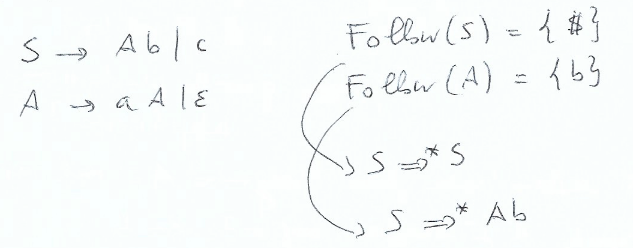
\includegraphics[width=0.6\textwidth]{img/esempio52.png}
\end{center}
\subsection*{Come calcolare i First?}
Sia $N(G) \subseteq NT$ l'insieme dei simboli annullabili ($A \in N(G)$ sse $A \to^* \epsilon$)
\begin{itemize}
  \item Per ogni $x \in NT, \quad First(x)=\{x\}$
  \item Per ogni $x \in NT,$ inizializza $First(x) = \emptyset$
  \item Ripeti il seguente ciclo finche' nessun $First(x)$ viene piu' modificato in una iterazione:
  \begin{itemize}
    \item Per ogni produzione $x \to y_1 \dots y_k$
    \begin{itemize}
      \item per ogni $i$ da $1$ a $k$
      \begin{itemize}
        \item se ($y_1, \dots, y_{i-1} \in N(G)$) //true se $i=1$
        $\quad$ allora $First(x) \, := \, First(x) \cup (First(y_i) \backslash \{\epsilon\})$
      \end{itemize}
    \end{itemize}
  \end{itemize}
  \item Per ogni $x \in N(G), \quad First(x) \, := \, First(x) \cup \{\epsilon\}$
\end{itemize}
\vspace{1em} 
$First$ puo' essere esteso ad $\zeta \in (T \cup NT)^*$ come segue:
\begin{itemize}
  \item $First(\epsilon)=\{\epsilon\}$
  \item $First(xB) = First(x)$ se $x \notin N(G)$
  \item $First(xB) = (First(x) \backslash \{\epsilon\}) \cup First(B)$ se $x \in N(G)$
\end{itemize}
In pratica se $A \to \zeta_1 \mid \dots \mid \zeta_k$ allora 
\begin{align*}
  First(A) = First(\zeta_1) \cup \dots \cup First(\zeta_k)
\end{align*}
  \begin{center}
    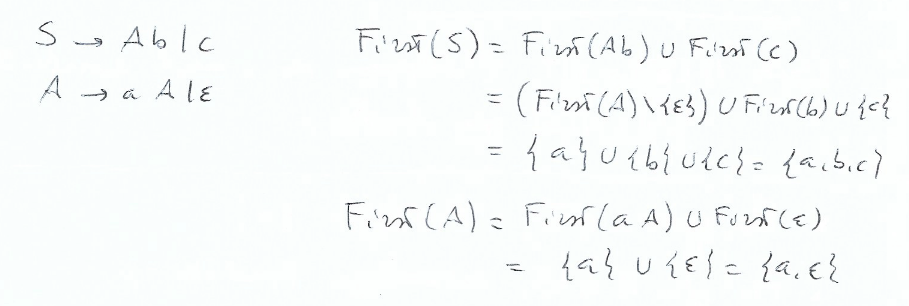
\includegraphics[width=0.7\textwidth]{img/esempio53.png}
\end{center}
\subsection*{Procedure per calcolare $Follow(x)$ (con $x \in NT$)}
\begin{itemize}
  \item Per ogni $x \in NT$ iniziallizza $Follow(x) \, := \, \emptyset$
  \item $Follow(S) \, := \ \{S\}$
  \item Ripeti il seguente ciclo finchè nessun $Follow(x)$ viene più modificato in una iterazione:
  \begin{itemize}
    \item 1) Per ogni produzione $x \to \zeta yB$ \\
    $\quad Follow(y) \, := \, Follow(y) \cup (First(B) \backslash \{\epsilon\})$
    \item 2) Per ogni produzione $x \to \zeta y$ e per ogni produzione $x \to \zeta yB$ con $\epsilon \in First(B)$ \\
    $\quad Follow(y)\, := \, Follow(y) \cup Follow(x)$
  \end{itemize}
\end{itemize}
In pratica bisogna cercare tutte le produzioni in cui $x \in NT$ appare e per ognuna di esse applicare la \textit{1} o \textit{2} sopra. \\
\vspace{1em} \\
\subsection{Tabella di parsing LL(1)}
\begin{align*}
  \underbrace{\text{Tabella}}_\text{strumento per risolvere il nondetermismo} \text{ di parsing } \underbrace{\text{L}}_\text{input left-to-right} \underbrace{\text{L}}_\text{derivazione leftmost} \underbrace{\text{(1)}}_\text{un simbolo di look-ahead}
\end{align*}
\textbf{Matrice bidimensionale M}
\begin{itemize}
  \item righe: nonterminali
  \item colonne: terminali (più $\mathdollar$)
  \item casella ($A, a$): $M[A,a]$ contiene le produzioni che possono essere scelte dal parser mentre tenta di espandere $A$ e se l'input corrente è $a$
\end{itemize}
Se ogni casella contiene al più una produzione allora il parser è deterministico! \\
\textbf{Come si riempe la tabella?} \\
Per ogni produzione $A \to a$:
\begin{itemize}
  \item 1) per ogni $a \in T$ e $a \in First(\zeta)$, inserisce $A \to \zeta$ nella casella $M[A,a]$
  \item 2) se $\epsilon \in First(\zeta)$ inserisci $A \to \zeta$ in tutte le caselle $M[A,x]$ per $x \in Follow(A)$ ($x$ può essere $\mathdollar$)
\end{itemize}
Ogni casella vuota dopo aver elaborato tutte le produzioni è un errore (cioè la funzione ricorsiva chiama $fail()$). \\
\vspace{1em} \\
\textit{Definizione}: Una grammatica è LL(1) sse ogni casella della tabella di parsing LL(1) contiene al più una produzione. \\
\textbf{Parser "predittivo" deterministico}: se $G$ è LL(1) allora il parser ricostruisce l'albero di derivazione per l'input $w$ in modo top-down predicendo quale produzione usare (tra le molte possibili) guardando il prossimo carattere dell'input. \\
\vspace{1em} \\
\textit{Teorema}: $G$ è LL(1) sse ogni coppia di produzioni distinte con la stessa testa
\begin{align*}
  A \to \zeta \mid B
\end{align*}
si ha che
\begin{itemize}
  \item $First(\zeta) \cap First(B) = \emptyset$
  \item a) se $\epsilon \in First(\zeta)$ allora $First(B) \cap Follow(A) = \emptyset$
  \item b) se $\epsilon \in First(B)$ allora $First(\zeta) \cap Follow(A) = \emptyset$
\end{itemize}
\textit{Dimostrazione}: Se sono soddisfatte le condizioni \textit{1} e \textit{2} per ogni coppia di produzioni distinte con medesima testa, allora la tabella di parsing LL(1) contiene al più una produzione in ogni casella! Ma vale anche viceversa! \\
\vspace{1em} \\
\subsection{Parser LL(1) non ricorsivo}
(usando esplicitamente una pila)
\begin{itemize}
  \item Pila $:= \, S \mathdollar$; (cima della pila a sinistra)
  \item $x \, := \, w \mathdollar$; (top della pila)
  \item input $:= \, w \mathdollar; \quad i_c = \text{primo carattere dell'input}$;
  \item while($x \neq \mathdollar$)
  \begin{itemize}
    \item if ($x$ è un terminale)
      \begin{itemize}
        \item 1) if ($x \, := \, i_c$)
          \begin{itemize}
            \item pop $x$ dalla pila; avanza $i_c$ dall'input;
          \end{itemize}
        \item else $errore()$; %caso no match
        \item 2) $x \, := \, $ top della pila
    \end{itemize}
    \item else
      \begin{itemize}
        \item 1) if ($M[x, i_c] = x \to y_1 \dots y_n$)
              \begin{itemize}
                \item pop $x$ dalla pila;
                \item push $y_1 \dots y_n$ sulla pila ($y_1$ in cima)
                \item output la produzione $x \to y_1 \dots y_n$
              \end{itemize}  
        \item else $errore()$ %caso "bianco"
        \item 2) $x \, := \, $ top della pila;
      \end{itemize}  
  \end{itemize}
  \item if ($i_c \neq \mathdollar $) $errore()$; % caso "ho svuotato la pila ma non ho finitol'input!"
\end{itemize}
  \begin{center}
    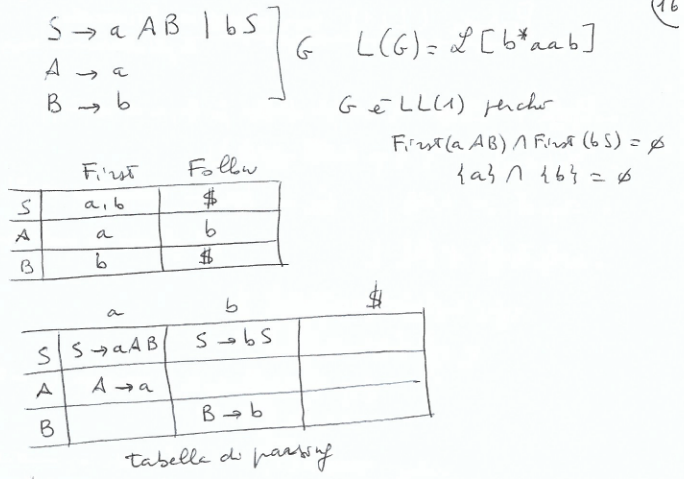
\includegraphics[width=0.7\textwidth]{img/esempio54.png}
\end{center}
  \begin{center}
    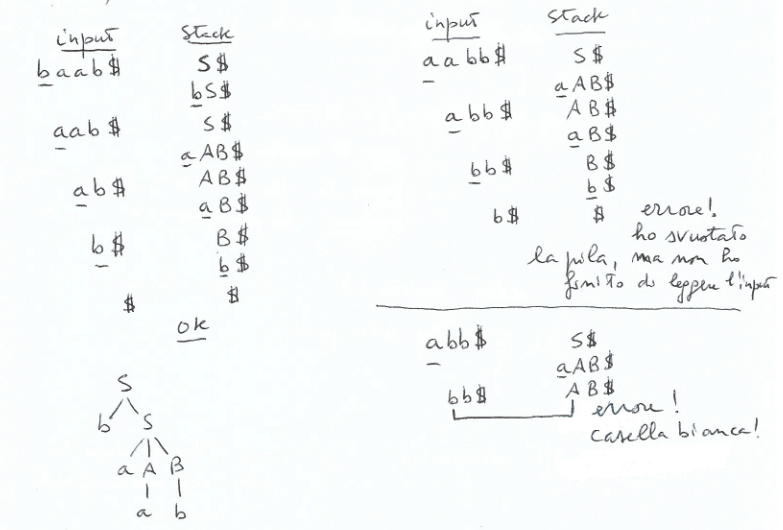
\includegraphics[width=0.7\textwidth]{img/esempio55.png}
\end{center}
\vspace{1em}
\textit{Teorema}: Ogni linguaggio regolare è generabile da una grammatica $G$ di classe LL(1). \\
\textit{Dimostrazione}: (Lez14-Gorrieri.pdf slide 19) \\
\vspace{2em} \\
\subsection{Grammatiche LL($k$)}
\begin{itemize}
  \item $\dfrac{First_k(\zeta)}{w \in First_k(\zeta)}$ sse $\zeta \to^* wB$ con $\mid w \mid = k, \quad w \in T^*, \quad B \in (T \cup NT)^*$ oppure $\zeta \to^* w$ con $\mid w \mid \leq k, \quad w \in T^*$
  \item $\dfrac{Follow_k(A)}{w \in Follow_k(A)}$ sse $S \to^* \zeta A wB$ con $\mid w \mid = k$ e $w \in T^* \quad \zeta, B \in (T \cup NT)^*$ oppure $S \to^* \zeta Aw$ con $\mid w \mid \leq k$ e $w \in T^*$
\end{itemize}
Tabella di parsing LL($k$)
\begin{itemize}
  \item righe: nonterminali
  \item colonne: $\{w \in T^* \mid \quad \mid w \mid \leq k\}$ (solo quelle necessarie)
  \item Per ogni produzione $A \to \zeta, M[A, w]$ contiene $A \to \zeta$ per ogni $w \in First_k(\zeta) \quad (w \neq \epsilon)$ e per ogni $w \in Follow_k(A)$ se $\epsilon \in First_k(\zeta)$
  \item Se ogni entrata/casella contiene al più una produzione,e non esistono $w_1$ e $w_2$ tale che $w_1$ prefisso di $w_2$ con le due entrate corrispondenti su una riga entrambe riempite allora $G$ è LL($k$).
\end{itemize}
\textit{N.B.}: Le colonne sono tante quanti i $w$ che appartengono a $First_k(\zeta) $ per $A \to \zeta$ o a $Follow_k(A)$ per $A \to \zeta$ (se $\epsilon \in First_k(\zeta)$). E questo va fatto per tutte le produzioni! \\
\vspace{1em} \\
\textit{Teorema}:
\begin{itemize}
  \item Una grammatica ricorsiva sinistra non è LL($k$) per nessun $k$.
  \item Una grammatica ambigua non è LL($k$) per nessun $k$.
  \item Se $G$ è LL($k$) per qualche $k$ allora $G$ non è ambigua!
  \item Se $G$ è LL($k$) allora $L(G)$ è libero deterministo!
  \item Esiste $L$ libero deterministo tale che non esiste $G$ di classe LL($k$) per nessun $k$ tale che $L = L(G)$
\end{itemize}
  \begin{center}
    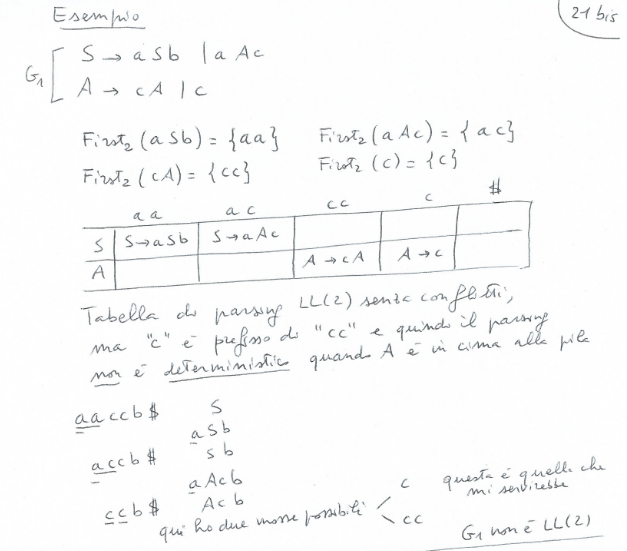
\includegraphics[width=0.9\textwidth]{img/esempio56.png}
\end{center}
\textit{Definizione}: Un linguaggio $L$ è di classe $LL(k)$ se esiste $G$ di classe $LL(k)$ tale che $L = L(G)$. \\
\textit{Proposizione}: Per ogni $k \geq 0$ la classi di linguaggio $LL(k+1)$ contiene strettamente la classe di linguaggi $LL(k)$.
  \begin{center}
    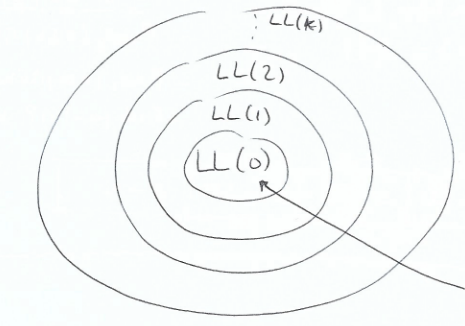
\includegraphics[width=0.4\textwidth]{img/esempio57.png}
\end{center}
\textbf{In pratica si usa solo $LL(1)$}! Se $G$ non è $LL(1)$ spesso la si può manipolare (fattorizzare, elininare ricorsione sx, disambiguare, ecc) trasformandola in una equivalente $LL(1)$ \\
\vspace{1em} \\
\section{Parser bottom-up}
(o \textit{shift-reduce})
\begin{itemize}
  \item shift: un simbolo terminale viene spostato dall'input sulla pila
  \item reduce: una serie di simboli (terminali e nonterminali) sulla cima della pila corrisponde al "reverse" di una parte destra di una produzione 
  \begin{align*}
    A \to \zeta \in R \quad - \quad \zeta^R \text{ sulla pila}
  \end{align*}
  La stringa $\zeta^R$ viene rimossa dalla pila e sostituita con $A$ ("$\zeta$ viene ridotta ad $A$")
\end{itemize}
Riprendiamo ora la presentazione di un parser \textit{shift-reduce} nondeterministico, che è essenzialmente un PDA con un solo stato che riconosce per pila vuota il linguaggio $L \cdot \mathdollar$ \\
\textbf{Parser LR}:
\begin{itemize}
  \item L (leggo da sx a dx)
  \item R (derivazione rightmost)
\end{itemize}
\vspace{1em}
\subsection{Parser shift-reduce nondetermismo}
\begin{itemize}
  \item Input:
  \begin{itemize}
    \item una grammatica libera $G$ con simbolo iniziale $S$
    \item una stringa $W \in T^*$
  \end{itemize}
  \item Output:
    \begin{itemize}
    \item se $w \in L(G)$ allora restituisce la sua derivazione rightmost a rovescio
  \end{itemize}
\end{itemize}
\vspace{1em}
  \begin{itemize}
    \item Inizializziamo la pila a $\mathdollar$;
    \item Inizializziamo l'input con $w \mathdollar$;
    \item Usiamo il PDA seguente per trovare la derivazione per $w \mathdollar$
    \begin{align*}
      M = (T, \{q\}, \underbrace{T \cup NT \cup \{\mathdollar\}}_\Gamma, \delta, \mathdollar, \emptyset)
    \end{align*}
    dove 
    \begin{itemize}
      \item 1) $(q, ax) \in \delta(q, a, x) \quad \forall a \in T \quad \forall x \Gamma$ (SHIFT) 
      \item 2) $(q, A) \in \delta(q, \epsilon, \zeta^R)$ se $A \to \zeta \in R$ (REDUCE)
      \item 3) $(q, \epsilon) \in \delta(q, \mathdollar, S \mathdollar)$ (ACCEPT)
    \end{itemize}
    \item ogni volta che facciamo "REDUCE" forniamo in output la produzione usata
    \item alla fine $S \mathdollar$ sulla pila con $\mathdollar$ in input.
    \begin{center}
    $\to$ Ok, accettiamo
    \end{center}
  \end{itemize}
    \begin{center}
    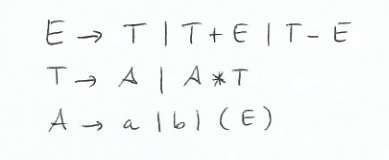
\includegraphics[width=0.4\textwidth]{img/esempio58.png}
\end{center}
  \begin{center}
    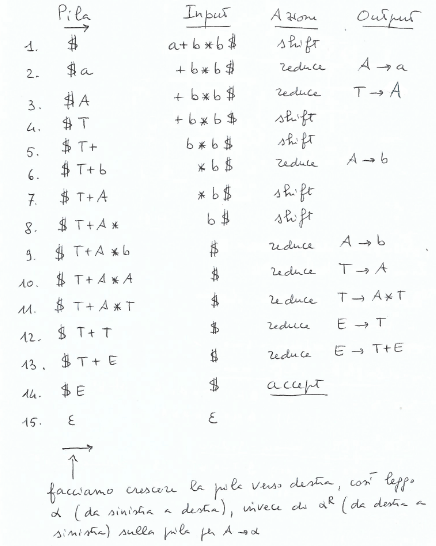
\includegraphics[width=0.7\textwidth]{img/esempio59.png}
\end{center}
  \begin{center}
    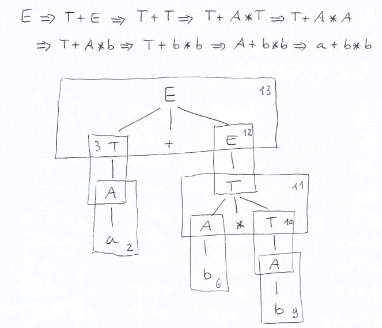
\includegraphics[width=0.7\textwidth]{img/esempio60.png}
\end{center}
\begin{itemize}
  \item costruizione dell'albero di derivazione bottom-up
  \item derivazione canonica destra a rovescio
  \item enorme nondetermismo
  \begin{itemize}
    \item conflitti shift-reduce
      \begin{itemize}
      \item 2') $\mathdollar a \quad +b*b\mathdollar$ shift
      \item 3') $\mathdollar a+ \quad b*b\mathdollar$
  \end{itemize}  
  \item conflitti reduce-reduce
    \begin{itemize}
    \item 11') $\mathdollar T+A*T \quad \mathdollar$ reduce $T \to T$
    \item 12') $\mathdollar T+A*E \quad \mathdollar$
  \end{itemize}  
  \end{itemize}  
\end{itemize}
\vspace{1em}
\subsection{Come risolvere i conflitti?}
  \begin{itemize}
    \item Strategia: bisogna scegliere l'azione giusta in un modo che sulla pila ci sia un prefisso viabile
  \end{itemize}  
\textit{Prefisso viabile}: è una sequenza $ \in (T \cup NT)^*$ che può apparire sulla pila di un parser bottom-up per computazione che accetta un input. \\
In pratica bisogna che la parte top della pila sia un prefisso di una parte dx di una produzione \\
Nei 2 esempi precedenti:
  \begin{itemize}
    \item $\mathdollar a+$ non è un prefisso di parte dx di una produzione mentre $\mathdollar a$ lo è!
    \item $\mathdollar T+A*E$ non è un prefisso di una parte dx di una produzione mentre $\mathdollar T+T$ lo è!
  \end{itemize}  
Quindi dovremo fornire al PDA per renderlo deterministico una struttura di controllo (tabella di parsing) che ci aiuti a scegliere l'azione giusta. \\
\vspace{1em} \\
\subsection{Come è fatto un parser LR?}
  \begin{center}
    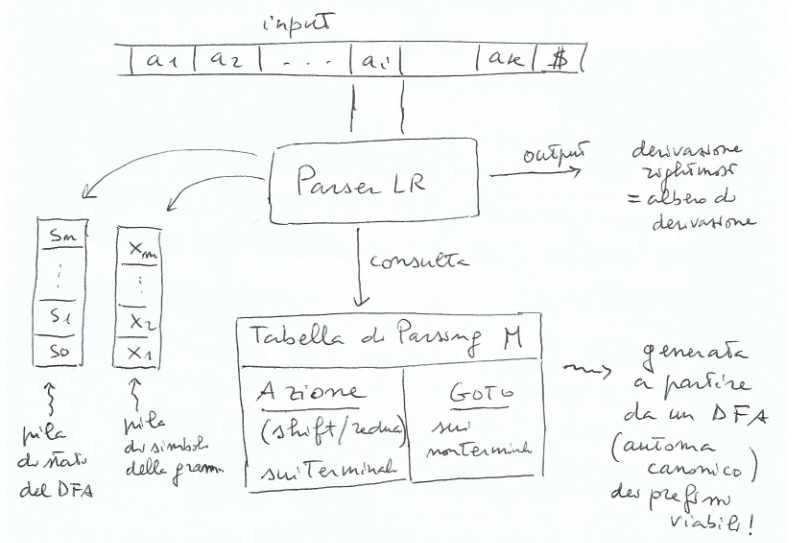
\includegraphics[width=0.7\textwidth]{img/esempio61.png}
\end{center}
Una configurazione di un parser LR è
\begin{align*}
  (\underbrace{S_0 \dots S_n}_\text{stack degli stati}, \underbrace{x_1 \dots x_m}_\text{stack dei simboli}, \underbrace{a_i \dots a_k}_\text{resto dell'input} \mathdollar)
\end{align*}
\textit{Osserva}: "$x_1 \dots x_m \, a_i \dots a_k$ è una stringa intermedia della derivazione canonica destra" \\
\vspace{1em} \\
\subsection{Mosse del parser LR}
\begin{itemize}
  \item 1) Prima legge: $[\underbrace{\text{stato top}}_{S_n} \text{ e } \underbrace{\text{simboli contenuti dell'input}}_{a_i}]$
  \item 2) consulta la tabella di parsing LR $M[S_n \, a_i]$
  \begin{itemize}
    \item se $M[S_n a_i]= \text{shifts}$, allora la nuova configurazione è
    \begin{align*}
      (S_0 \dots S_n,\,  x_1 \dots x_m, \, a_{i+1} \dots a_k \mathdollar )
    \end{align*}  
    \item se $M[S_n a_i]= \text{reduce} A \to B$, allora la nuova configurazione è
    \begin{align*}
      (S_0 \dots S_{n-r} S, x_1 \dots x_{m-r} A, a_i \dots a_k \mathdollar)
    \end{align*}
    dove $r = \mid B \mid$ e $M[S_{n-r}, A] = \text{goto s}$, cioè fa tre passi:
    \begin{itemize}
      \item faccio "pop" di $r$ elementi dai 2 stack
      \item metto $A$ in cima alla pila di simboli
      \item calcolo il nuovo stato top, guardando $M[S_{n-r}, A] = \text{goto s}$ e metto $S$ in cima alla pila degli stati
    \end{itemize}
    \item se $M[S_n, a_i] = \text{accept} \to \text{Fine!}$
    \item se $M[S_n, a_i] = \text{"bianco"} \to \text{errore!}$
  \end{itemize}
\end{itemize}
  \begin{center}
    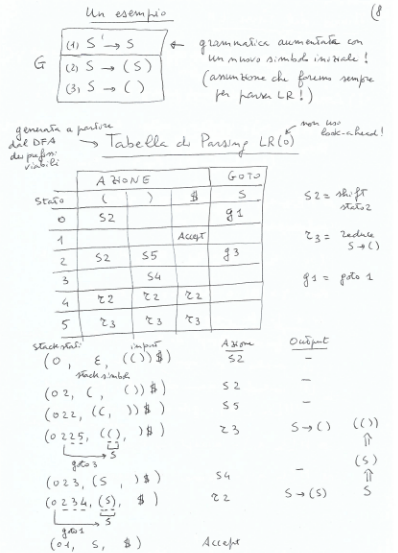
\includegraphics[width=0.9\textwidth]{img/esempio62.png}
\end{center}
\subsection{DFA dei prefissi viabili / Automa canonico LR(o)}
  \begin{center}
    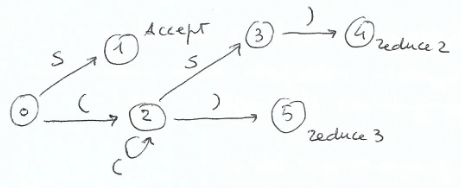
\includegraphics[width=0.5\textwidth]{img/esempio63.png}
\end{center}
\begin{itemize}
  \item da questo DFA (che non è esattamente un DFA!) si ricava la tabella di parsing LR(o)
  \item ma come si ricava questo DFA a partire dalla grammatica? (lo vedremo tra poco)
\end{itemize}
Le operazione shift-reduce devono far si che rimanga in cima alla pila un prefisso di una parte dx di una produzione! Nel suo complesso la pila deve contenere un prefisso di derivazione canonica dx! \\
Nell'esempio:
\begin{itemize}
  \item appena sulla pila compare ")" allora dobbiamo fare una reduce \\
  Quale reduce fare, dipende dalla "storia", ovvero dallo stato su cui ci siamo finito sul DFA
\end{itemize}
\vspace{1em} 
\subsection{Prefisso viabile}
\textit{Definizione 1}: Un prefisso viabile è una stringa $\in (T \cup NT)^*$ che può apparire sulla pila di un parser bottom-up per una computazione che accetta input. \\
\textit{Definizione 2}: (su grammatica libera) Una stringa $y \in (T \cup NT)^*$ è un prefisso variabile per $G$ sse esiste una derivazione rightmost
\begin{align*}
  S \to^* SAy \to \delta \zeta B y = \gamma By
\end{align*}
per qualche $y \in T^*, \delta \in (T \cup NT)^*$ e per una produzione $A \to \zeta B$. Inoltre $S$ è un prefisso variabile per definizione. Un prefisso variabile è completo se $B = \epsilon$; in tal caso $\zeta$ è detta \texttt{maniglia} (handle) per $\gamma y$, (ovvero in cima alla pila trovo $\zeta^R$ e posso fare una reduce) \\
\vspace{5px} \\
Come fare a:
\begin{itemize}
  \item riconoscere le maniglie sulla cima della pila e ridurle?
  \item scegliere tra più riduzioni solo quelle che producono sulla pila un nuovo prefisso variabile?
  \item scegliere spostamenti che completino i prefissi viabili sulla pila e facciano comparire una nuova maniglia?
\end{itemize}
\textit{Teorema}: Data $G$ libera i prefissi variabili di $G$ costruiscono un linguaggio regolare e può essere descritto con un DFA. \\
$\to$ Il parser (cioè un PDA) può consultare il DFA dei prefissi viabili (ovvero la tabella di parsing) per decidere cosa fare.
\begin{itemize}
  \item se la pila contiene un prefisso variabile completo, allora il parser riduce;
  \item se la pila contiene un preficco variabile incompelto, allora il parser shifta;
  \item se la pila non contiene un prefisso variabile, allora errore;
\end{itemize}
A seconda di come è fatto il DFA il parser può risultare deterministico o meno. (eventualmente sfruttando informazioni di look-ahead e sui follow dei nonterminali per ottenere determinismo) \\
\vspace{1em} \\
Anche se, concettualmente, ad ogni modifica della pila il DFA le riscandisce da capo per determinare come sia fatto il prefisso variabile corrente, questo non è necessario perchè ad ogni prefisso di un prefisso viabile è un prefisso viabile! \\
La pila viene modificata in 2 modi:
\begin{itemize}
  \item shift: la pila passa da $\mathdollar \gamma $ a $\mathdollar \gamma x$. In tal caso il DFA si trova nello stato $S$ dopo aver elaborato $\mathdollar y \to$ basta far ripartire il DFA da $S$ con input $x$.
  \item reduce $A \to \zeta$: la pila passa da $\mathdollar \gamma \zeta$ a $\mathdollar \gamma A$. In tal caso il DFA si trova nello stato $S$ dopo aver elaborato $\mathdollar \gamma \zeta$; non c'è bisogno di far ripartire il DFA dalla base della pila; basta ripristinare lo stato in cui si trovava subito prima di elaborare il primo simbolo di $\zeta$ e fornirgli il simbolo $A$ in input.
\end{itemize}
$\to$ mi servo lo stack degli stati del DFA!!! \\
(anzi mi basterebbe solo lo stack degli stati; ma noi usiamo anche lo stack di simboli per ragioni didattiche) \\
\vspace{1em} \\
\textbf{Uno stato del DFA dei prefissi variabili} (chiamato automa canonico LR(o)) è costituito da un insieme di item LR(o) \\
ITEM LR(o): è una produzione con indicata, con un punto, una posizione della sua parte destra. \\
\vspace{5px} \\
ES 1: $A \to xyz$ genera 4 item
\begin{align*}
  A \to .xyz \\
  A \to x.yz \\
  A \to xy.z \\ 
  A \to xyz.
\end{align*}
Il punto "." indica parte della produzione è già stata analizzata 
\begin{itemize}
  \item se $A \to \zeta . B$ è nello stato del DFA in cima alla pila, allora vuol dire che $\zeta$ è sulla pila dei simboli e che ci si aspetta che l'input da leggere contenga (o possono venir ridotti a) $B$ \\
  \item se $A \to \zeta .$ è nello stato del DFA in cima alla pila, allora sulla pila dei simboli c'è la maniglia $\zeta$ e possiamo fare la reduce
\end{itemize}
\vspace{1em} 
\subsection{Come costruire l'NFA dei prefissi vaibili?}
Data $G = (NT, T, S, R)$ libera prendiamo la grammatica aumentata con un nuovo simbolo iniziale $S'$ ed una produzione $S' \to S$. \\
L'\textit{NFA dei prefissi viabili di $G$} (primo passo verso la costruzione del DFA!) si ottiene così:
\begin{itemize}
  \item $[S' \to .S]$ è lo stato iniziale
  \item dallo stato $[A \to \zeta .xB]$ c'è una transizione allo stato $[A \to \zeta x.B]$ eticchettato $x$, per $x \in T \cup NT$
  \item dallo stato $[A \to \zeta .xB]$, per $x \in NT$ e per ogni produzione $X \to y$ c'è una $\epsilon-$tranzione verso lo stato $[x \to .y]$  
\end{itemize}
\textit{Osservazione}: non serve definire degli stati finali perchè l'NFA serve solo come ausilio al parser. 
  \begin{center}
    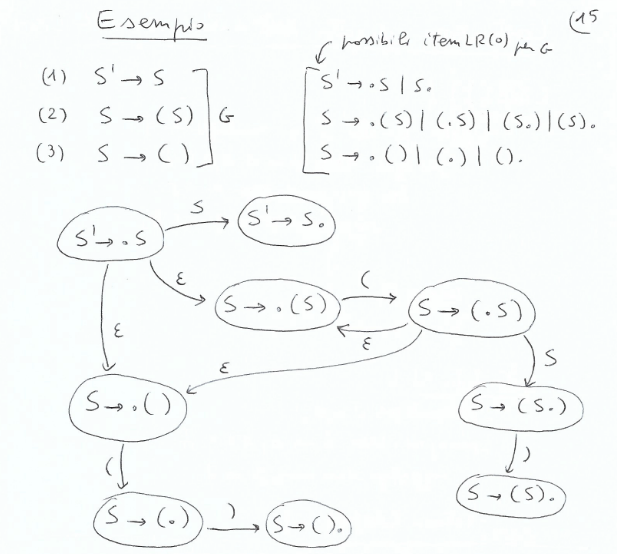
\includegraphics[width=0.7\textwidth]{img/esempio64.png}
\end{center}
\vspace{1em} 
\subsection{Automa canonico LR(o)}
\begin{itemize}
  \item È il DFA che si ottiene dall'NFA dei prefissi viabili mediante la costruizione per sottoinsiemi 
  \begin{center}
    oppure
  \end{center}
  \item In un modo diretto usando le funzioni ausiliarie 
  \begin{align*}
    Clos(I) \quad Goto(I, x)
  \end{align*}
  dove $I$ è un insieme di item e $x \in T \cup NT$
\end{itemize}
\subsection{Costruizione diretta dell'automa canonico LR(o)}
\begin{itemize}
  \item $Clos(I)$
  \begin{itemize}
    \item ripeti finchè $I$ è modificato
    \begin{itemize}
      \item per ogni item $A \to \zeta . xB \in I$
      \begin{itemize}
        \item per ogni produzione $x \to y$ \\
        $\quad \quad $- aggiungi $x \to .y$ ad $I$;
      \end{itemize}
    \end{itemize}
    \item return I
  \end{itemize}
\end{itemize}
\begin{itemize}
  \item $Goto(I, X)$
  \begin{itemize}
    \item inizializza $j = \emptyset$
    \item per ogni item $A \to \zeta . xB \in I$
    \begin{itemize}
      \item aggiungi $A \to \zeta x.B$ a $J$
    \end{itemize}
    \item return $Clos(j)$
  \end{itemize}
\end{itemize}
\vspace{1em}
\begin{itemize}
  \item Inizializza $S' = \{Clos(\{S' \to S\})\}$;
  \item Inizializza $\delta = \emptyset$;
  \item Ripeti finchè $S'$ o $\delta$ vengano modificati
  \begin{itemize}
    \item per ogni $I \in S'$
    \begin{itemize}
      \item per ogni item $A \to \zeta .x B \in I$
      \begin{itemize}
        \item sia $j = Goto(I,x)$;
        \item aggiungi $J$ a $S'$;
        \item aggiungi $\delta(I, x) = j$ a $\delta$;
      \end{itemize}
    \end{itemize}
  \end{itemize}
  \item return $S'$ e $\delta$
\end{itemize}
  \begin{center}
    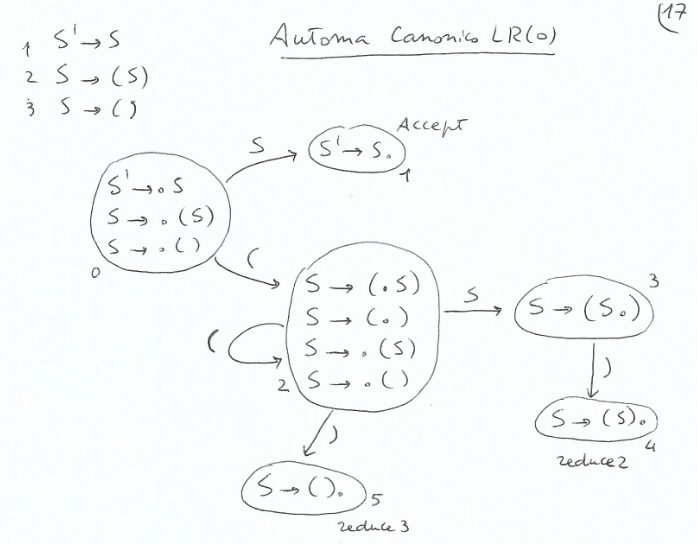
\includegraphics[width=0.7\textwidth]{img/esempio65.png}
\end{center}
  \begin{center}
    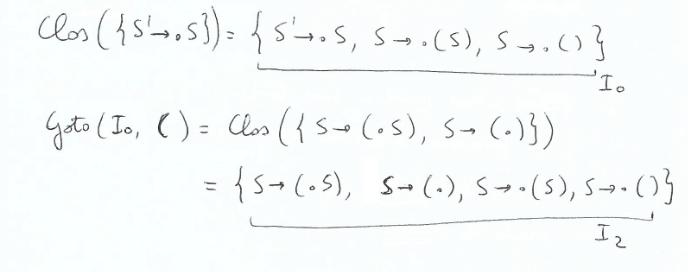
\includegraphics[width=0.7\textwidth]{img/esempio66.png}
\end{center}
\subsection{Tabella di parsing LR}
\begin{itemize}
  \item Matrice bidimensionale $M$
  \begin{itemize}
    \item righe= stati dell'automa canonico LR(o)/LR(1)
    \item colonne= $\underbrace{T \cup \{\mathdollar\}}_\text{azione} \cup \underbrace{NT}_\text{goto}$ 
  \end{itemize}
  \item $M[S,x]$ contiene le azioni che può compiere un parser LR con $S$ in cima alla pila degli stati e $x$ simbolo in input (o nonterminale)
  \item Se $M[S, x]$ è "bianca" / vuota allora ERRORE
  \item Se $M[S,x]$ contiene più azioni allora CONFLITTO (il parser non è deterministico)
\end{itemize} 
\vspace{1em}
\textit{Caso}: LR(o) \\
Per ogni stato $S$ dell'automa canonico LR(o)
\begin{itemize}
  \item se $x \in T$ e $S \to^X t$ nell'automa LR(o) inserisci shift in $M[s, x]$
  \item se $A \to \zeta . \in s$ e $A \neq S'$ inserisci reduce $A \to \zeta$ in $M[s,x]$ per tutti gli $x \in T \cup \{\mathdollar\}$
  \item se $S' \to S . \in s$ e $A \neq S'$ inserisci reduce $A \to \zeta$ in $M[s,x]$ per tutti gli $x \in T \cup \{\mathdollar\}$
  \item se $A \in NT$ e $s \to^A t$ nell'automa LR(o), inserisci goto t in $M[s,A]$
\end{itemize}
\textit{Definizione}: Una grammatica è di classe LR(o) se ogni casella nella tabella di parsing LR(o) contiene al più un elemento!
  \begin{center}
    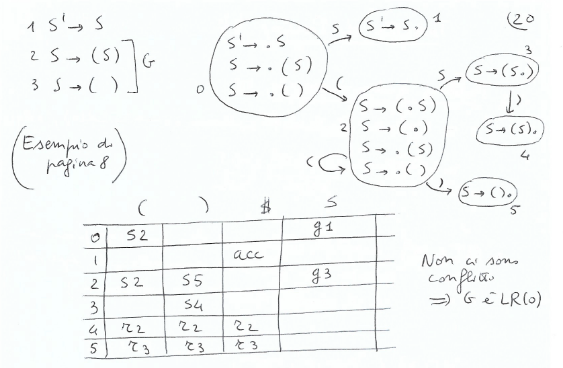
\includegraphics[width=0.7\textwidth]{img/esempio67.png}
\end{center}
  \begin{center}
    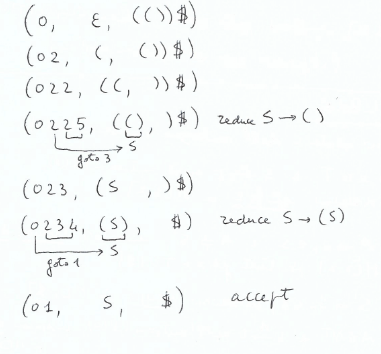
\includegraphics[width=0.5\textwidth]{img/esempio68.png}
\end{center}
\subsection{Il generico Parser LR}
(con solo lo stack degli stati) 
\begin{itemize}
  \item Inizializza la pila con $\mathdollar S_0$; %in cima alla pila a dx $S_0$ stato iniziale dell'automa
  \item Inizializza $i_c$ con il primo carattere in input;
  \item while(true)
  \begin{itemize}
    \item S = top(pila); %top non rimuove la testa
    \item case $M[s, i_c]$ of
      \begin{itemize}
        \item shift: {push sulla pila; avanza $i_c$ sull'input;}
        \item accept: {output('accept'); break;}
        \item reduce $A \to \zeta$: 
          \begin{itemize}
            \item pop $\mid \zeta \mid$ stati della pila;
            \item $s_1 = $ top(pila); %$s_1$ contiene $B \to y . A \delta$
            \item Sia $s_2 = M[s_1, A]$; % $M[s_1, A]$ è goto $s_2$
            \item push $s_2$ sulla pila
            \item output la produzione $A \to \zeta$;
          \end{itemize}
        \item $errore()$;
      \end{itemize}
  \end{itemize}
\end{itemize}
\vspace{1em}
\subsection*{Non sempre siamo cosi' fortunati $\dots$}
Una grammatica libera $G$ puo' non essere LR(o)!
\begin{align*}
  \text{(1) } S' \to S \quad \text{ (2) } S \to a \text{ (3) } S \to ab \quad \quad L(G)=\{a, ab\}
\end{align*}
  \begin{center}
    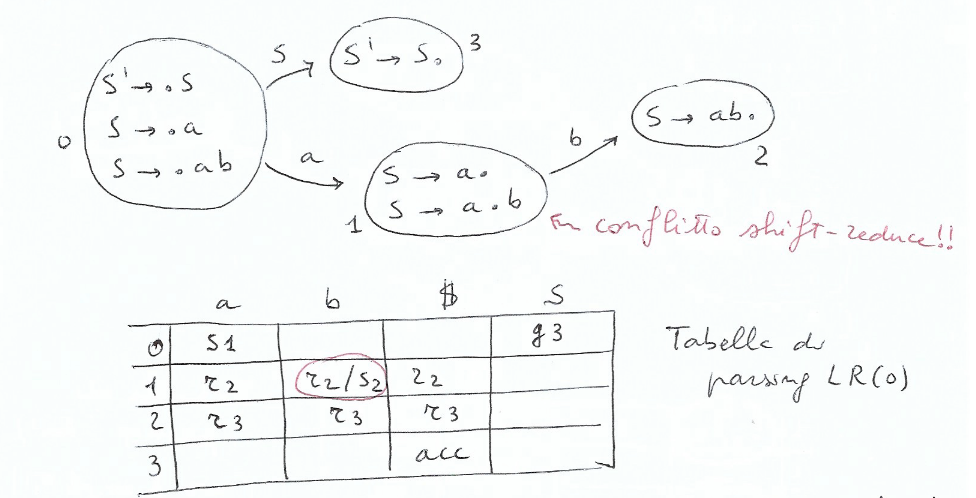
\includegraphics[width=0.7\textwidth]{img/esempio69.png}
\end{center}
Come risolvere il conflitto? Usiamo il look-ahead! Cioe' guardiamo il $Follow(S)$: se $b \in Follow(S)$, allora il conflitto puo' essere reale! Altrimenti no! \\
\begin{center}
  Ma $Follow(S) = \{\mathdollar\} \to $ risolviamo il conflitto a favore dello shift 
\end{center}
  \begin{center}
    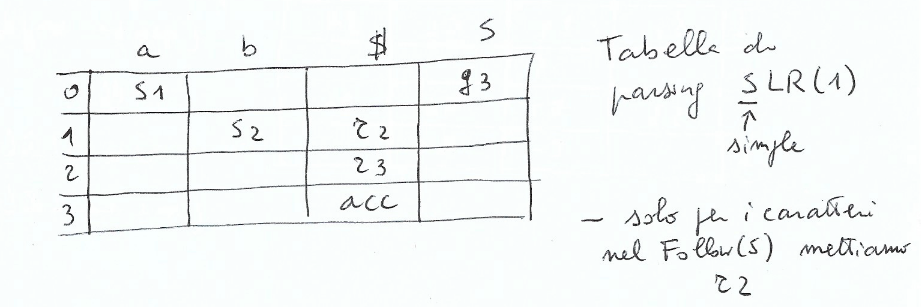
\includegraphics[width=0.7\textwidth]{img/esempio70.png}
\end{center}
\vspace{1em} 
\textit{Esempio}: Parentesi bilanciate
\begin{align*}
  \text{(0) } S' \to S \quad \text{ (1) } S \to (S)S \quad \text{ (2) } S \to \epsilon
\end{align*}
  \begin{center}
    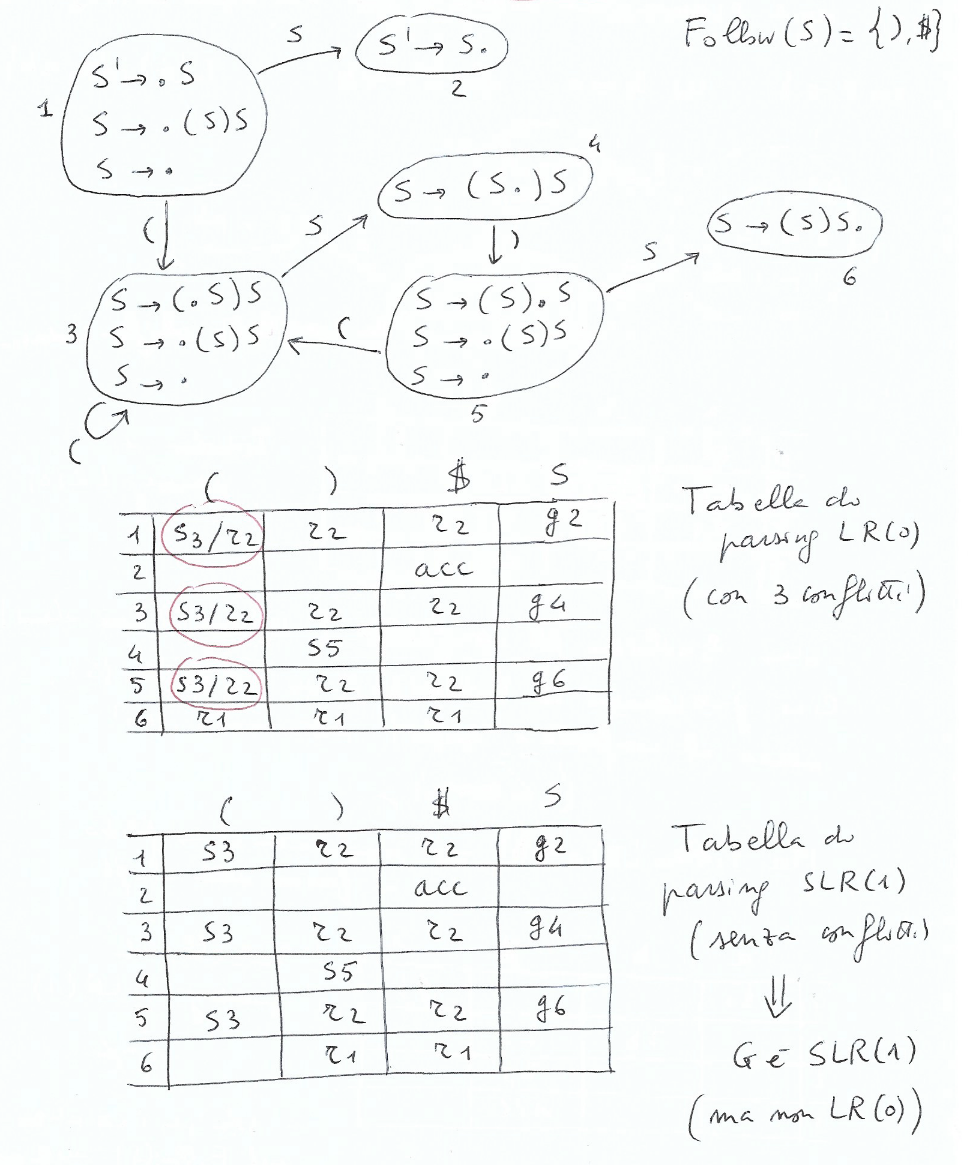
\includegraphics[width=0.7\textwidth]{img/esempio71.png}
\end{center}
\textit{Osservazioni}:
\begin{itemize}
  \item Se $G$ ha produzioni $\epsilon$, allora $G$ difficilmente e' LR(o)
  \item Se $L$ e' libero deterministico e gode della prefix-propriety allora $L$ e' LR(o). Quindi se $L$ e' libero deterministico ma non e' LR(o) allora $L$ non gode della prefix-propriety.
  \item Se $L$ e' LR(o) ed e' finito, allora gode della prefix-propriety. Ovvero se $L$ e' finito e non gode della prefix-propriety allora $L$ non e' LR(o)
  \item Se $L$ e' LR(o) ma e' infinito puo' non godere della prefix-propriety
\end{itemize}
  \begin{center}
    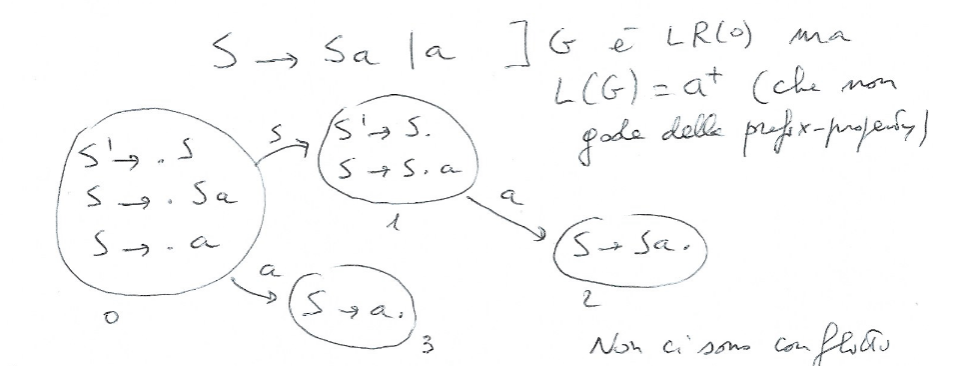
\includegraphics[width=0.7\textwidth]{img/esempio72.png}
\end{center}
\section{Tabella di Parsing SLR(1)}
\begin{align*}
  \underbrace{\text{S}}_\text{simple}\text{LR(1)}
\end{align*}
\begin{itemize}
  \item colonne: $T \cup \{mathdollar\} \cup NT$
  \item righe: stati dell'automa canonico LR(o)
\end{itemize}
Come si riempe la tabella? \\\
Per ogni stato $s$ dell'automa LR(o)
\begin{itemize}
  \item se $x \in T$ e $s \to^x t$ inserisci \textit{shift t} in $M[s,x]$
  \item se $A \to \zeta. \in s$ e $A \neq S'$ inserisci \textit{reduce $A \to \zeta$} in $M[s,x]$ per tutti gli $x \in Follow(A)$ (\textit{nota}: prima per LR(o) era "per tutti gli $x \in T \cup \{\mathdollar\}$", questo serve per limitare l'uso della reduce solo a casi plausibili!)
  \item se $S' \to S. \in s$ inserisci \textit{accept} in $M[s,\mathdollar]$
  \item se $A \in NT$ e $S \to^A t$ inserisci \textit{goto t} in $M[s,A]$
\end{itemize}
SLR(1):
\begin{itemize}
  \item S: simple
  \item L: left-to-right
  \item R: rightmost derivation
  \item 1: un simbolo di look-ahead (attraverso i follow dei nonterminali)
\end{itemize}
Vedremo che LR(1) usa esplicitamente il look-ahead gia' nella definizione di \textit{item} LR(1) \\
\vspace{1em} \\
\subsection*{Ma non siamo sempre cosi' fortunati $\dots$ di nuovo!}
Una grammatica libera $G$ potrebbe non essere nemmeno SLR(1)!
\begin{align*}
  \text{(0) } S' \to S \quad \text{ (1) } S \to V = E \quad \text{ (2) } S \to E \quad \text{ (3) } E \to V \quad \text{ (4) } V \to x \quad \text{ (5) } V \to *E
\end{align*}
  \begin{center}
    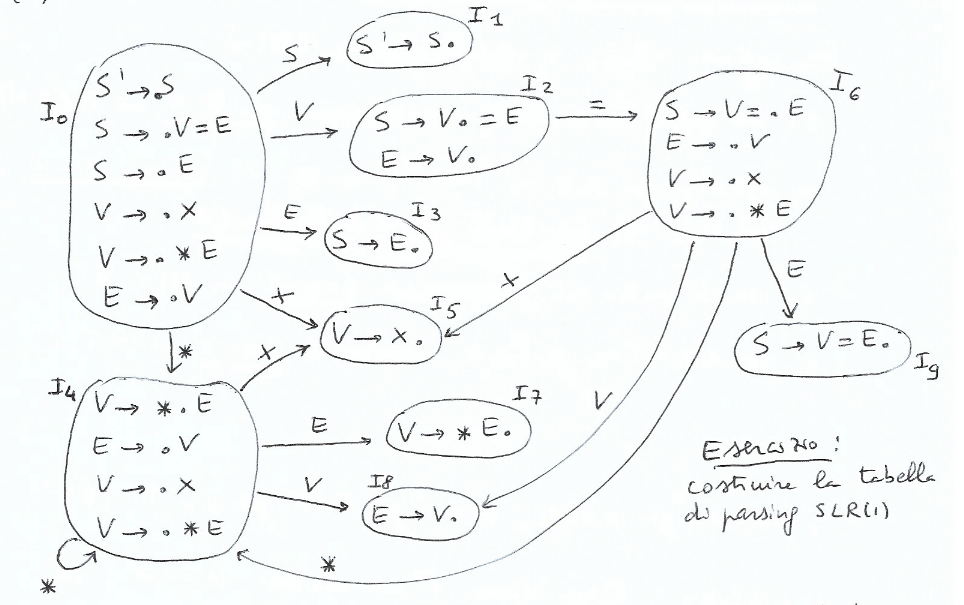
\includegraphics[width=0.7\textwidth]{img/esempio73.png}
\end{center}
Consideriamo: $I_2$
\begin{align*}
  S \to V. = E \\
  E \to V.
\end{align*}
conflitto shift/reduce perche' $+ \in Follow(E)$ (a causa di $V \to *E$ si ha $Follow(V) \subseteq Follow(E)$) \\
$M[I_2, =] = \{s_6, r_3\}$ nella tabella di parsing SLR(1) \\
\textit{Osservazione}: Se noi sappiamo con certezza che il carattere successivo e' davvero "\textit{=}" allora la reduce $E \to V.$ non va considerata perche' non e' mai possibile derivare
\begin{align*}
  S \to^* E = \dots
\end{align*}
$\to$ ha senso solo fare la shift! \\
\vspace{5px} \\
\textit{Osservazione}: $\quad = \in Follow(E)$ vuol dire che esiste una derivazione tale che $S \to^* \zeta E = B$ ma a noi serve sapere se
\begin{align*}
  S \to^* E = B
\end{align*}
perche' questa e' la derivazione "\textit{corrente}".  \\\
\vspace{1em} \\
\textit{Nota bene}: 
\begin{align*}
  S \to V = E \to *E = E
\end{align*}
per cui effettivamente $= \in Follow(E)$ ma e' impossibile derivare 
\begin{align*}
  S \to^* E = \dots
\end{align*}
per cui nello stato $I_2$ se in input c'e' $=$ devo sicuramente fare lo shift a $I_6$. \\
\vspace{1em} \\
Da questo esempio si capisce che bisogna ridurre i casi in cui si possa applciare una "reduce" a casi ancora piu' plausibili di quantop dica il $Follow(E)$! \\
$\to$ \textit{item LR(1)}: una coppia formata da 
\begin{itemize}
  \item un item LR(o) (detto nucleo 0 core)
  \item un simbolo di look-ahead in $T \cup \{\mathdollar\}$
\end{itemize}
\textit{Esempio}: $I_2$
\begin{align*}
  [S \to V. = E, \mathdollar] \\
  [E \to V., \mathdollar]
\end{align*}
\begin{itemize}
  \item stato dell'automa canonico LR(1)
  \item se leggo $=$ allora shift
  \item se leggo $\mathdollar$ allora reduce $E \to V$
\end{itemize}
\vspace{1em} 
\textit{Introduzione}: se l'automa canonico LR(1) e' in uno stao che contiente l'item LR(1) $[A \to \zeta . B , x]$
\begin{itemize}
  \item sta cercando di riconoscere la maniglia $\zeta B$;
  \item di essa $\zeta$ e' gia' sulla pila;
  \item sull'input si aspetta una stringa derivabile da $Bx$ (cioe' $x$ puo' essere fatta in questa derivazione)
  \item $[A \to \zeta. , x] \quad $ $\to$ fai la reduce $A \to \zeta$ se il prossimo input e' proprio $x$ 
\end{itemize}
\textbf{Item LR(1)} usiamo esplicitamente 1 carattere in avanti dell'input associato direttamente all'item LR(o)-core. \\
\vspace{1em} \\
\subsection{NFA LR(1)}
\begin{itemize}
  \item stati: item LR(1) della grammatica aumentata 
  \item $[S' \to .S, \mathdollar]$ e' lo stato iniziale
  \item dallo stato $[A \to \zeta . xB, a]$ c'e' una transizione allo stato $[A \to \zeta x . B, a]$ etichettata $x$ per $x \in T \cup NT$
  \item dallo stato $[A \to \zeta . xB, a]$ per $x \in NT$ e per ogni produzione $x \to \gamma$ c'e' una $\epsilon$-transizione verso lo stato $[x \to .y, b]$ per ogni $b \in First(Ba)$ (\textit{Nota bene}: $First(Ba) \subseteq T \cup \{\mathdollar\}$)
\end{itemize}
\vspace{1em}
\subsection{Automa canonico LR(1)}
Si puo' ottenere in 2 modi:
\begin{itemize}
  \item DFA ottenuto da NFA LR(1) con la costuizione dei sottoinsiemi
  \item In modo diretto usando le funzioni $Clos(I)$ e $Goto(I,x)$ partendo dallo stato iniziale $Clos([S' \to .S, \mathdollar])$
\end{itemize}
\vspace{5px}
\begin{itemize}
  \item $Clos(I)$
  \begin{itemize}
    \item ripeti finché $I$ è modificato
    \begin{itemize}
      \item per ogni item $[A \to \zeta . xB,a] \in I$
      \begin{itemize}
        \item per ogni produzione $x \to y$
        \begin{itemize}
          \item per ogni $b \in First(Ba)$
          \begin{itemize}
            \item aggiungi $[x \to .y, b]$ a $I$;
          \end{itemize}
        \end{itemize}
      \end{itemize}
      \item return $I$;
    \end{itemize}
  \end{itemize}
\end{itemize}
\vspace{1em}
\begin{itemize}
  \item $Goto(I,x)$
  \begin{itemize}
    \item inizializza $J = \emptyset$
    \item per ogni item $[A \to \zeta . xB, a] \in I$
    \begin{itemize}
      \item aggiungi $[A \to \zeta x . B, a]$ a $J$
    \end{itemize}
    \item return $Clos(J)$
  \end{itemize}
\end{itemize}
Stato iniziale dell'automa canonico LR(1) e' $Clos([S' \to .S, \mathdollar])$ \\
\textit{Osservazione}: $Goto(I,x)$ non considera il look-ahead cioe' agisce solo sulla parte "\textit{core / LR(o)}" dell'item LR(1) (salto poi effetturare $Clos(J)$ in chiusura) \\
\vspace{2em} \\
\begin{align*}
  \text{(o) } S' \to S \quad \text{ (1) } S \to CC \quad \text{ (2) } C \to cC \quad \text{ (3) } C \to d
\end{align*}
  \begin{center}
    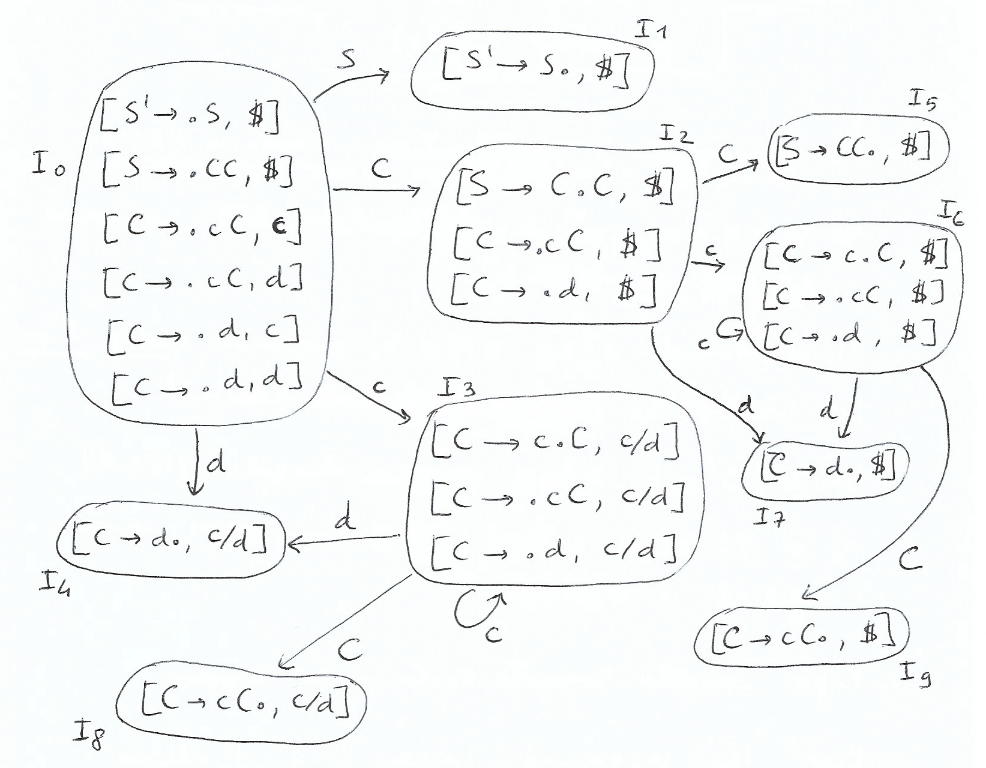
\includegraphics[width=0.7\textwidth]{img/esempio74.png}
\end{center}
\vspace{1em}
\subsection{Come si deve riempire la tabella di parsing LR(1)?}
Per ogni stato $s$ dell'automa canonico LR(1)
\begin{itemize}
  \item se $x \in T$ e $s \to^x t$ nell'automa LR(1) inserisci \textit{shift t} in $M[s,x]$
  \item se $[A \to \zeta . , x] \in s$ e $A \neq S'$ inserisci \textit{reduce $A \to \zeta$} in $M[s,x]$ (solo per $x$ del look-ahead!)
  \item se $[S' \to S . , \mathdollar] \in s$ inserisci \textit{Accept} in $M[s, \mathdollar]$
  \item se $A \in NT$ e $s \to^A t$ nell'automa LR(1) inserisci \textit{goto t} in $M[s,A]$
\end{itemize}
Ogni casella rimasta vuota e' un errore! \\
\textit{Deinizione}: Una grammatica libera $G$ e' di classe LR(1) se ogni casella della sua tabella di parsing LR(1) ha al piu' un elemento (no conflitti)
  \begin{center}
    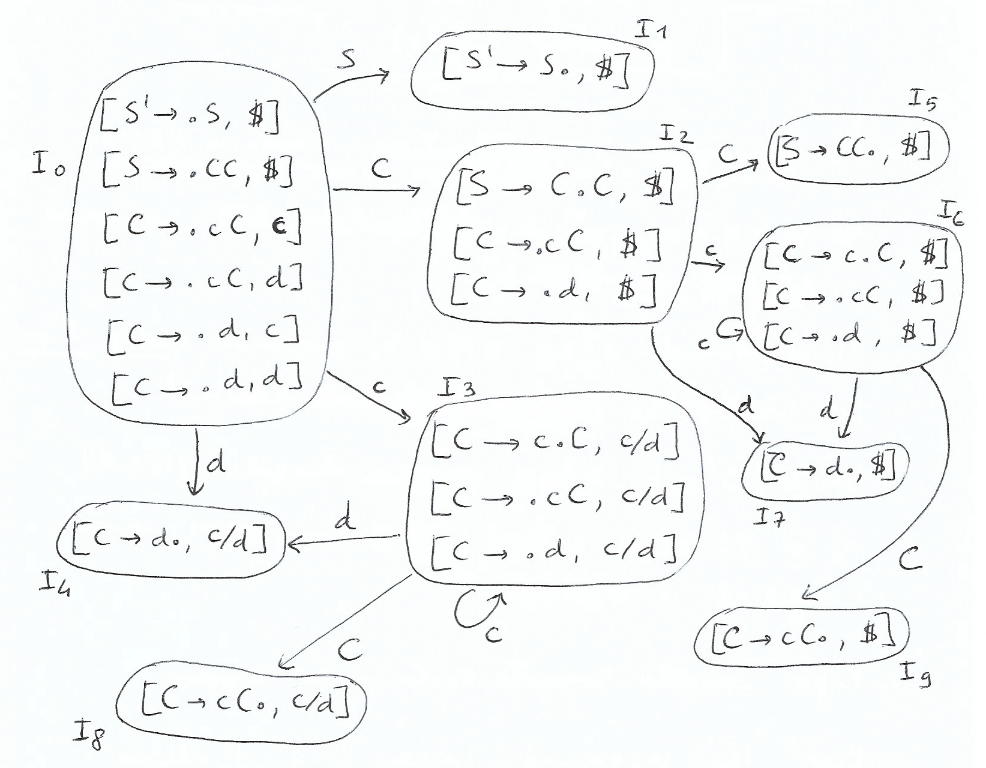
\includegraphics[width=0.7\textwidth]{img/esempio74.png}
\end{center}
\begin{itemize}
  \item La tabella SLR(1) per questa grammatica ha solo 7 stati anziche' 1, ed e' pure senza conflitti!
  \item Vedremo che questa grammatica e' (ovviamente) anche LALR(1)
\end{itemize} 
\vspace{1em}
Riconsideriamo la grammatica \textbf{NON SLR(1)}
\begin{align*}
  \text{(0) } S' \to S \quad \text{ (1) } S \to V = E \quad \text{ (2) } S \to E \quad \text{ (3) } E \to V \quad \text{ (4) } V \to x \quad \text{ (5) } V \to *E
\end{align*}
e vediamo se e' LR(1)!
  \begin{center}
    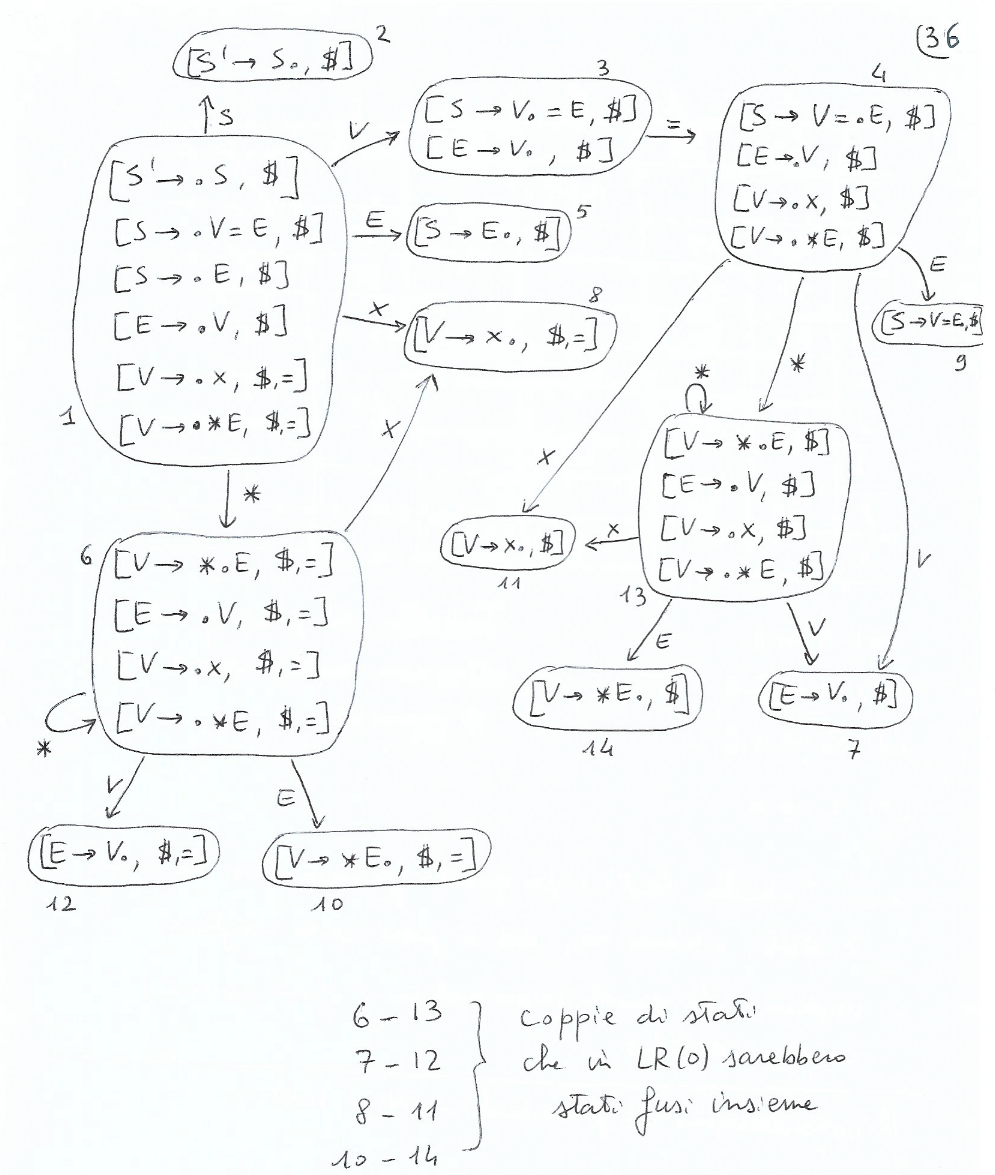
\includegraphics[width=0.7\textwidth]{img/esempio76.png}
\end{center}
\begin{center}
  \textbf{Tabella di parsing LR(1)}
\end{center}
  \begin{center}
    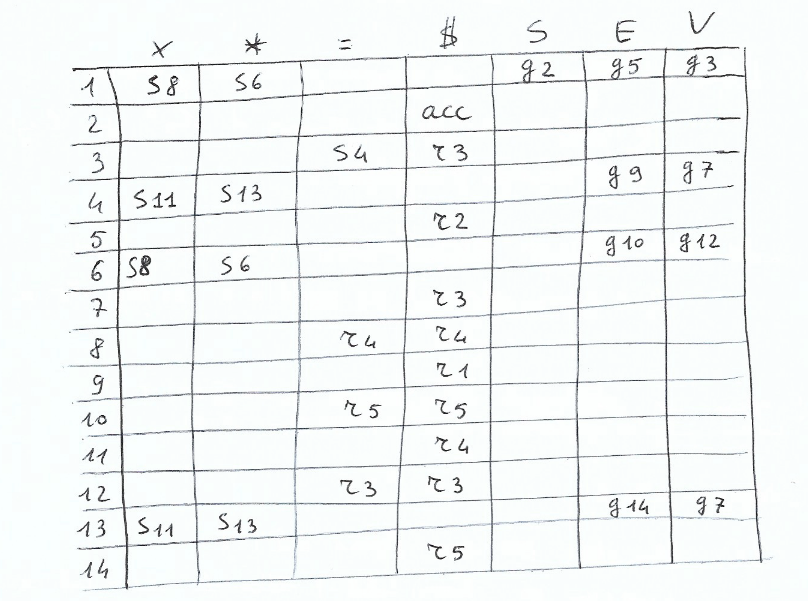
\includegraphics[width=0.7\textwidth]{img/esempio77.png}
\end{center}
\begin{align*}
  \text{(0) } S' \to S \quad \text{ (1) } S \to V = E \quad \text{ (2) } S \to E \quad \text{ (3) } E \to V \quad \text{ (4) } V \to x \quad \text{ (5) } V \to *E
\end{align*}
Non ci sono conflitti! $\quad \to G$ e' LR(1)! \\
\vspace{1em} \\
\subsection{Parser LALR(1)} 
\begin{align*}
  \text{Parser } \underbrace{\text{LA}}_\text{look-ahead} \text{LR(1)}
\end{align*}
\begin{itemize}
  \item LR(1): tabelle di parsing molto grandi (centinaia di migliaia)
  \item LALR(1): buon compromesso tra semplicita (e compatezza) di SLR(1) e selettivita' di LR(1)
\end{itemize}
\vspace{1em}
\subsection{Come si ottiene il parser LALR(1)?}
Osserva che: 
\begin{itemize}
  \item Nucleo di uno stato LR(1):
  \begin{itemize}
    \item insieme di item LR(o) ottenuto dimenticando i look-ahead degli item LR(1)
  \end{itemize}
  \item Nucleo di stato LR(1) = stato dell'automa LR(o)
  \item Le transizioni dell'automa LR(1) dipendono solo dal nucleo
  \begin{itemize}
    \item la funziona $Goto(I, x)$ usa $I$ solo la parte "\textit{nucleo}"\textit{/LR(o)} dell'item LR(1)
  \end{itemize}
\end{itemize}
$\to$ La tabella di parsing LALR(1) si ottiene da quella LR(1) fondendo insieme gli stati con lo stesso nucleo
\begin{itemize}
  \item tante righe quanti gli stati dell'automa LR(o)
  \item meno "reduce" della tabella SLR(1)
\end{itemize}
Riprendiamo l'esempio delle scorse pagine:
  \begin{center}
    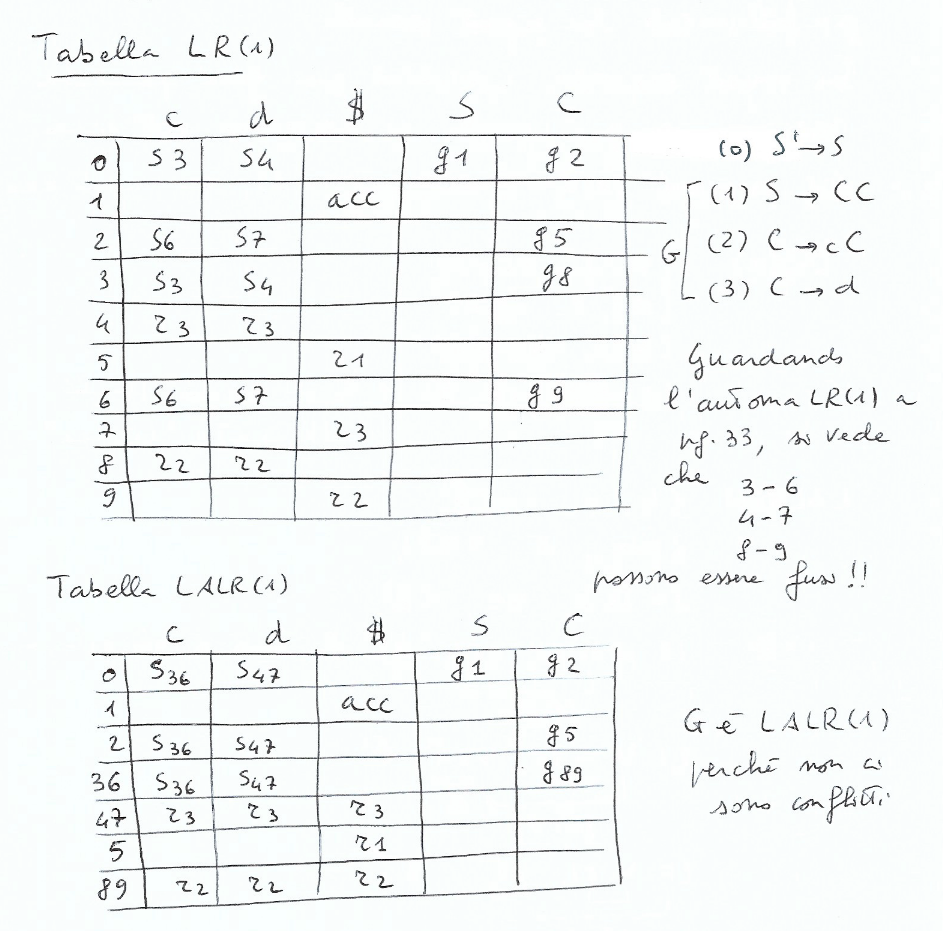
\includegraphics[width=0.7\textwidth]{img/esempio78.png}
\end{center}
\begin{align*}
  I_{36} = I_3 \cup I_6 = \{[c \to c . C, c/d/\mathdollar] , \\
  [c \to .cC, c/d/\mathdollar], \\
  [c \to .d , c/d/\mathdollar]\}
\end{align*}
Se $G$ e' LR(1) e anche LALR(1) allora l'automa LR(1) e quello LALR(1) si mimano perfettamento su input corretti. Su input erronei LALR(1) puo' fare qualche riduzione in piu' prima di accorgersi dell'errore. Ad esempio per la $G$ (esempio precedente) su input $ccd\mathdollar$
  \begin{center}
    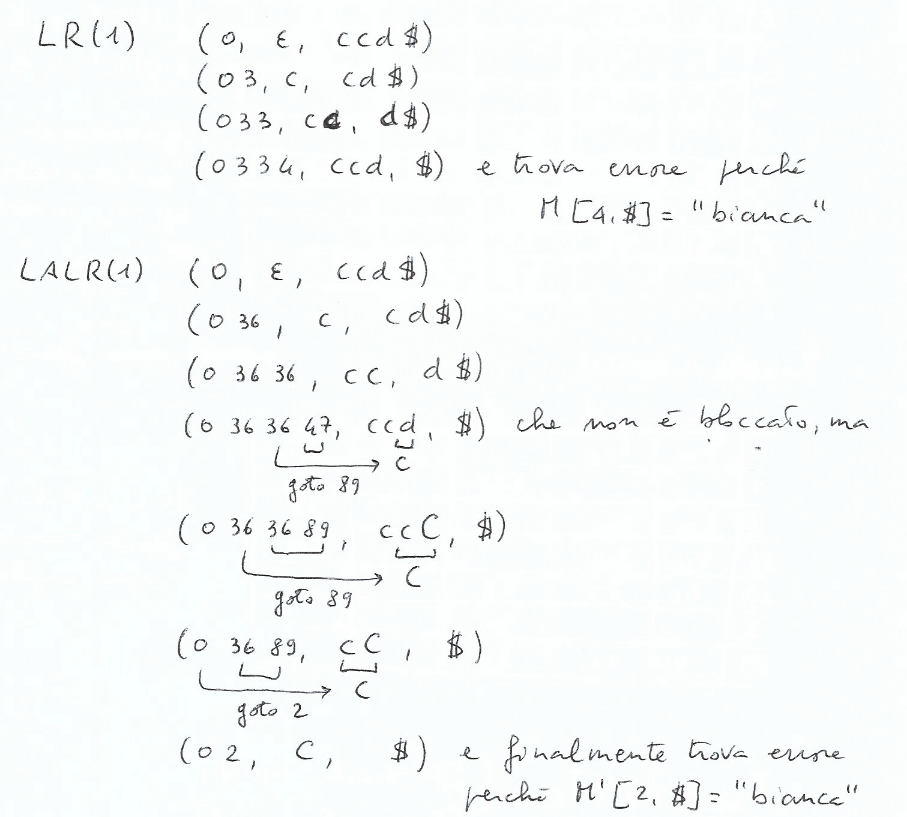
\includegraphics[width=0.7\textwidth]{img/esempio79.png}
\end{center}
L'automa LALR(1) non fara' mai degli shift in piu' dell'automa LR(1) per un certo input. 
\begin{itemize}
  \item $\to$ i due parser consumano la stessa porzione di input prima di rilevare l'errore
  \item $\to$ LALR(1) e' corretto come sostituto di LR(1)
\end{itemize}
Riprendiamo l'esempio precedente
  \begin{center}
    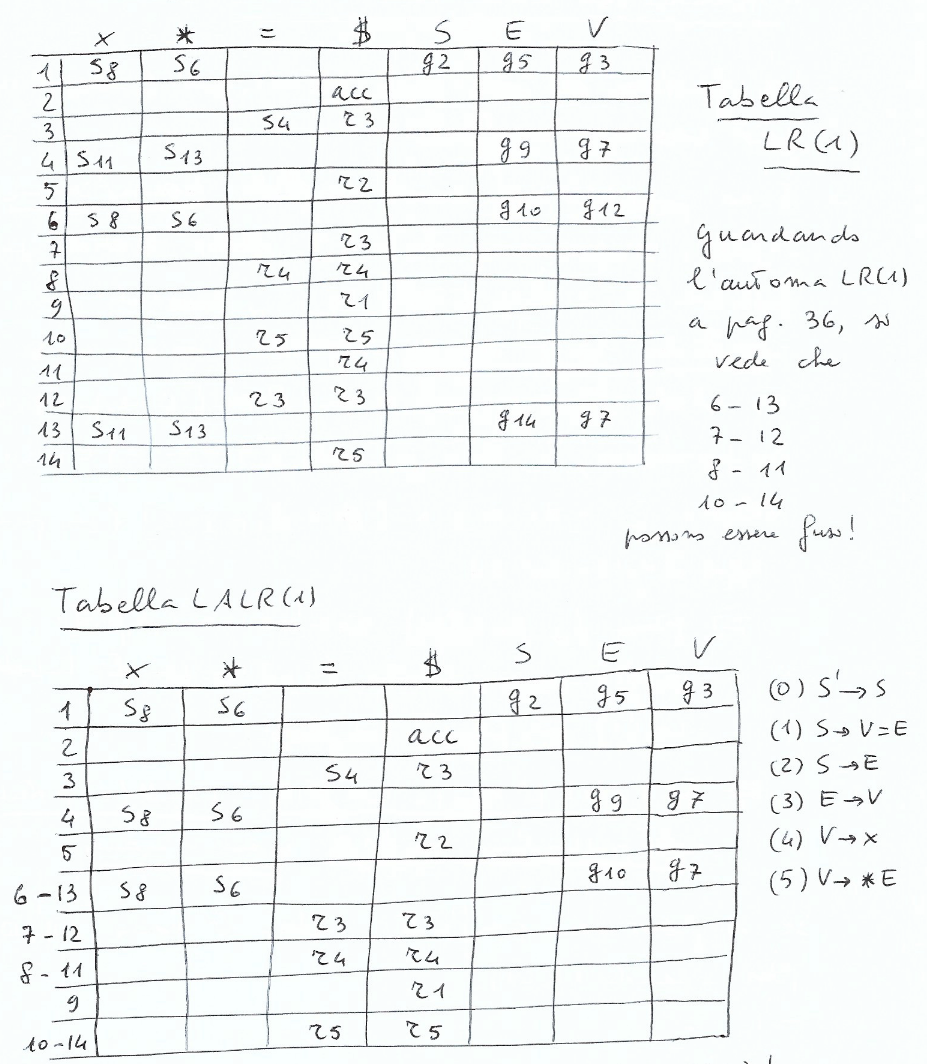
\includegraphics[width=0.7\textwidth]{img/esempio80.png}
\end{center}
\begin{center}
  Non ci sono conflitti $\to$ $G$ e' LALR(1)!
\end{center}
Tabella grande come quelle SLR(1) per $G$ ma questa non ha conflitti!!! \\
\vspace{1em}\\
\subsection{Passando da LR(1) a LALR(1)}
\begin{itemize}
  \item La fusione di due stati LR(1) con lo stesso core puo' causare conflitti
  \item Sono possibili solo nuovi conflitti \textit{reduce/reduce}. Infatti supponiamo che in $s$ stato ottenuto per fusione di 2 stati LR(1) $s_1$ e $s_2$ presenti un \textit{conflitto shift-reduce}. Allora esiste in $s$ un item $[A \to \zeta., a]$ e un item $[B \to \beta . a \gamma, b]$. Supponiamo $w.l.o.g.$, che $[A \to \zeta . , a] \in s_1$. Allora $[A \to \zeta . , a]$ e $[B \to \beta . a \gamma , c]$ (per qualche $c$) appartengono ad $s_1$!
  \begin{itemize}
    \item $\to$ pure $s_1$ in LR(1) avrebbe un conflitto shift-reduce, contro l'ipotesi che la tabella LR(1) non presenti conflitti!
    \item $\to$ Se LR(1) e' senza conflitti, LALR(1) potrebbe solo presentare conflitti \textit{reduce-reduce}
  \end{itemize}
\end{itemize}
Se si generano conflitti allora $G$ non e' LALR(1) pur essendo LR(1).
  \begin{center}
    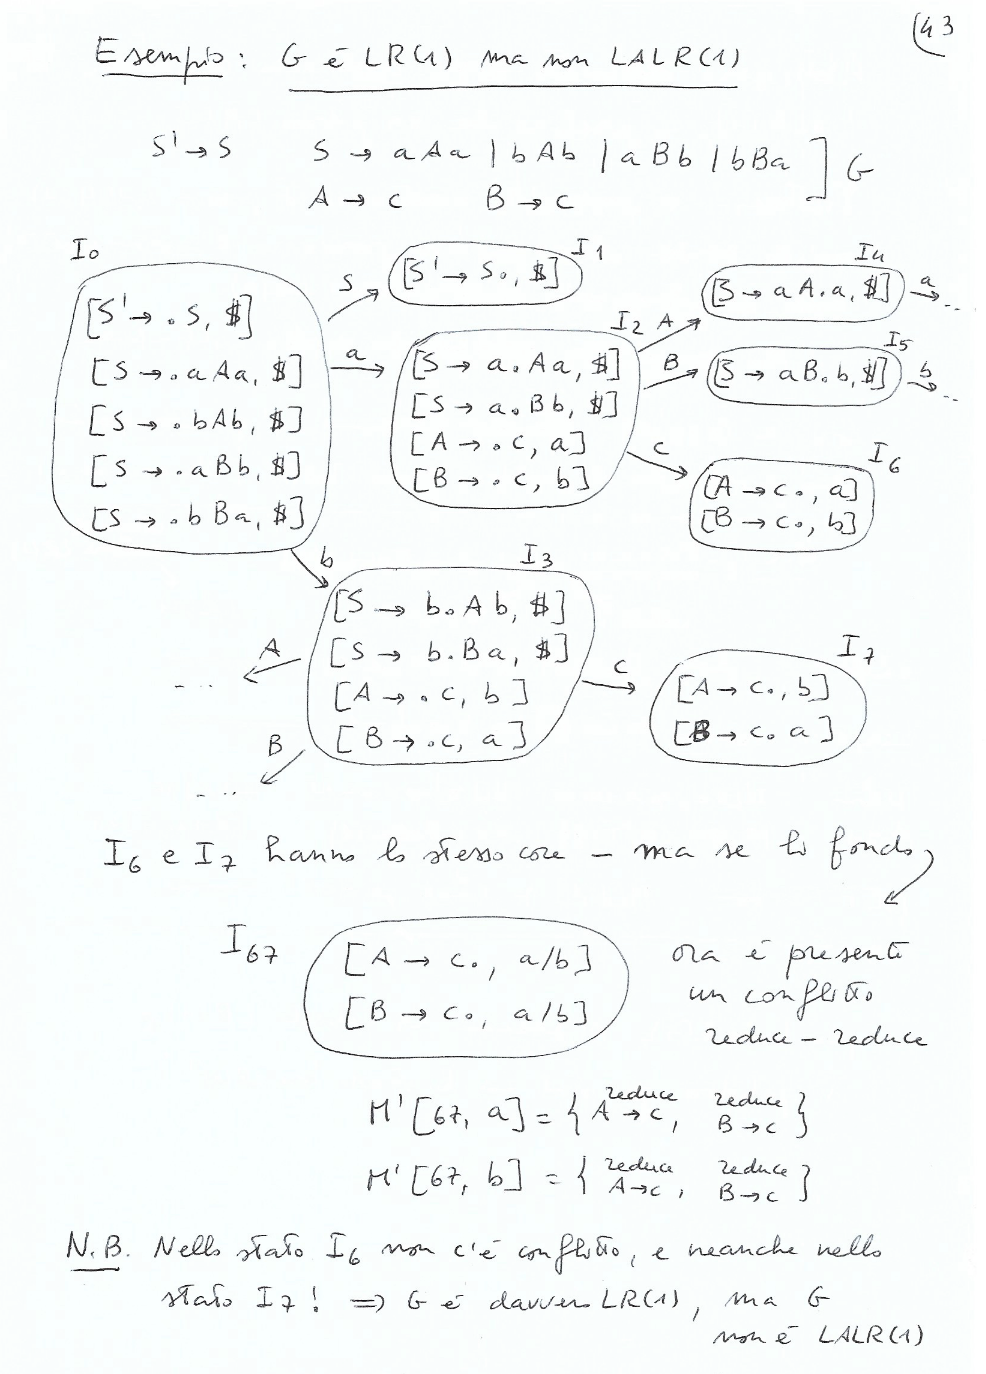
\includegraphics[width=0.9\textwidth]{img/esempio81.png}
\end{center}
\vspace{1em}
Abbiamo descritto come costuire un parser LALR(1) a partire da un parser LR(1). Tuttavia e' possibili costruire il parser LALR(1) anche senza dover prima generare l'automa LR(1), ma direttamente dall'automa LR(o).
\begin{center}
  $\to$ maggiore efficienza nella costuizione
\end{center}
Questa tecnica (che non vedremo) e' quella usata dai generatori di parser, quali \textit{yacc} (che vedremo).  \\
\vspace{1em}\\
\textbf{Ricapitolando}
  \begin{center}
    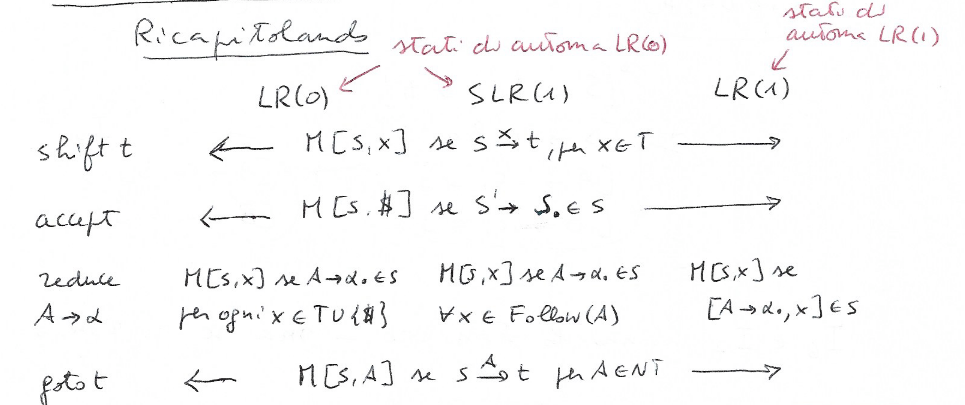
\includegraphics[width=0.7\textwidth]{img/esempio82.png}
\end{center}
per LALR(1) si prende la tabella LR(1) e si fondono gli stati con lo stesso "core LR(o)". \\
\vspace{1em} \\
\section{Grammatiche LR(k)}
\begin{itemize}
  \item item LR(k) $= [\text{item LR(o), B}]$ con $\mid B \mid \leq k$
  \item item iniziale $= [S' \to .S, \mathdollar]$
  \item Quando $[A \to \zeta . x \gamma, B] \in s$ (stato dell'automa canonico KR(k)) allora pure $[x \to . \delta, w] \in s$ se $x \to \delta$ e' una produzione e $w \in First_k(\gamma B)$
  \item Tabella con colonne su $T \cup \mathdollar$ (per shift e accept), piu' tutti i $w$ tali che esiste un item $[A \to \zeta . , w]$ (per le reduce)
  \item Affinche' $G$ sia LR(k) bissogna che la tabella di parsing LR(k) ottenuta a partire dall'automa canonico LR(k)
  \begin{itemize}
    \item contenga al piu' una aazione per ogni entrata della tabella
    \item non esistano due $w_1$ e $w_2$ sulle colonne tali che $w_1$ e' prefisso di $w_2$ e per almeno una riga le 2 corrispondenti entrate contengano un'azione
  \end{itemize}
\end{itemize}
\vspace{1em}
\subsection{Grammatiche SLR(k)}
Si parte dall'automa canonico LR(o) e si riempe la tabella di parsing SLR(k) cje ja colonne su $T \cup \mathdollar$ (per shift/accept) e in piu' sui $w \in Follow_k (A)$ per $A \to \zeta .$ seconda la legge
\begin{itemize}
  \item se $[A \to \zeta.] \in s$ e $A \neq S'$ inserisci "reduce $A \to \zeta$" in $M[s, w]$ per tutti i $w \in Follow_k (A)$
\end{itemize}
Se la tabella di parsing SLR(k) cosi' riempita non ha conflitti (e se non esistono $w_1$ e $w_2$ sulle colonne tali che $w_1$ su prefisso di $w_2$ con una riga su cui le 2 entrate sono entrambe riempiti), allora $G$ e' SLR(k). \\
\vspace{1em} \\
\subsection{Grammatiche LALR(k)}
Si parte dell'automa canonico LR(k) e si fondono insieme gli stati con lo stesso nucleo. Se la tabella risultante non presenta conflitti (e in piu' non esistono $w_1$ e $w_2$ tali che $\dots$) allora $G$ e' LALR(k).
\begin{center}
  \textbf{Relazione tra grammatiche LL(k) e LR(k)}  
\end{center}
  \begin{center}
    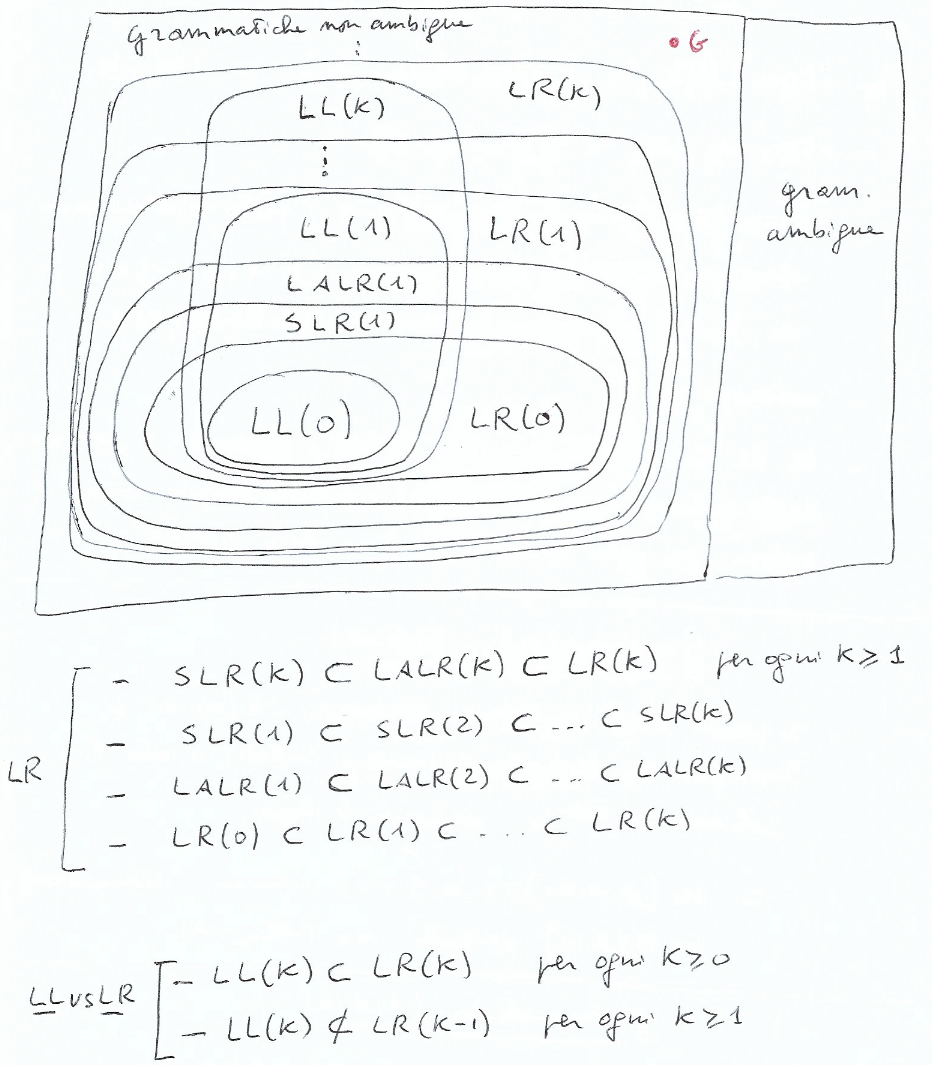
\includegraphics[width=0.9\textwidth]{img/esempio83.png}
\end{center}
\vspace{1em}
Proposizione
\begin{itemize}
  \item Se $G$ e' LL(k) allora $G$ e' non ambigua e L(G) e' deterministico
  \item Se $G$ e' LR(k) allora $G$ e' non ambigua e L(G) e' deterministico
\end{itemize}
\textit{Osservazione}: Esistono linguaggi generati da grammatiche non ambigue, ma nondeterministici
\begin{align*}
  S \to aSa \mid bSb \mid \epsilon ] G \\
  L(G) = \{ww^R \mid w \in \{a,b^*\}\}
\end{align*}
\vspace{1em} 
\subsection*{Ma cosa possiamo dire dei linguaggi generati da tali grammatiche?}
\textit{Definizione}: Un linguaggi L e' di classe $X$ se $\exists G$ di classe $X$ tale che $L = L(G)$. (dove $X$ sta per LR(o)/SLR(1)/LL(1)/$\dots$) \\
Se classifichiamo i linguaggi, anziche' le grammatiche, il diagramma si semplifica molto. \\
\vspace{1em}\\
Esempio
\begin{center}
    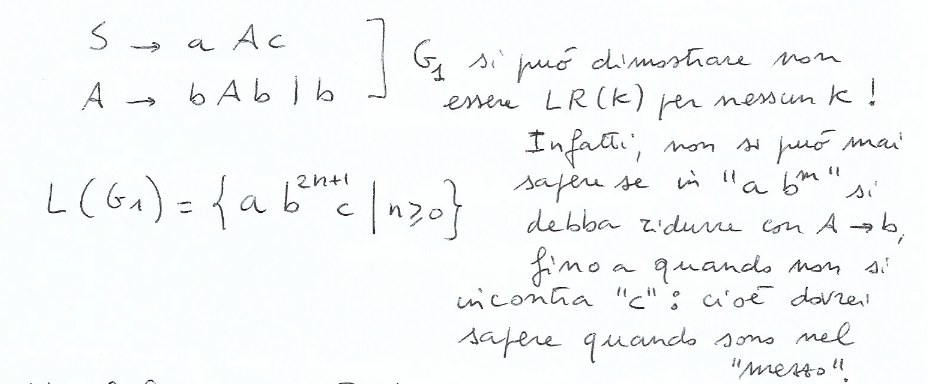
\includegraphics[width=0.7\textwidth]{img/esempio84.png}
\end{center}
Ma il linguagio generato da $G_1$ e' generabile da una grammatica LR(o)!
\begin{center}
    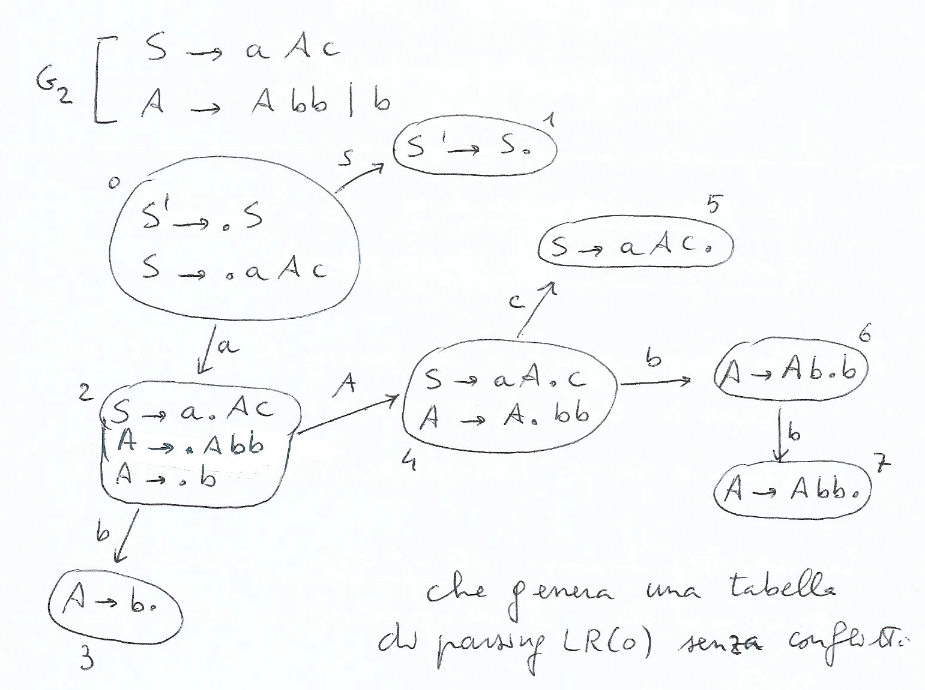
\includegraphics[width=0.7\textwidth]{img/esempio85.png}
\end{center}
\begin{center}
  $\to$ L($G_1$) = L($G_2$) e' un linguaggio LR(o)!
\end{center}
\vspace{1em}
Ricordiamo che:
\begin{itemize}
  \item Un linguaggio e' libero deterministico se e' accettato per stato finale da un DPDA
  \item Ogni linguaggio regolare e' generato da una grammatica di classe LL(1)
  \item Esistono linguaggi regolari che non sonpo LR(o)
\end{itemize}
\vspace{1em}
\textit{Teoremi}:
\begin{itemize}
  \item Un lingauaggio e' libero deterministico sse e' generato da una grammatica LR(k) per qualche $k \geq 0$
  \item Un linguaggio e' libero deterministico sse e' generato da una grammatica SLR(1)
  \item I linguaggi generati da grammatica LL(k) sono strettamente contenuti nei linguaggi generata da grammatiche SLR(1), $\forall k \geq 0$
  \begin{center}
    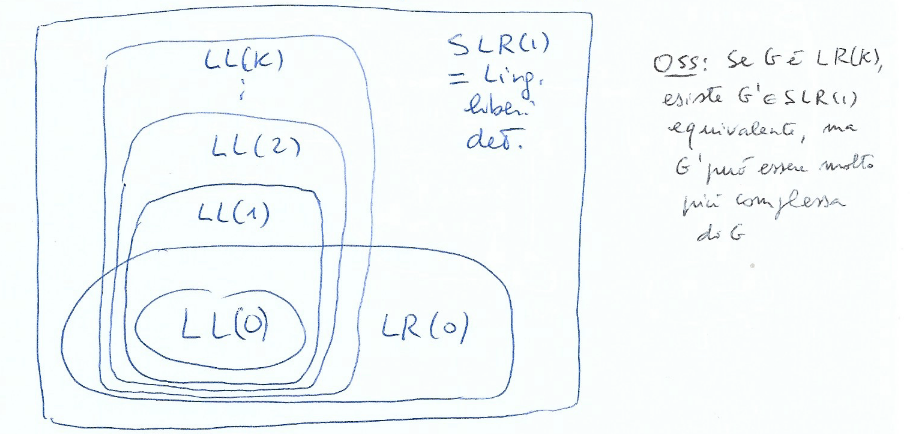
\includegraphics[width=0.7\textwidth]{img/esempio86.png}
\end{center}
\end{itemize}
\vspace{1em}
\subsection{Classificazione dei linguaggi}
Esempio
\begin{align*}
  L = \{a^i b^j \mid i \geq j \geq 0\} = a^* . \{a^n b^n \mid n \geq 0\}
\end{align*}
e' libero deterministico
\begin{center}
    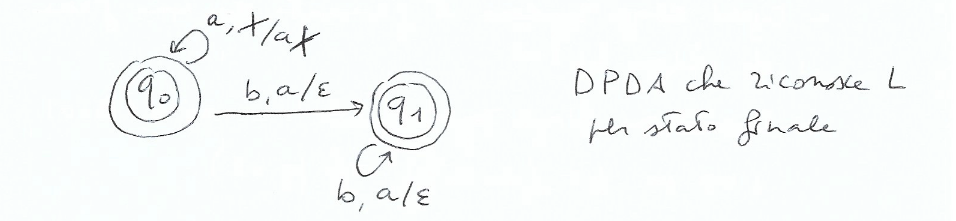
\includegraphics[width=0.7\textwidth]{img/esempio87.png}
\end{center}
\begin{itemize}
  \item L non e' LL(k) per nessun k!
  \item Tuttavia L e' SLR(1)
  \begin{center}
    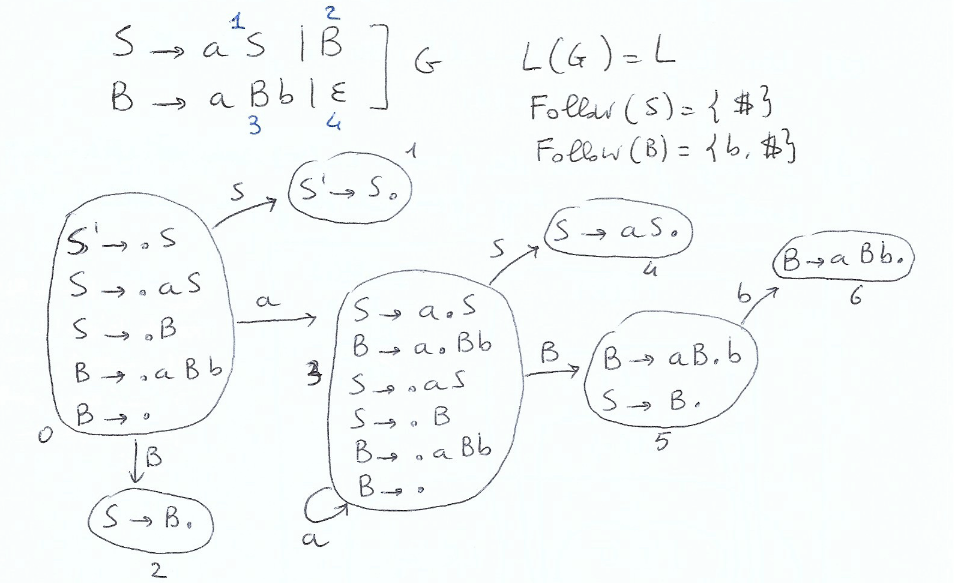
\includegraphics[width=0.7\textwidth]{img/esempio88.png}
\end{center}
\begin{center}
    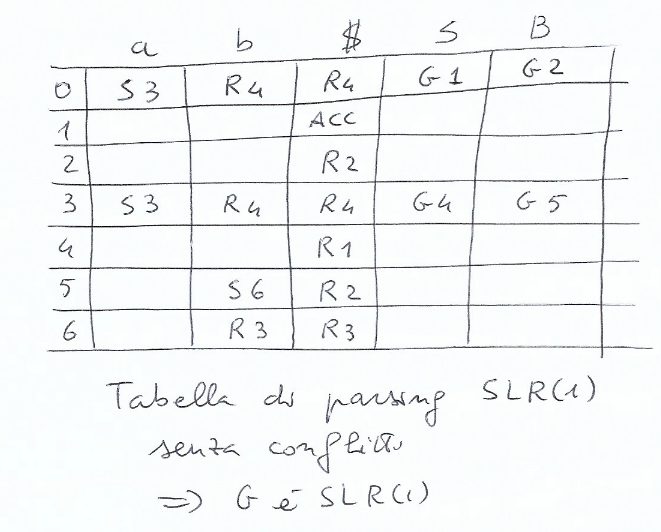
\includegraphics[width=0.7\textwidth]{img/esempio89.png}
\end{center}
\end{itemize}
\vspace{1em}
\textit{Osservazioni}: \\
1)
\begin{center}
  $L_1 = \{a^n b^n \mid n \geq 1\}$ e' LL(1) e LR(o) 
\end{center}
\begin{center}
  $L_2 = \{a^n c^n \mid n \geq 1\}$ e' LL(1) e LR(o)
\end{center}
ma $L_1 \cup L_2$ non e' LL(k) per nessun k, mentre $L_1 \cup L_2$ e' LR(o)!
\begin{center}
  $\to$ l'unione dei linguaggi LL(1) puo' non essere LL(1)!
\end{center}
2)
\begin{center}
  $L_1 = \{a\}$ e' LL(1) e LR(o)
\end{center}
\begin{center}
  $L_2 = \{ab\}$ e' LL(1) e LR(o)
\end{center}
ma $L_1 \cup L_2$ non e' LR(o) perche' non gode della prefix propriety mentre $L_1 \cup L_2$ e' LL(1)
\begin{center}
  $\to$ l'unione di linguaggi LR(o) puo' non essere LR(o)!
\end{center}
3)
\begin{center}
  $L_1 = a^* = \{a^n \mid n \geq 0\}$ e' LL(1)
\end{center}
\begin{center}
  $L_2 = \{a^n b^n \mid n \geq 0\}$ e' LL(1)
\end{center}
ma $L_1 \cdot L_2 = \{a^i b^j \mid i \geq j \geq 0\}$ non e' LL(k) per nessun k
\begin{center}
  $\to$ la concatenazione di due linguaggi LL(1) puo' non essere LL(1)
\end{center}
\vspace{2em}
\subsection{Generatori di analizzatori sintattici}
\begin{itemize}
  \item Tecniche LR (shift-reduce) sono automatizzate da molti strumenti
  \item Capostipite: YACC (yet another compiler-compiler), ma anche GNU Bison
\end{itemize}
\begin{center}
    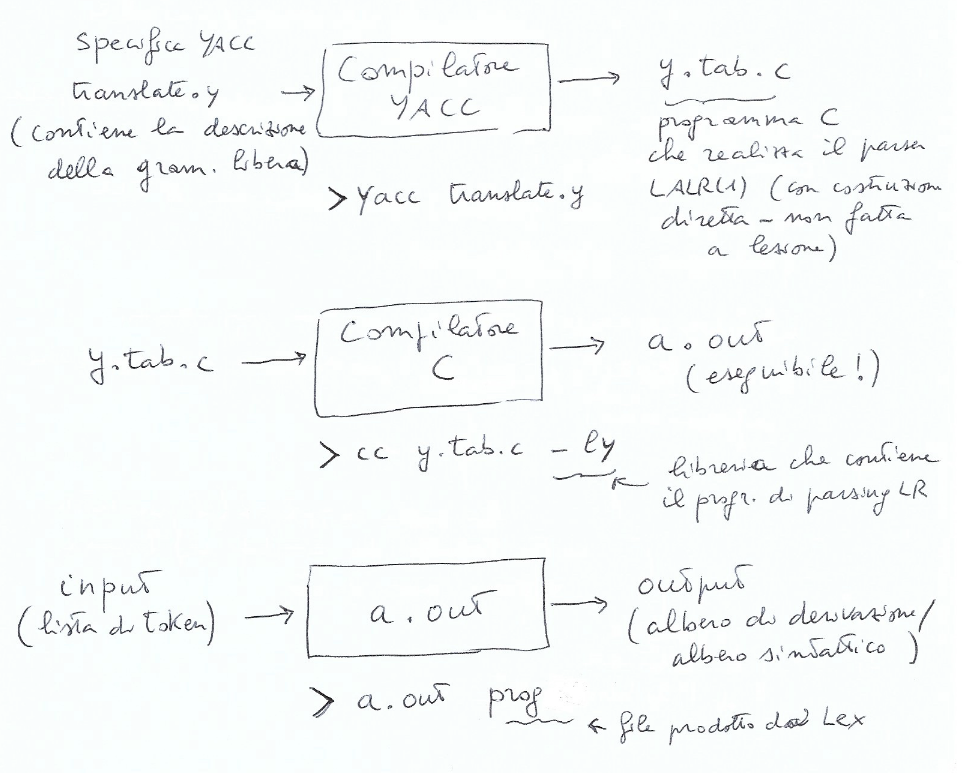
\includegraphics[width=0.7\textwidth]{img/esempio90.png}
\end{center}
\vspace{1em}
\begin{center}
  \textbf{In realta'}
\end{center}
\begin{center}
    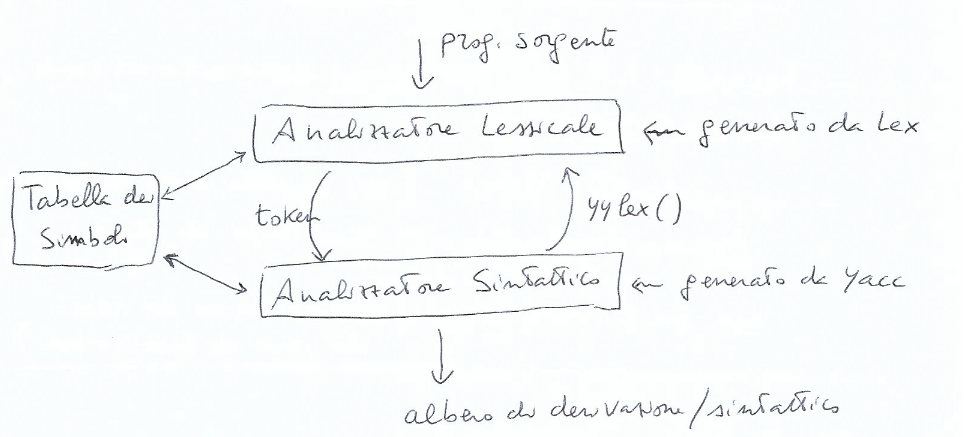
\includegraphics[width=0.7\textwidth]{img/esempio91.png}
\end{center}
\begin{itemize}
  \item L'analizzatore sintattico usa l'analizzatore lessicale come subroutine
  \item Lo invoca con \textit{yylex()} per richedere il token successivo ("on demand")
  \item alcune variabili comuni di due programmi (come ad esempio \textit{yylval}) permettono di scambiare informazioni
\end{itemize}
\subsection{Struttura di un file YACC}
\begin{center}
  $\% \{ \text{prologo} \}\%$
\end{center}
\begin{itemize}
  \item parte opzionali che contiene definizione di macro e altre dichiarazioni di variabili o funzioni che saranno usate nelle sezioni seguenti
  \item viene copiato da YACC nel suo output (\textit{y.tab.c}) in modo da procedere le definizioni della funzione "\textit{yyparse}" che effettivamente fara' l'analizzatore sintattico
\end{itemize}
\begin{center}
  definizioni
\end{center}
\begin{itemize}
  \item contiene dichiarazioni di simboli usati nella descrizione della grammatica (nomi di token, condivisi con lex) 
  \item in questa sezione e' possibile ddicharare l aprecedenza e l'associativita' di alcuni terminali/operazioni
\end{itemize}
\begin{center}
  \%\% \\
  regole \\
  \%\%
\end{center}
\begin{itemize}
  \item Una produzione della forma 
  \begin{align*}
    \text{nonterminale} \to \text{corpo}_1 \mid \dots \mid \text{corpo}_k
  \end{align*}
  e' espressa in YACC con le regole
  \begin{center}
    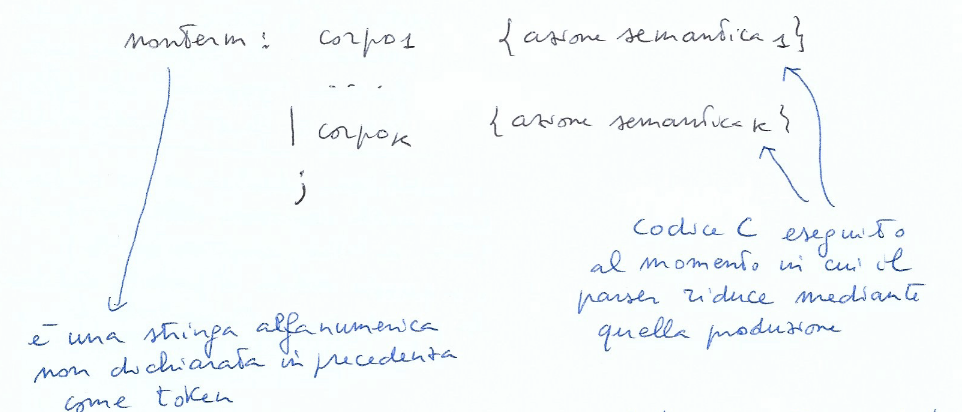
\includegraphics[width=0.9\textwidth]{img/esempio92.png}
\end{center}
\begin{itemize}
  \item un carattere tra singoli apici, '\textit{a}' e' un terminale!
  \item il simbolo inizial;e della grammatica e' il nonterminale usato nella prima regola
\end{itemize}
\end{itemize}
\begin{center}
  funzioni ausiliarie
\end{center}
\begin{itemize}
  \item contiene le funzioni di supporto per la generazione del parser;  ha queste \textit{yylex()}, funione che invoca l'analizzatore lessicale e che restituisce il nome del token (che deve essere stato definito nella sezione "definizioni" di YACC) e il suo valore (nella variabile \textit{yylval})
\end{itemize}
\vspace{1em}
\subsection{L'azione semantica}
L'azione semantica (codide C) calcola il "valore semantico" della testa della "produzione" in funzioni dei valori semantici dei simboli che compongono il corpo. \\
\vspace{5px}\\
Es: Il "valore semantico" potrebbe essere
\begin{itemize}
  \item l'albero di derivazione nel caso in cui stiamo producendo un compilatore che genera alberi esplicitamente
  \item il codice intermedio, connesso alla produzione, se andiamo direttamente a produrre codice intermedio
  \item la vera e propria valutazione dell'espressione, se stiamo in realta' producendo un interprete
\end{itemize}
In una azione semantica:
\begin{itemize}
  \item $\mathdollar \mathdollar$ si riferisce al valore semantico della testa
  \item $\mathdollar_i$ si riferisce al valore semantico dell'i-esimo simbolo nel corpo della produzione
\end{itemize}
Vediamo un esempio di file $.y$ che lavora di concetto con Lex, perche' nelle funzioni ausiliare c'e' \textit{\#include "lex.yy.c"}
\subsection{Generazione di un interprete per espressioni aritmetiche}
\begin{center}
    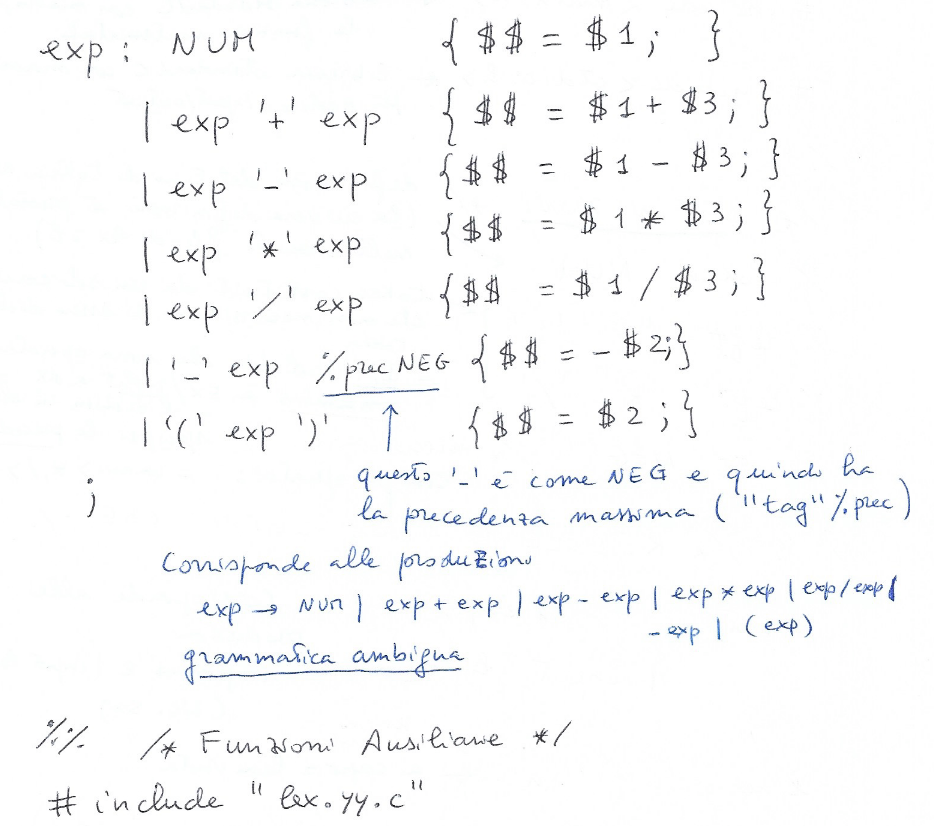
\includegraphics[width=0.9\textwidth]{img/esempio94.png}
\end{center}
$\to$ l'input e' un file con una espressione su ogni riga e il parser/interprete stampa il valore di ciascuna espressione, una per riga. \\
\textit{Nota bene}: 
\begin{itemize}
  \item Operatori dichiarati sulla stessa riga hanno uguale precedenza/priorita'
  \item Un operatore ha precedenza su tutti gli operatori delle linee precedenti
\end{itemize}
\begin{center}
    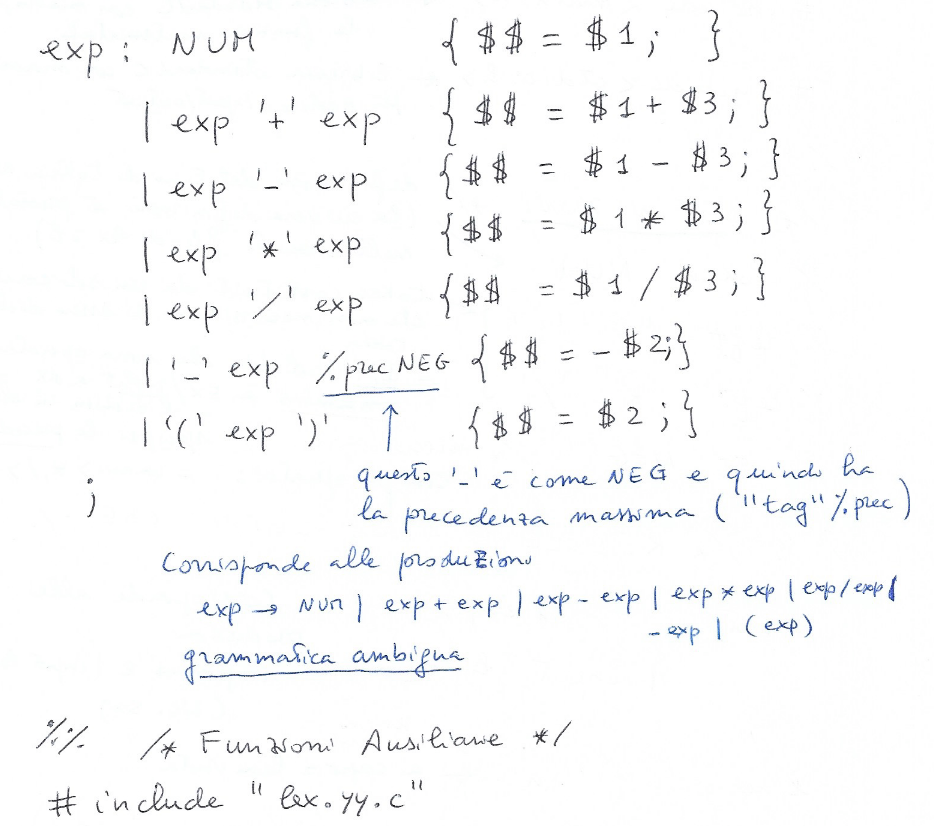
\includegraphics[width=0.7\textwidth]{img/esempio94.png}
\end{center}
La tabella LALR(1) che YACC genera, poiche la grammatica e' di base ambigua, potrebbe generare conflitti. Ma usando le informazioni aggiuntive su \textit{associativita', precedenza degli operatori} e' possibile risolvere tutti i conflitti! \\
\vspace{1em}\\
In generale YACC, in assenza di indicazioni, risolve
\begin{itemize}
  \item conflitti di tipo shift/reduce a favore dello shift
  \item conflitti di tipo reduce/reduce a favore della produzione elencata prima
\end{itemize}
E' possibile invocare YACC con l'opzione \textit{-v}. Questa opzione genera un file aggiuntivo \textit{y.output} che contiene i Kernel degli insiemi di item trovti per la grammatica, una descrizione dei conflitti generati dall'algoritmo LALR, ed anche una rappresentazione leggibile della tabella di parsing che mostra come i conflitti sono stati risolti. \\
\vspace{2em}
\section{Fondamenti: cenni su calcolabilita'}
\begin{itemize}
  \item Semantica statistica: 
  \begin{itemize}
    \item permette di fare controlli eseguiti sul testo del programma, senza mandarlo in esecuzione
  \end{itemize}
  \item Semantica dinamica:
  \begin{itemize}
    \item permette di analizzare eventuali errori a run-time
  \end{itemize}
\end{itemize}
\textit{Domanda}: possiamo rilevare tutti i possibili errori (statici o dinamici) mediante un analizzatore "statico" (cioe' senza eseguire il programma)? \\
\textbf{Ovvero}: puo' esistere un compilatore che staticamente rileva tutti i possibili errori che si verificheranno a run-time? \\
\vspace{5px}\\
Ma anche volendo essere piu' generosi, puo' esistere un programma che, anche eventualmente eseguendo parzialmente il programma oggetto, rileva in \textit{tempo finito} tutti i possibili errori a run-time? \\
\vspace{5px}\\
\begin{align*}
  check(P) = \begin{cases}
    1 \quad \text{se P e' corretto} \\
    0 \quad \text{se P presenta errori}
  \end{cases}
\end{align*}
Esiste un programma che calcola $check$? \\
Vediamo un caso specifico in cui l'errore e' la non-terminazione: se il programma e' scritto in un linguaggi sequenziale ci si aspetta che il suo calcolo termini sempre. \\
\vspace{5px} \\
Dato un linguaggio di programmazione $L$, proviamo a scrivere in $L$ un program,ma $H$ che calcola la seguente funzione
\begin{align*}
  H(P,x) = \begin{cases}
    1 \quad \text{se } P(x) \downarrow \text{"termina"} \\
    0 \quad \text{se } P(x) \uparrow \text{"diverge"}
  \end{cases}
\end{align*}
\textit{Osservazione}: Per rispondere "$0$", il programma $H$ deve riconoscere in tempo finito che il programma $P$ con input $x$ non terminera' mai il calcolo! \\
\vspace{5px} \\
Ma puo' esistere un programma $H$ siffatto? \\
Questo problema e' noto in informatica come "\textit{problema della fermata}"
\begin{center}
  HALTING PROBLEM
\end{center}
\begin{itemize}
  \item Supponiamo per assurdo che $H$ esista davvero
  \item Allora usando $H$ possiamo realizzare l'Applicazione
  \begin{align*}
    K(P) = \begin{cases}
      1 \quad \text{se } P(P) \downarrow \\
      0 \quad \text{se } P(P) \uparrow
    \end{cases} \\
    = H(P, P)
  \end{align*}
\end{itemize}
\textit{Osservazione}: Se $H$ esiste allora esiste anche $K$! 
\begin{itemize}
  \item Se $K$ esiste allora possiamo scrivere un programma $G$ che prende in input un programma $P$ e calcola
  \begin{align*}
    G(P) = \begin{cases}
      1 \quad \text{se } K(P)=0 \\
      \uparrow \quad \text{se } K(P)=1
    \end{cases}
  \end{align*}
  \textit{Osservazione}: Se $K$ esiste allora anche $G$ e' facilmente programmabile! \\
  \item Ma cosa succede se a $G$ diamo in input $G$?
  \begin{align*}
    G(G)=1 \quad \text{sse } K(G)=0 \quad \text{ sse } G(G)\uparrow \\
    G(G)=\uparrow \quad \text{sse } K(G)=1 \quad \text{ sse } G(G)\downarrow
  \end{align*}
  \textbf{ASSURDO!} $\to$ $G$ non puo' esistere $\to$ $K$ non puo' esistere $\to$ $H$ non puo' esistere!
\end{itemize}
$H$ e' il primo esempio di funzione non calcolabile (o di problema non risolvibile - \textit{Turing} 1936) \\
\vspace{1em}\\
Oltre a questo esistono molto altri problemi di funzioni che non esistono. \\
\vspace{1em}\\
Possiamo risolvere questi problemi considerando un diverso linguaggi di programmazione? Se il linguaggio e' abbastanza ricco (Turing-completo) allora NO! \\
Il problema della fermata per i normali linguaggi di programmazione e' indecibile: non esiste alcuna procedura che lo risolva. \\
\vspace{1em} \\
\subsection{Procedura di decisione}
E' una procedura che
\begin{itemize}
  \item funziona per argomenti arbitrari
  \item risponde \textit{si} o \textit{no} in tempo finito
\end{itemize}
Esempio: $w \in L(G)?$ e' decidibile per grammatiche regolari.
\subsection{Procedura di semi-decisione}
E' una procedura che
\begin{itemize}
  \item funzione per argomenti arbitrari
  \item risponde \textit{si} in tempo finito
  \item non e' in grado di rispondere \textit{no} in tempo finito
\end{itemize}
Esempio: $H'(P, x) = \begin{cases}
  1 \quad \text{se } P(x) \downarrow \\
  2 \quad \text{se } P(x) \uparrow
\end{cases}$
\vspace{1em}
La maggior parte dei problemi interessanti per i linguaggi di programmazione sono indecidibili (a volte semi-indecidibili, ma poco utili in pratica). \\
\vspace{1em}\\
\subsection{Proprieta' indecidibili}
\begin{itemize}
  \item Terminazione 
  \begin{align*}
    H(P,x) = \begin{cases}
      1 \quad \text{se } P(x)\downarrow \\
      0 \quad \text{se } P(x) \uparrow
    \end{cases}
    e' pero' semidecidibile!
  \end{align*}
  \item Divergenza
  \begin{align*}
    D(P,x) = \begin{cases}
      1 \quad \text{se } P(x) \uparrow \\
      0 \quad \text{se } P(x) \downarrow
    \end{cases}
  \end{align*}
  non e' nemmeno semidecidibile!
  \item Equivalenza di programmi
  \item Calcolo di una costante (cioe' se $P$ calcola una funzione costante)
  \item generazione di errori a run-time
  \item $\vdots$
\end{itemize}
Se consideriamo linguaggi con limitato potere espressivo, allora alcune di queste proprieta' possono essere decise. \\
Ad esempio: Se $L$ non ha $while$ allora tutti i sui programmi terminano $\to$ Terminazione e' decidibile! \\
Se un linguaggio e' Tuning-completo allora le proprieta' sopra sono INDECIDIBILI! \\
\vspace{5px}\\
Ma cosa vuol dire \textit{Turing-completo}? \\
\vspace{1em}
\subsection{Macchina di Turing}
Mdt $M=(Q,A,B,\delta, q_0, q_f)$ dove
\begin{itemize}
  \item $Q$ e' un insieme finito di stati
  \item $A$ e' l'alfabeto finito dell'input (tipicamente cifre 0-9)
  \item $B$ e' l'alfabeto finito del nastro ($AcB, \quad \underbrace{\Box}_\text{casella vuota} \in B$)
  \item $q_0$ e' lo stato iniziale 
  \item $q_f$ e' lo stato finale
  \item $\delta : Q \times B \, -o \to Q \times B \times \{sx, dx\}$ tale che $\delta(q_f, b)$ e' indefinita $\forall b \in B$
\end{itemize}
\begin{center}
    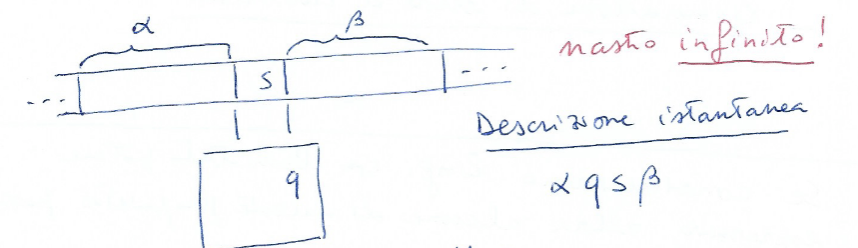
\includegraphics[width=0.7\textwidth]{img/esempio95.png}
\end{center}
Mosse:
\begin{itemize}
  \item $\zeta q s B \rotatebox{90}{$\top$} \zeta s' q' B$ se $\delta(q,s) = (q',s',dx)$
  \item $\zeta \bar{s} q s B \rotatebox{90}{$\top$} \zeta q' \bar{s} s' B$ se $\delta(q,s) = (q', q', sx)$
\end{itemize}
\begin{align*}
  L[M] = \{w \in A^* \mid q_o w \rotatebox{90}{$\top$}^* \zeta q_f B\}
\end{align*}
ma puo' non raggiungere mai ne $q_f$ ne uno stato di blocco "erroneo" cioe' puo' divergere? \\
\vspace{1em} \\
Una Mdt deterministica su alfabeto $A=[0-9]$ puo' essere vista come una macchina che calcola funzioni parziali binarie:
\begin{align*}
  f_M(w) = \begin{cases}
    1 \quad \text{se } q_0 w \rotatebox{90}{$\top$}^* \zeta q_f B \\
    0 \quad \text{se } q_0 w \rotatebox{90}{$\top$}^* \zeta q' B \not\!\rotatebox{90}{$\top$} \text{ e } q' \neq q_f \\
    \uparrow \quad \text{altrimenti}
  \end{cases}
\end{align*}
Se consideriamo l'insieme di tutte le funzioni parziali a valori binari
\begin{align*}
  \mathbb{F} = \{f \mid f : \mathbb{N} -o \to \{0,1\}\}
\end{align*}
possiamo concludere che $f \in \mathbb{F}$ e' Turing-calcolabile se $\exists \text{Mdt} M$ tale che $f_M = f$. \\
\vspace{1em} \\
\textit{Osservazione}: Ogni Mdt deterministica calcola una funziona. Allora come sara' l'insieme di tutte le funzioni Turing-calcolabili? Coincodice con $\mathbb{F}$? O esistono funzioni in $\mathbb{F}$ che non sono Turing-calcolabili? \\
La maggior parte delle funzioni in $\mathbb{F}$ non sono Turing-calcolabili!!! \\
\vspace{1em} \\
\subsection{Argomento di Cantor}
Supponiamo che le funzioni binarie (consideriamo solo le toltali, per semplicita') siano enumerabili. Dimostremo che cio' e' impossibile!
\begin{center}
    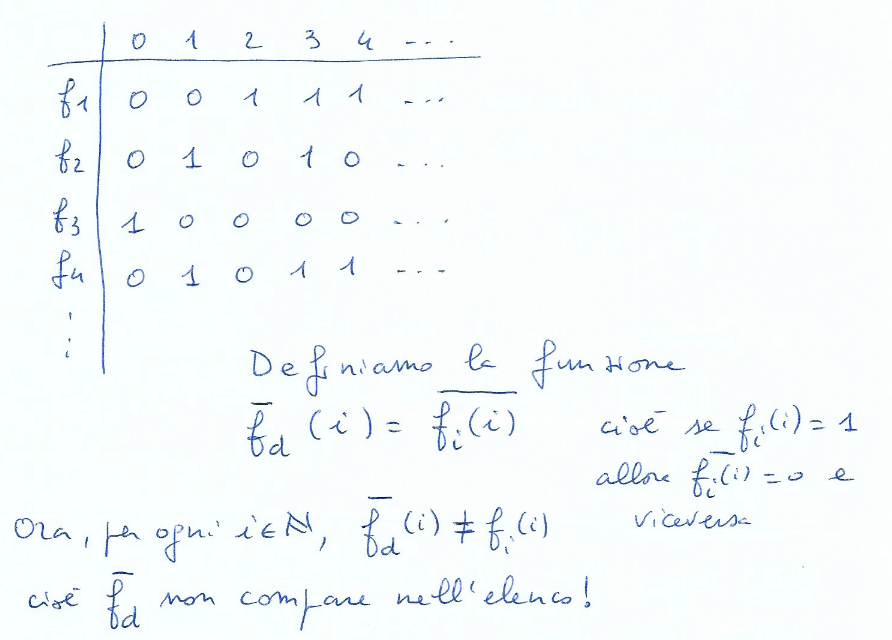
\includegraphics[width=0.7\textwidth]{img/esempio96.png}
\end{center}
In realta' si puo' dimostrare che l'insieme $\mathbb{F}$ ha cardinalita' pari ai numeri relai $\mathbb{R}$ quindi piu' grande della cardinalita' di $\mathbb{N}$. \\
\vspace{5px}\\
D'altro lato le Mdt sono enumerabili!
\begin{align*}
  M_0 \quad M_1 \quad M_2 \quad \dots
\end{align*}
$\to$ di Mdt ce ne sono tante quante $\mathbb{N}$. \\
$\Rightarrow$ La stragrande maggioranza delle funzioni non e' calcolabile! (con Mdt almeno). \\
\vspace{1em}\\
\textit{Osservazione}: Analogia con linguaggi, ovvero $P(A^*) \tripletilde \mathbb{R}$ e le grammatiche, $\tripletilde \mathbb{N}$, gia; vista ad inizio corso. \\
\vspace{1em}\\
Se cambiamo formalismo riusciamo a calcolare di piu'? 
Formalismo Turing-completo: ha la stessa potenza espressiva delle Mdt, calcola le stessa funzioni calcolabili con Mdt.\\
\vspace{5px}\\
E i linguaggi di programmazione? (C, Java, Pascal, ecc)\\
Tutti Turing-completi, purche' sia possibile usare tutta la memoria di cui possono necessitare. (Un computer ha solo una memoria finita, per cui non puo' essere equivalente a una Mdt). \\
\vspace{1em}\\
\textbf{Teorema di Jacopini-Bohm} (1996) \\
Un linguaggio di programmazione imperativo che contenga
\begin{itemize}
  \item if-then-else \quad (condizionale)
  \item while \quad (iterazione indeterminata)
  \item ; \quad (composizione sequenziale) 
\end{itemize}
(+ istruzione di assegamento) e' Turing-completo! \\
\vspace{5px}\\
\textit{Osservazione}: il linguaggio usato per spiegare la semantica \textit{sos} e' Turing-completo! \\
\textit{Osservazione}: questo teorema ha avuto un beneficio effetto nel promuovere la "programazione strutturata", cioe' quel principio di programamzione secondo il quale un linguaggio doveva contenere solo operatori ben strutturati, la cui semantica era definibile "facilmente" solo guardando i propri argomenti (non e' cosi per il Goto!) \\
\vspace{1em}\\
\subsection{Test di Church-Turing (1936-1937)}
Se una funzione puo' essere calcolata algoritmicamente in qualche formalismo, allora e' calcolabile con Mdt.
\begin{itemize}
  \item Tesi perche':
  \begin{itemize}
    \item non c'e' una definizione formali di cosa sia "algoritmicamente" calcolabile
    \item e' implicita una quantificazione universale su tutti i possibili formalismi! Infinite prove? E se domani uno arriva con un nuovo formalismo? $\dots$
  \end{itemize}
  \item Considerata vera perche' in 80 anni nessuno e' riuscito a confutarla!!
  \item Criterio di equivalenza tra linguaggi sequenzali: se $l_1$ e $l_2$ sono entrambi Turing-completo allora sono equalmente espressivi per la tesi di Church-Turing.
  \item Nel caso dei linguaggi concorrenti la questione e' diversa perche; i programmi concorrenti non calcolano solo funzioni ma risolvono problemi, offrono servizi, $\dots$.
\end{itemize} 
\vspace{1em}
\subsection{Gerarchia di macchina}
\begin{center}
  \textbf{Espressivita' vs Analizzabilita'}
\end{center}
\begin{center}
  Mdt $\iff$ grammatiche generabili $\iff$ $w \in L(M)/L(G)$? e' solo semidecidibile
\end{center}
Ma abbiamo visto formalismi piu' deboli ma significativi
\begin{center}
  PDA $\iff$ grammatiche libere $\iff$ $w \in L[N]/L(G)$? e' decidibile! \\
  Ma il problema dell'equivalenza $E(G_1, G_2) = \begin{cases}
    1 \quad \text{se } L(G_1)=L(G_2) \\
    0 \quad \text{altrimenti}
  \end{cases}$ e' indecibile!
\end{center}
\begin{center}
  DFA $\iff$ gramamtiche regolari $\iff$ $\exists(G_1, G_2)$ e' decidibile!
\end{center}
\vspace{1em}
\textit{Osservazione}: 
\begin{itemize}
  \item circuiti logici sono DFA
  \item vending machine sono DFA
  \item funzioni find / replace in text-editor sono DFA
\end{itemize}
$\to$ esistono molte "funzioni" interessanti che si possono calcolare in formalismi non Turing-completo! E su questi possiamo decidere molte proprieta' interessanti!
\end{document}
 